
%%%%%%%%%%%% 2 %%%%%%%%%%%%%%%%%%%%%%%%%%%%%%%%%%%%%%%%%%%%%%%%%%%%%%%%%%%%%%%%%%%%%%%%%%%
\chapter{ANITA Instrument and Payload}
%%%%%%%%%%%%%%%%%%%%%%%%%%%%%%%%%%%%%%%%%%%%%%%%%%%%%%%%%%%%%%%%%%%%%%%%%%%%%%%%%%%%%%%%%%
\section{Overview}
	The third iteration of the ANITA instrument, seen in Figure \ref{fig:ANITA3_hangtest}, is a broad-band radio frequency electromagnetic field transient detector and time domain voltage digitizer.  There have been four ANITA flights at the time of this thesis, numbered one through four.  ANITAI flew in the 2006-2007 Antarctic balloon campaign\cite{ANITA1}, ANITAII in 2007-2008\cite{ANITA2}, ANITAIII in 2014-2015 (the topic of this thesis) and most recently ANITAIV in 2016-2017.
	
\begin{figure}
\centering
	\includegraphics[width=0.8\textwidth]{figures/ANITA3_hangtest2_annotated}
	\caption{An image of the ANITAIII telescope during the test deployment in Palestine TX, Summer 2014.  Marked from top to bottom are two of the nine GPS antennas, the three vertically separated rings, the deployed solar panel array, and a deployed ALFA antenna.  The solar panels visible at the top of the payload are those used by the NASA Small Instrument Package (SIP).  Not visible are the ANITA instrument crate and other objects on the deck of the experiment (between middle and top antenna rings).}
	\label{fig:ANITA3_hangtest}
\end{figure}	
	
	\subsection{Signals and backgrounds}
	The ANITA instrument's scientific goal is to observe high energy particle interactions within the ice sheet of Antarctica.  The hadronic and electromagnetic showers produced by a collision between a high energy particle and the atmosphere produces radiation which can propagate with low attenuation to ANITA's stratospheric altitude. However, a low flux density has thus far prevented their detection, with phenomenological models putting detection prospects slightly beyond the grasp of previous payloads.  It has an additional detection strength for UHE cosmic ray (UHECR) interactions within the atmosphere above the continent.  The radiative emission of the resulting showers precipitated from UHECRs has two detection signatures, a direct signal and a signal first reflected off the ice-air boundary at the surface of the continent.  Cosmic ray signatures are expected to be primarily horizontally polarized with respect to the payload, while neutrino signatures will be primarily vertically polarized.  The ANITA instrument is optimized for detection and digitization of these signatures.
	
	There are two major background noise sources for the ANITA instrument: thermal Johnson-Nyquist radio frequency background present throughout the field of view, and human activity generating non-thermal anthropogenic electromagnetic radiation.  A simplified diagram showing the signal and background incident on the payload is found in Figure \ref{fig:AnitaInFlightObservable}.
	
\begin{figure}
\centering
	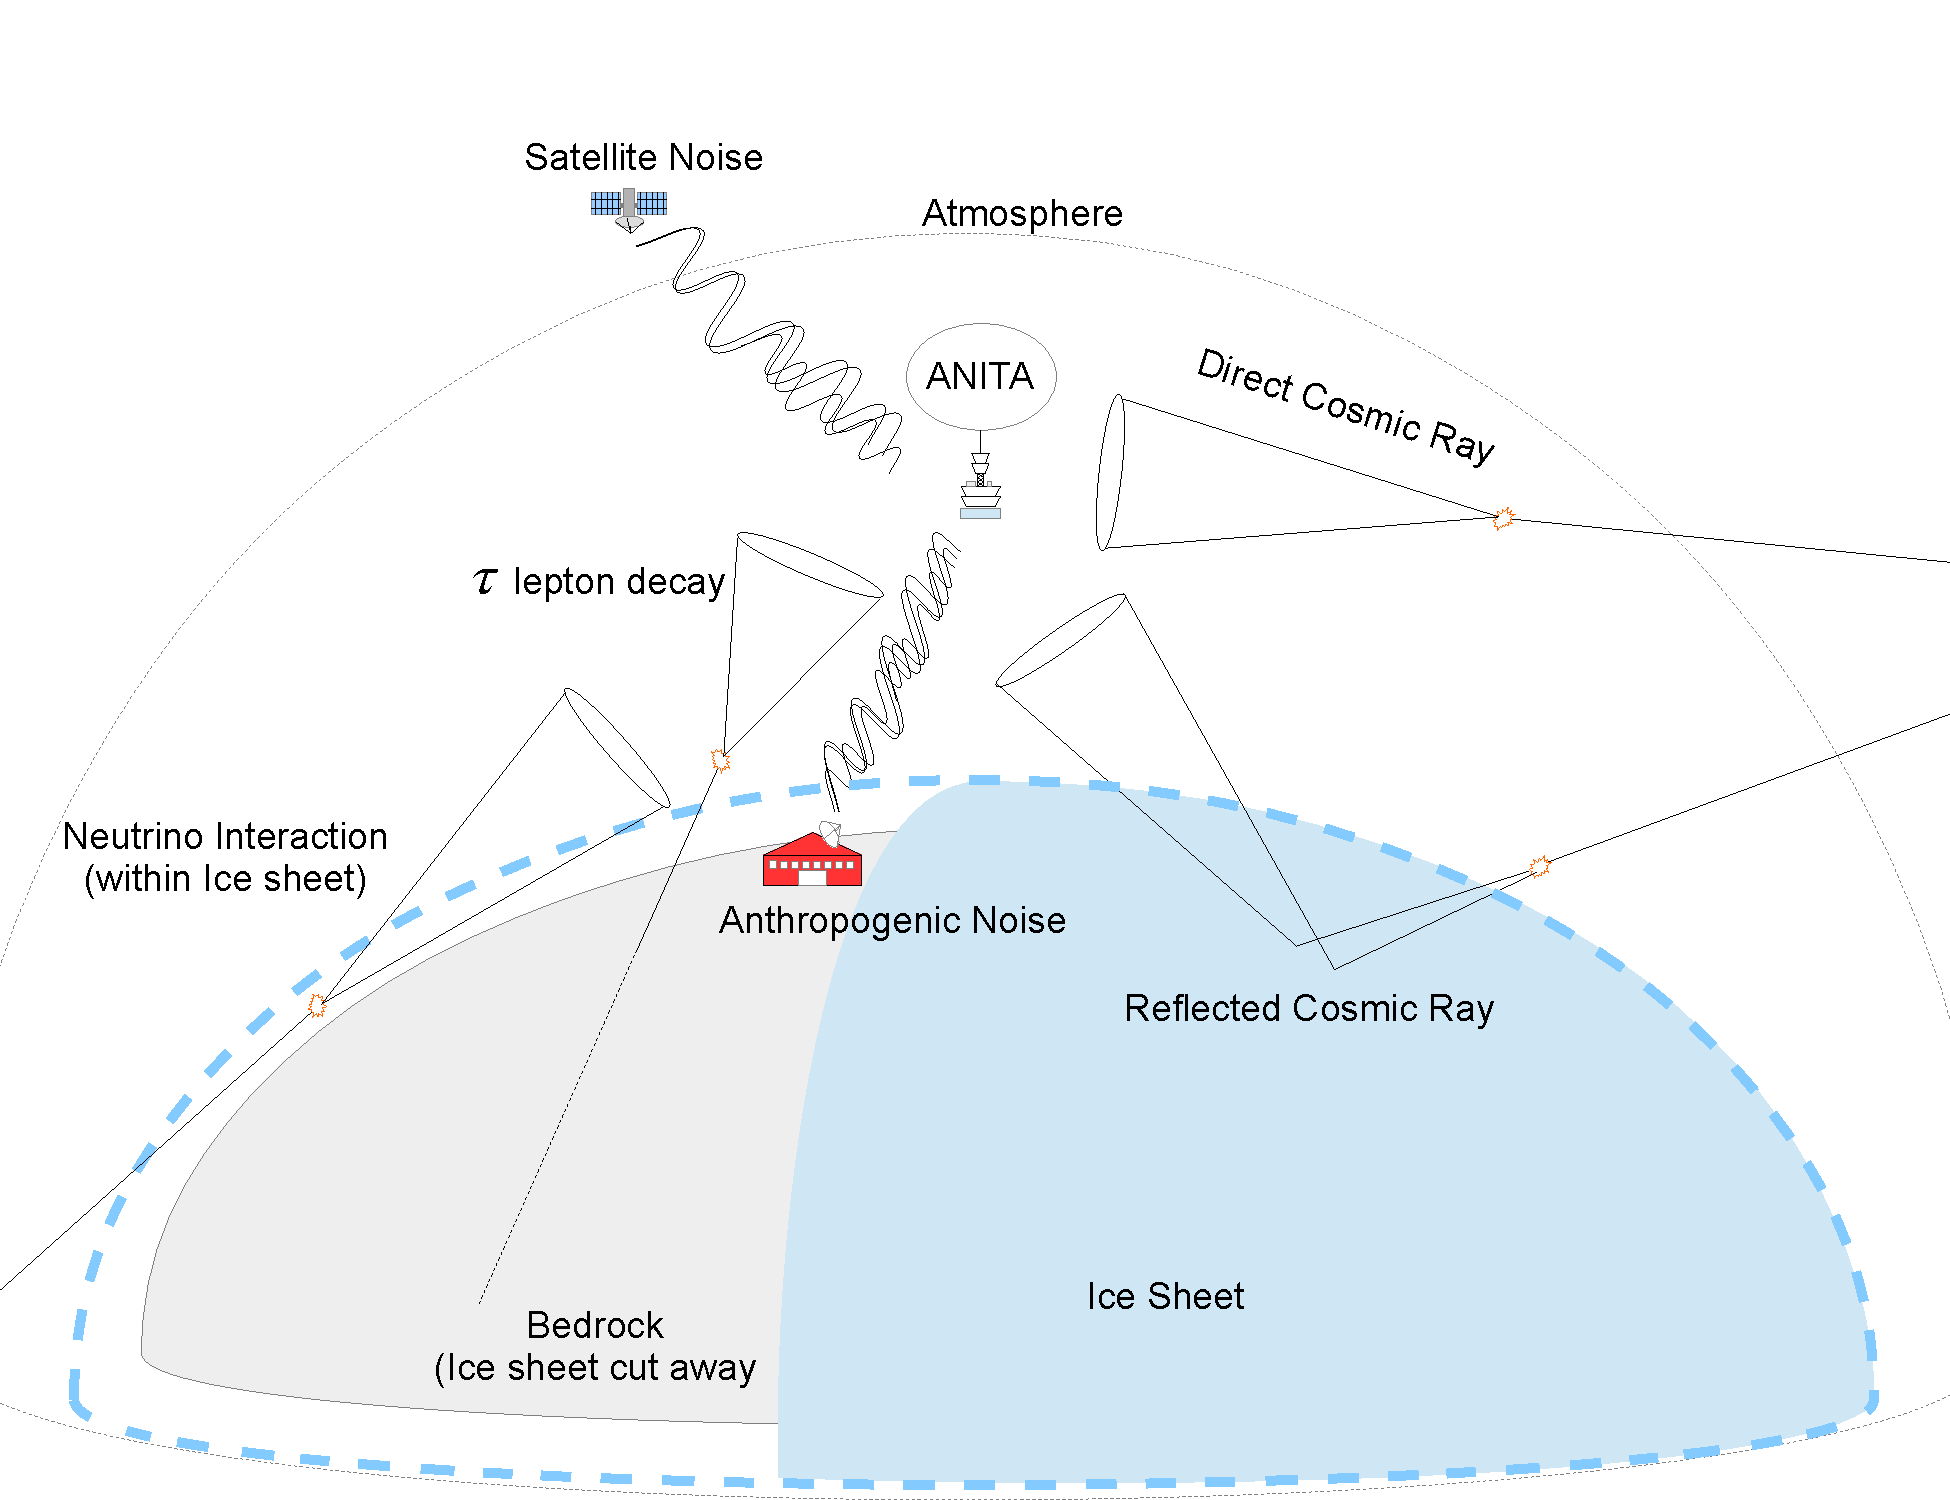
\includegraphics[width=\textwidth]{figures/AnitaInFlightObservable2}
	\caption{A cartoon of the three distinct impulsive observable signals present in the ANITAIII flight data addressed in this thesis. Not pictured is thermal background noise, which is emitted from all matter within the field of view of the instrument.  Not to scale. }
	\label{fig:AnitaInFlightObservable}
\end{figure}	

	
	\subsection{Instrumentation Overview}
	The main instrument structure consists of a collection of radially positioned, outward facing, broad-band, directional quad-ridge horn antennas.  These antennas couple the incident electromagnetic radiation into a coaxial signal line, which is then amplified through a cascaded low noise-figure amplifier chain, band-pass filtered via analog compound filters into the relevant frequency band, before finally being digitized and stored to a non-volatile hard disk. (Figure \ref{fig:RFChainBlockDiagram}).  The antennas are separated into three different vertically spaced rings, with each ring separated into 16 different azimuthally facing "phi-sectors." (Figure \ref{fig:phiSectors})  These co-pointing antennas allow multiple observations of a signal event, each with unique physical distance baseline offset between them.   The digitization is triggered by a parallel combinatoric square-law integrating power detector circuit which arrives at a decision with minimal analog waveform buffering.  After digitization, waveforms are read out via a CPCI interconnect backplane to a ruggedized, conductively cooled CPU writing to on-board redundant storage devices.  The payload is capable of reading out ~50Hz of full payload waveforms with low (\textless 5\% ) deadtime to disk.  Geographic position and relative orientation data, as well as multiple diagnostics systems, are recorded and precisely time-stamped by a GPS disciplined clock.  Selections of the waveforms and housekeeping measurements are telemetered down to ground servers for in-flight diagnostics, however full recovery of the data vaults is desired for a complete analysis.  The remainder of this chapter will expand upon these systems and the theoretical basis for their design and construction.
	
	
\begin{figure}
\centering
	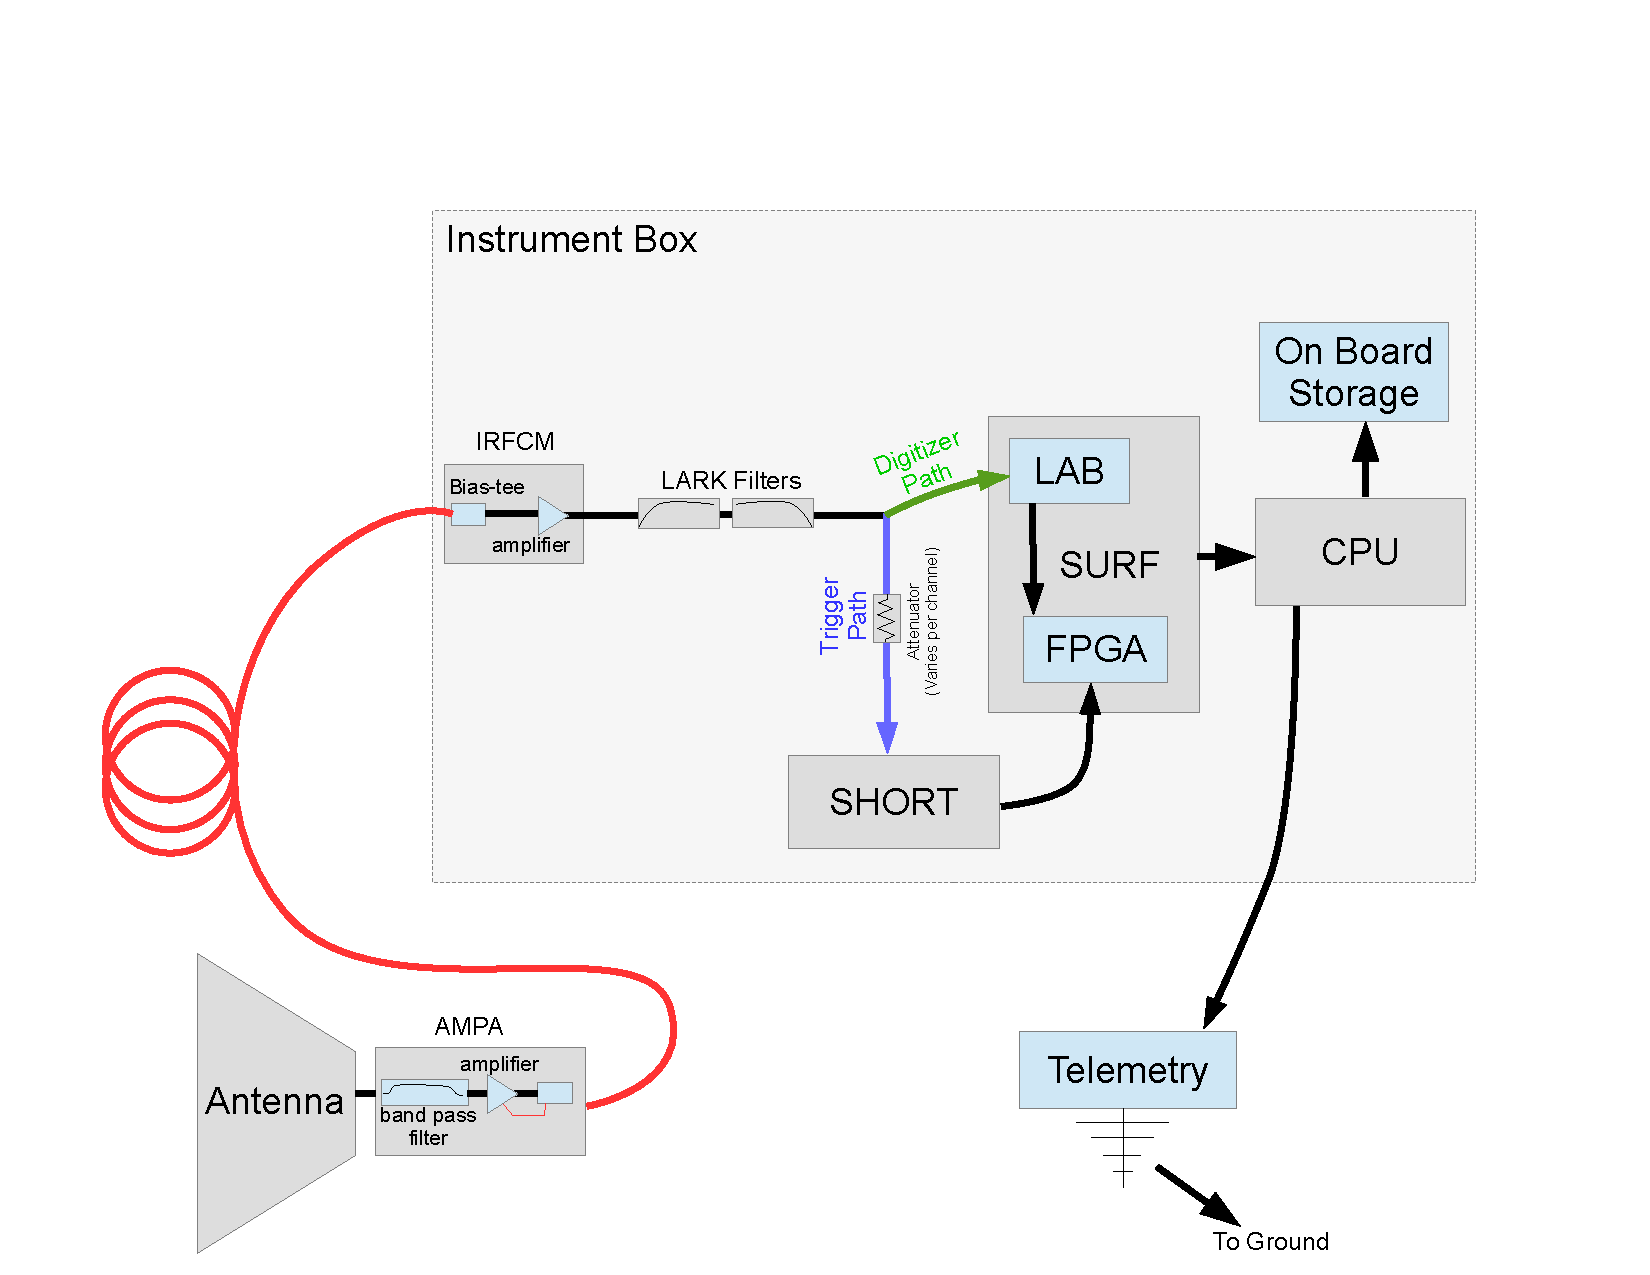
\includegraphics[width=\textwidth]{figures/RFChainBlockDiagram}
	\caption{A simplified diagram of the ANITAIII signal chain from antenna to data storage or telemetry.}
	\label{fig:RFChainBlockDiagram}
\end{figure}

\begin{figure}
\centering
	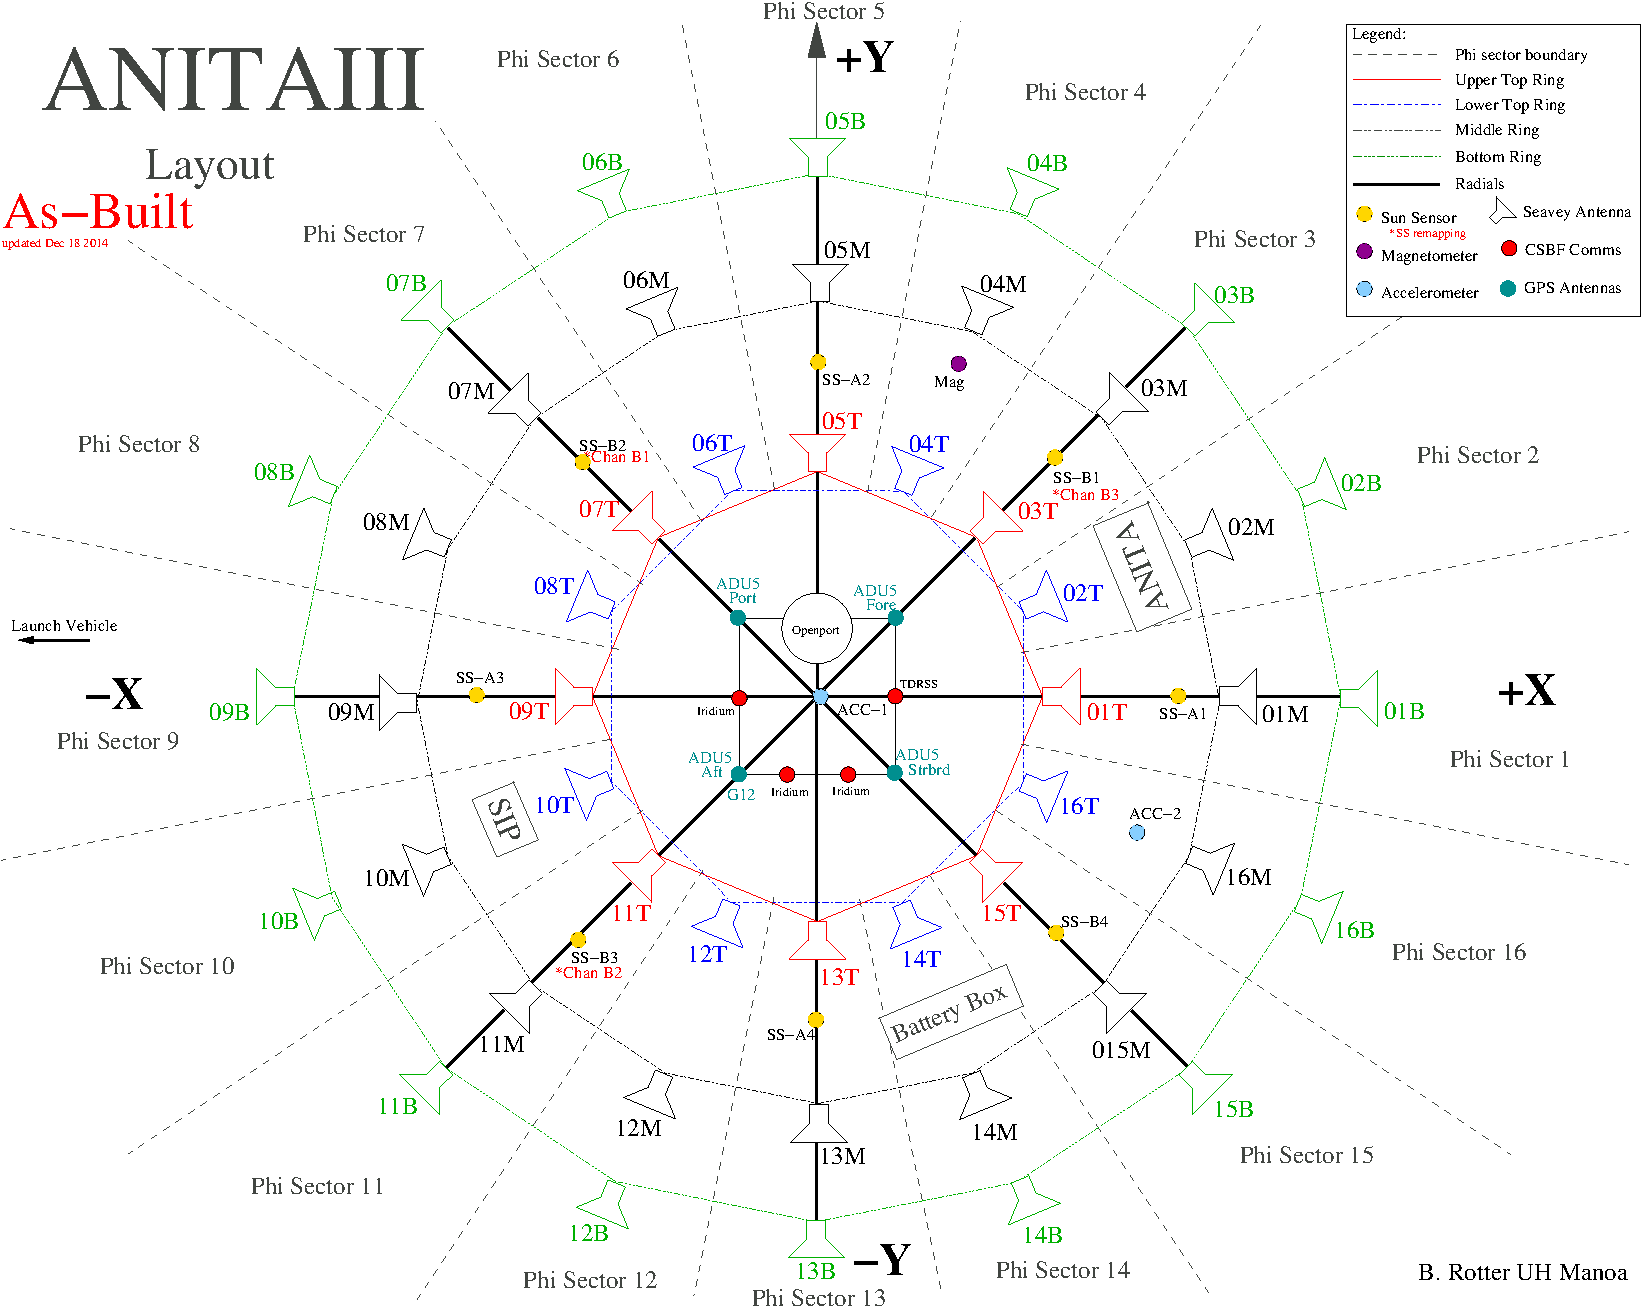
\includegraphics[width=\textwidth]{figures/ANITA3_layout_asBuilt}
	\caption{A top-down diagram detailing the locations of various components on the ANITAIII instrument as it was flown.  Visible are the locations of the NASA Support Instrument Package (SIP) and ANITA instrument box as they relate to the GPS antennas and quad-ridge antenna phi sectors.}
	\label{fig:ANITA3_asBuilt}
\end{figure}

\begin{figure}
\centering
	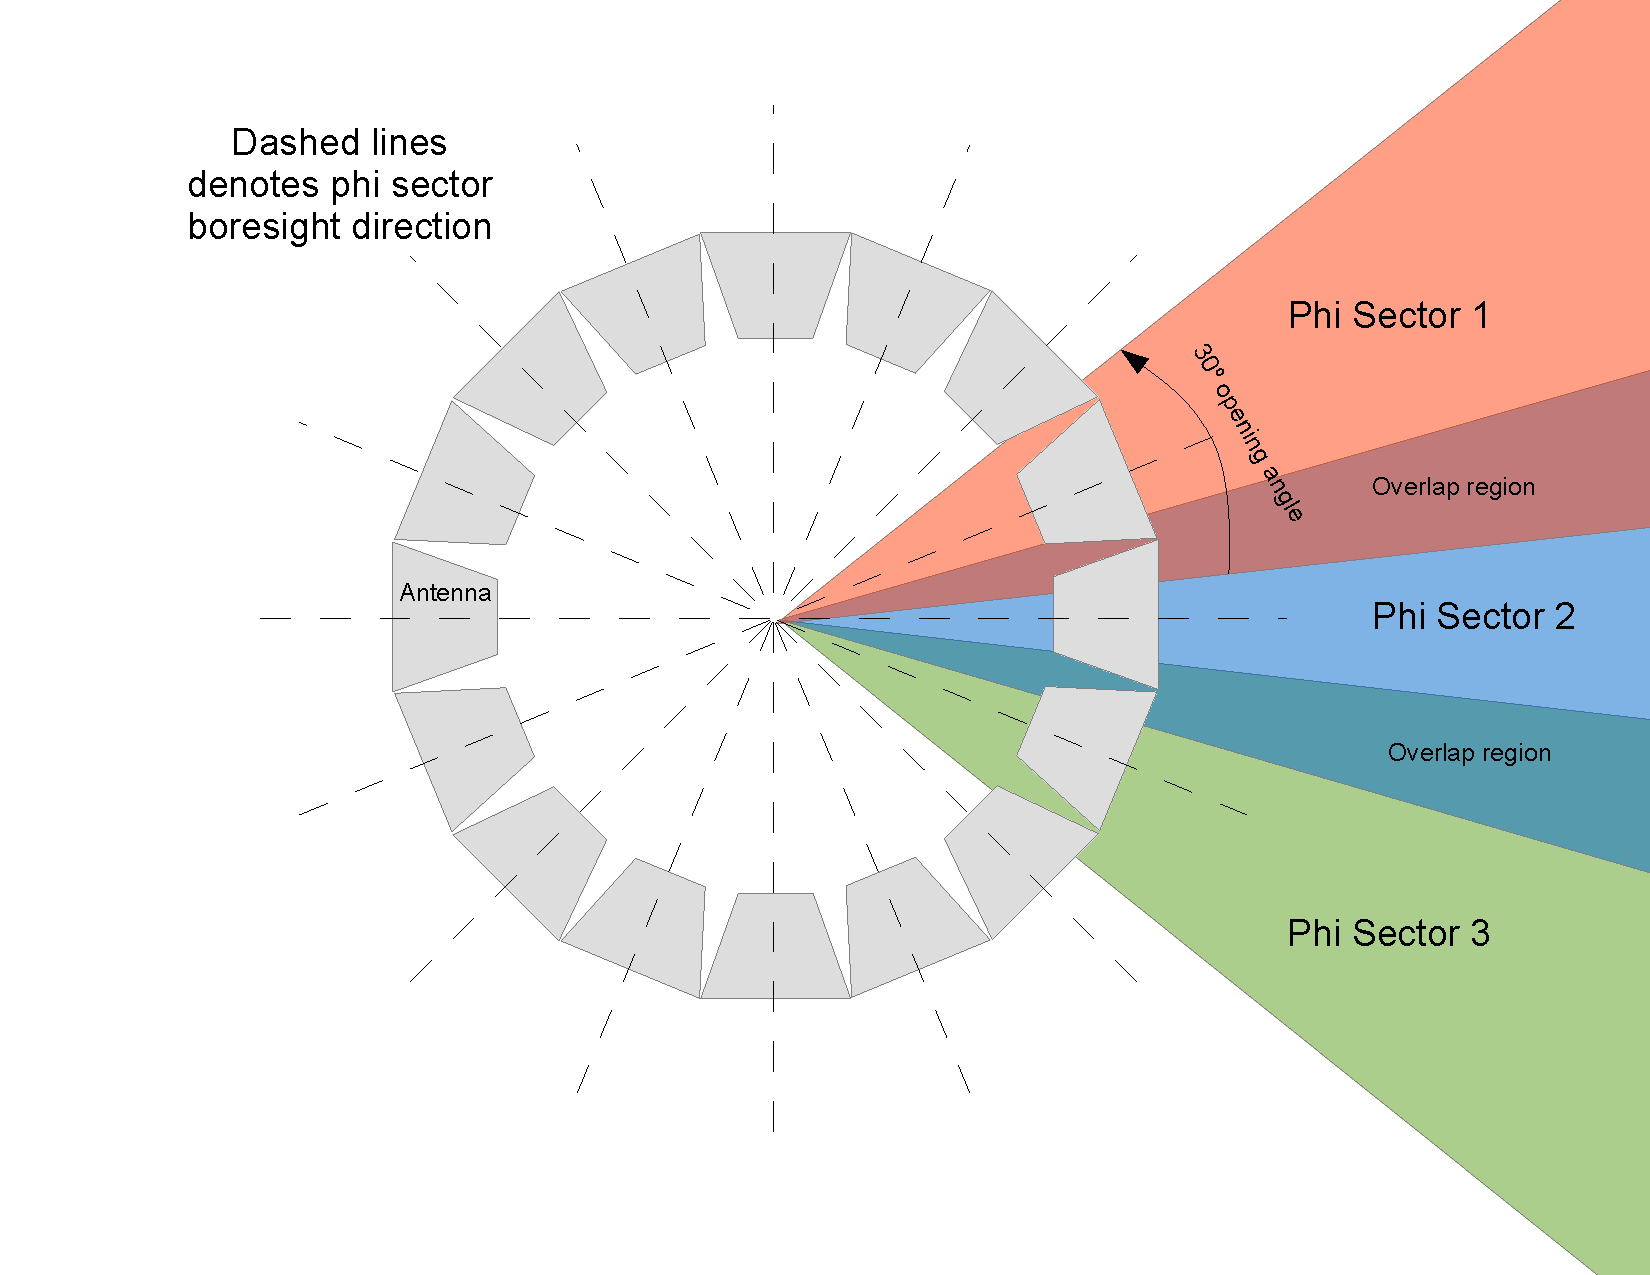
\includegraphics[width=\textwidth]{figures/phiSectors} 
	\caption{A top view of a single ring of horn antennas achieving complete azimuthal coverage.  The antennas have a  30$^{\circ}$  opening angle.  The antenna gain pattern is discussed further in the Calibration section.}
	\label{fig:phiSectors}
\end{figure}

\begin{figure}
\centering
	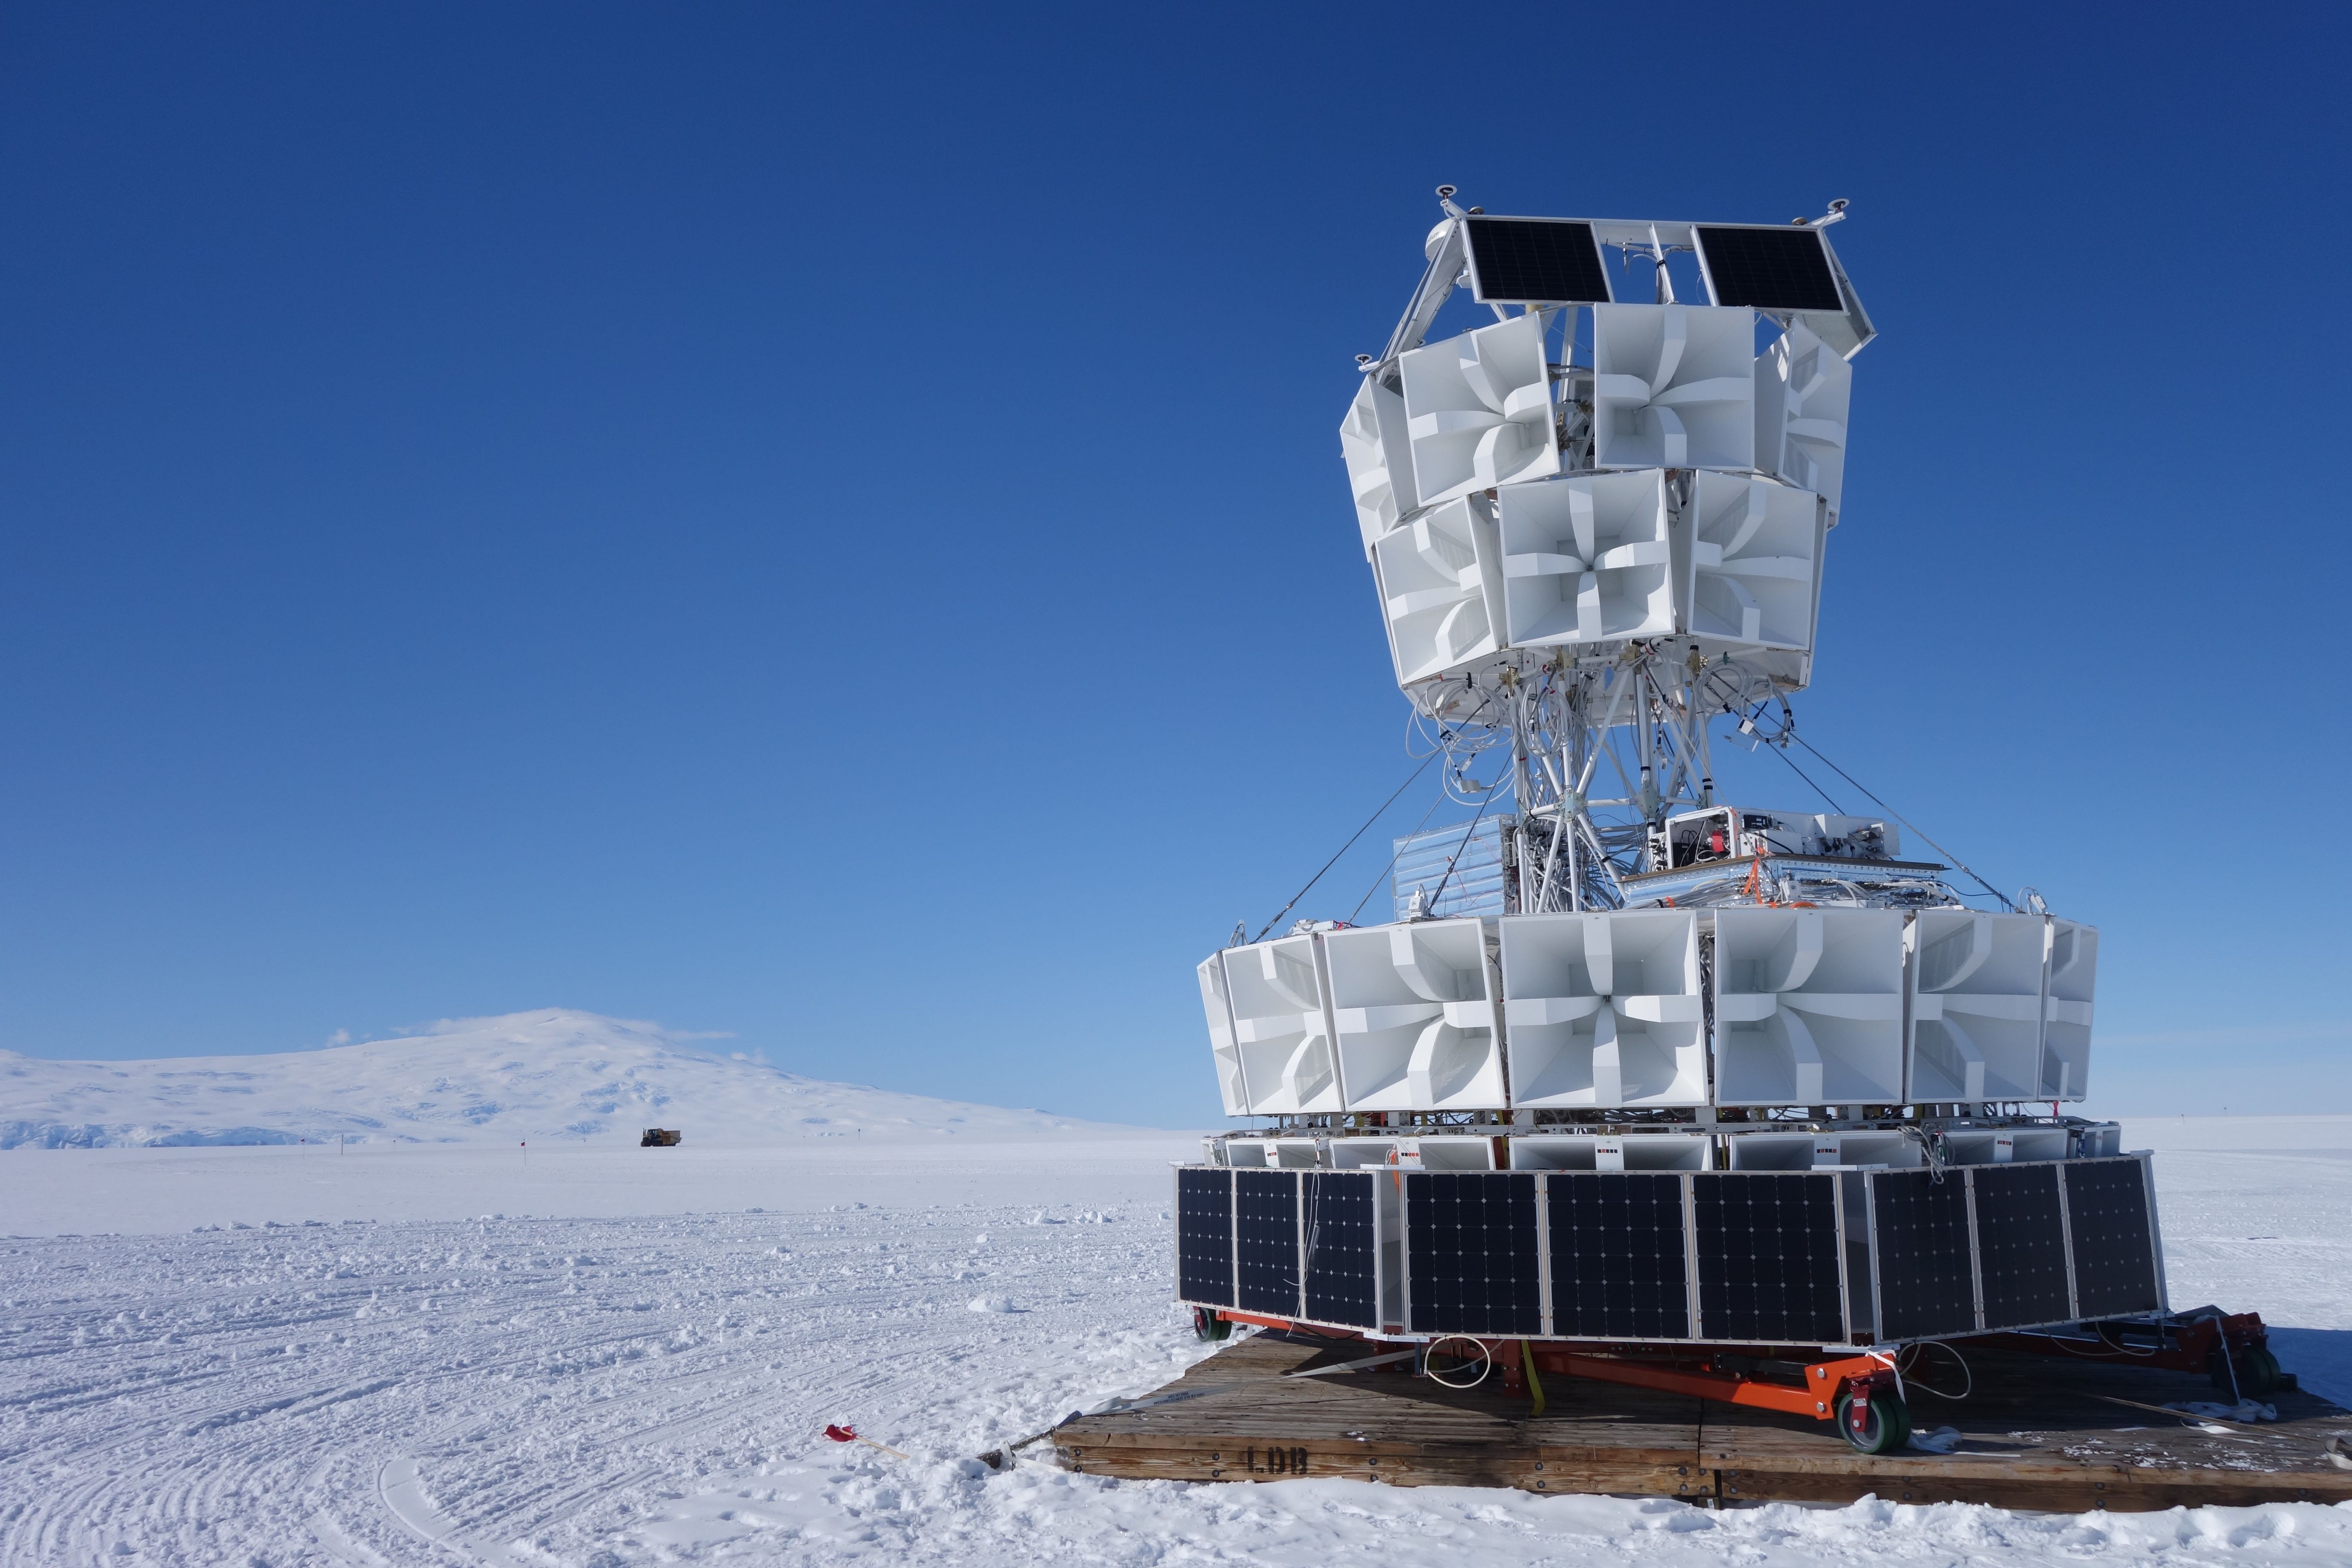
\includegraphics[width=\textwidth]{figures/ANITA3_dancefloor}
	\caption{ANITAIII during GPS calibration on the "dance-floor" at the Long Duration Balloon (LDB) facility at McMurdo Station in Antarctica, December 2014.  In the background is Mt. Erebus.  In this image the solar panels are in their retracted state, the instrument crate is visible on the left hand side of the central column, and the NASA Support Instrument Package (SIP) is visible on the right hand side. The orange structure seen under the payload is a stand used during construction and testing of the instrument.}
	\label{fig:ANITA3_dancefloor}
\end{figure}



	
\section{Antennas}
	The ANITA instrument utilizes a collection of dual polarization quad ridge horn antennas to couple the electromagnetic field incident on the payload into an electrical signal that can be digitized and stored for later analysis.  The antenna design specifications prioritize a flat gain and phase response over a gigahertz of bandwidth with a 6:1 frequency ratio, high directionality to reduce noise and boost signal fidelity, two orthogonal polarizations with roughly co-located phase centers, and light weight. 	An in-progress image of the top ring antenna assembly is shown in Figure \ref{fig:antennaAssembly} in which two sides of the antenna can be seen, and where both the RF ports and attachment mechanisms are visible.
	
\begin{figure}
\centering
	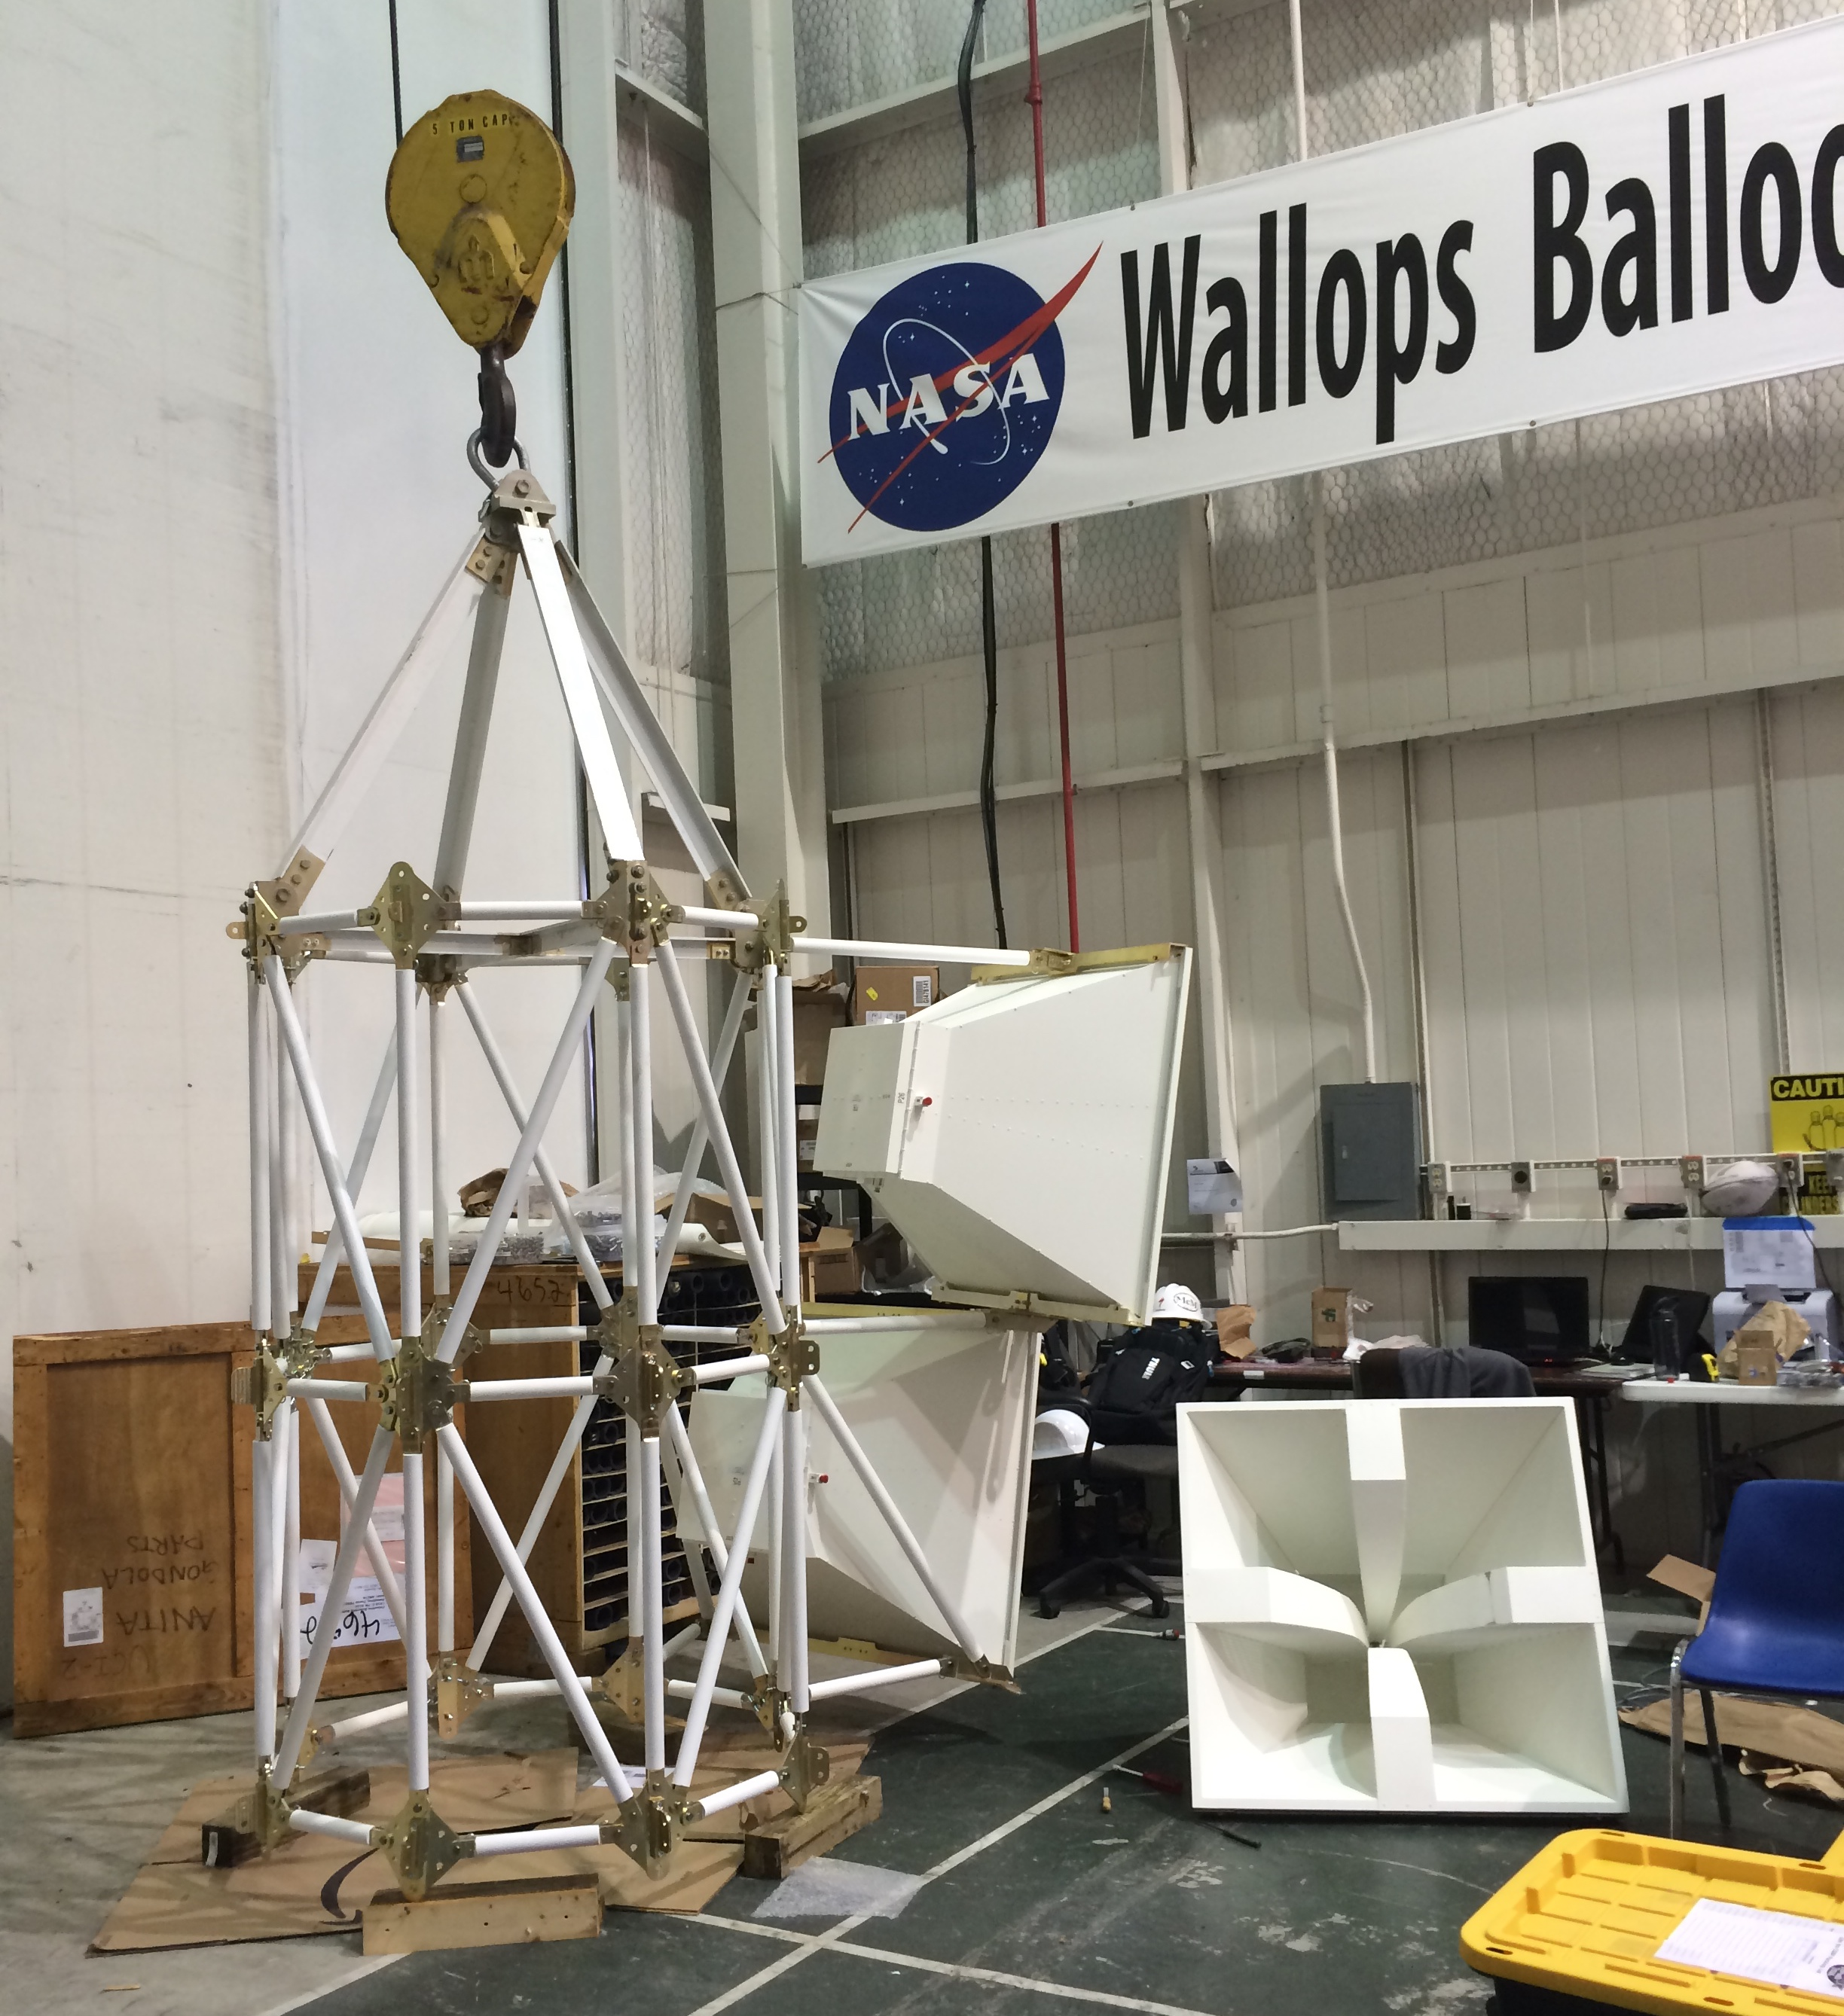
\includegraphics[width=\textwidth]{figures/AntennaAssembly}
	\caption{The top ring and apex structure of the ANITAIII payload during assembly at the Columbia Scientific Balloon Facility in 2014.  Visible is the center column of the gondola structure, three of the dual-polarization antennas, two of which have been mounted.  On the antennas the RF ports are visible, capped by red protective plastic covers.  The top ring of antennas consists of two rows of eight antennas each, which are staggered to match the two lower ring boresight directions.}
	\label{fig:antennaAssembly}
\end{figure}	
	
\subsection{Geometry and Orientation}
	ANITAI began with only two vertically separated rings and 32 antennas, however subsequent flights have packed more into the available space dictated by the flight vehicle launch envelope.  Between ANITAI and ANITAII an additional eight deployable nadir ring antennas were added that unfolded into flight position immediately after launch.  Between ANITAII and ANITAIII an additional 8 antennas were added to the lower ring, equalizing the number per phi sector and bringing the total count to 48.  ANITAIV, being a fast-turn-around re-flight, flew the same number of antennas as ANITAIII.  
	%Comparison images of these flights is visible in Figure \ref{fig:anitaGondolaComparison}
	
	Antennas are located to maximize geometric baseline distance between pairs covering the same field of view in order to maximize angular resolution recovered from interferometric pointing.  The benefits of increased baselines are discussed further in the calibration chapter.  The additional antennas added in each ANITA flight increase the number of baselines possible for this interferometric pointing. This provides a $\frac{1}{\sqrt{N}}$ incoherent noise reduction for coherently summed waveforms, increasing the signal to noise ratio of the final measured event.  
	
	The antennas are pointed at a $10^{\circ}$ downward angle to put their maximum response slightly below the horizon of the Earth, where signals are most likely to appear.  The 40km expected float altitude of the payload places the horizon at a 6 degree downward angle.  Signals of any category have their most probably observation location near the horizon, where the integrated atmospheric volume is at a maximum.
	%Maybe add an image of what the view of the antenna is
	
	The size of the antennas is dictated by the minimum desired frequency (f=C/$\lambda$), a term dominated by both physical payload launch envelope constraints as well as anthropogenic CW noise, such as FM radio transmissions, prevalent in the VHF band. Low frequency signals require large antennas, ANITAIII's 180MHz minimim frequency corresponds to a 1.6m wavelength, which, with a quarter wave excitation mode in the antenna ridges, gives a 0.42m (16.4") minimum face width.  This width matches the maximum separation of the antenna ridges, shown in Figure \ref{fig:antRidges}.  The use of a quad ridge horn type antenna, used to increase antenna directivity without adding significant dispersion, explains the additional width of the antenna geometry.
	
\begin{figure}
\centering
	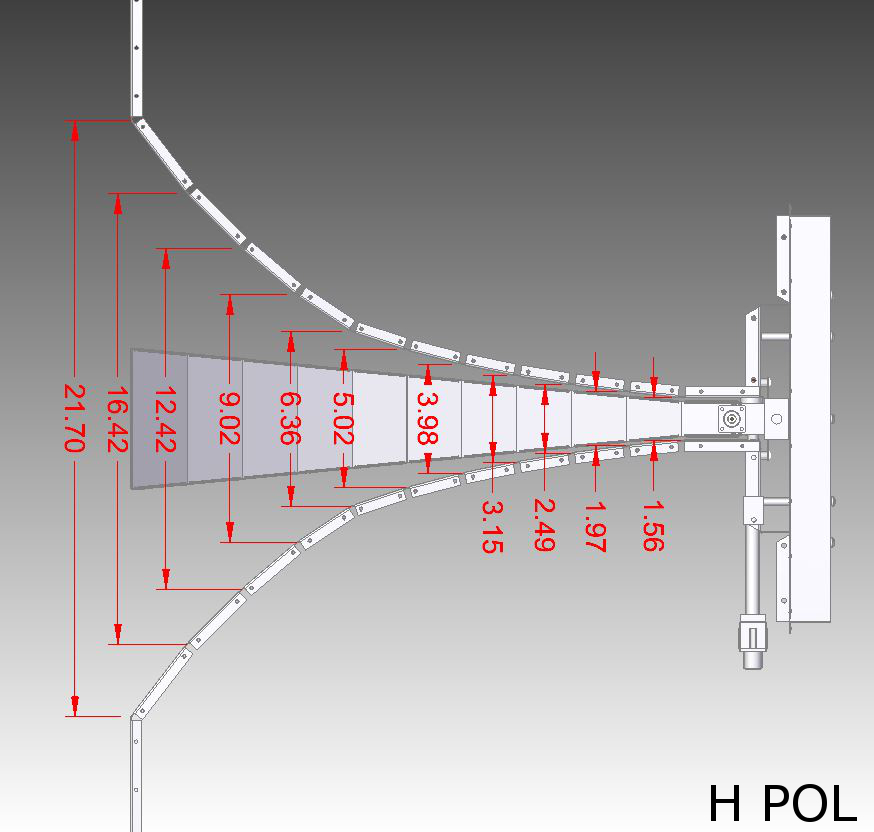
\includegraphics[height=0.45\textheight]{figures/SEAVEY_H_RIDGE}
	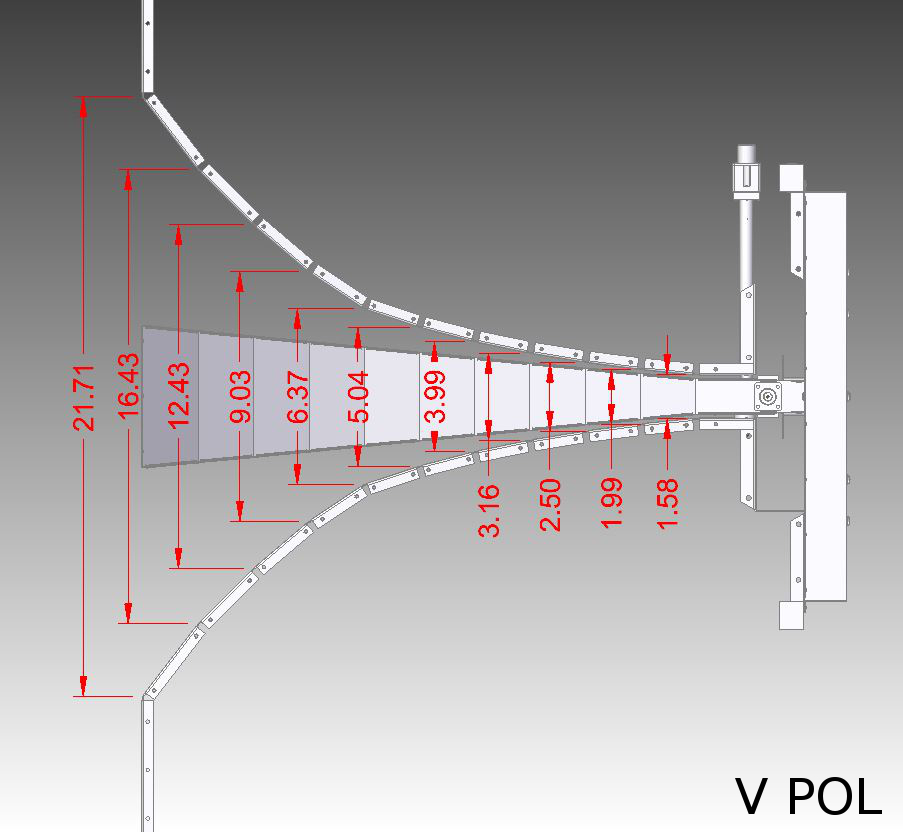
\includegraphics[height=0.45\textheight]{figures/SEAVEY_V_RIDGE}
	\caption{Measurements of the antenna ridge separation generated from the manufacturing CAD diagram by Christian Miki.  Units are in inches.  The approximately 16.4" separation corresponds to the quarter wave excitation mode for the 180MHz minimum acceptance frequency.  }
	\label{fig:antRidges}
\end{figure}	
	
	The dual, orthogonally facing polarization measurements from each antenna are desired to map out the complete Stokes parameters of any incident signal.  These two polarizations allow each antenna to contribute two signal channels covering the same solid angle to the total payload waveform readout array.  As all three possible signals will be linearly polarized at characteristic angles, a thorough understanding of event polarization is required for efficient candidate identification.  A diagram describing the primary field lines for each polarization on the antenna is shown in Figure \ref{fig:AntennaPol}.  
	
\begin{figure}
\centering
	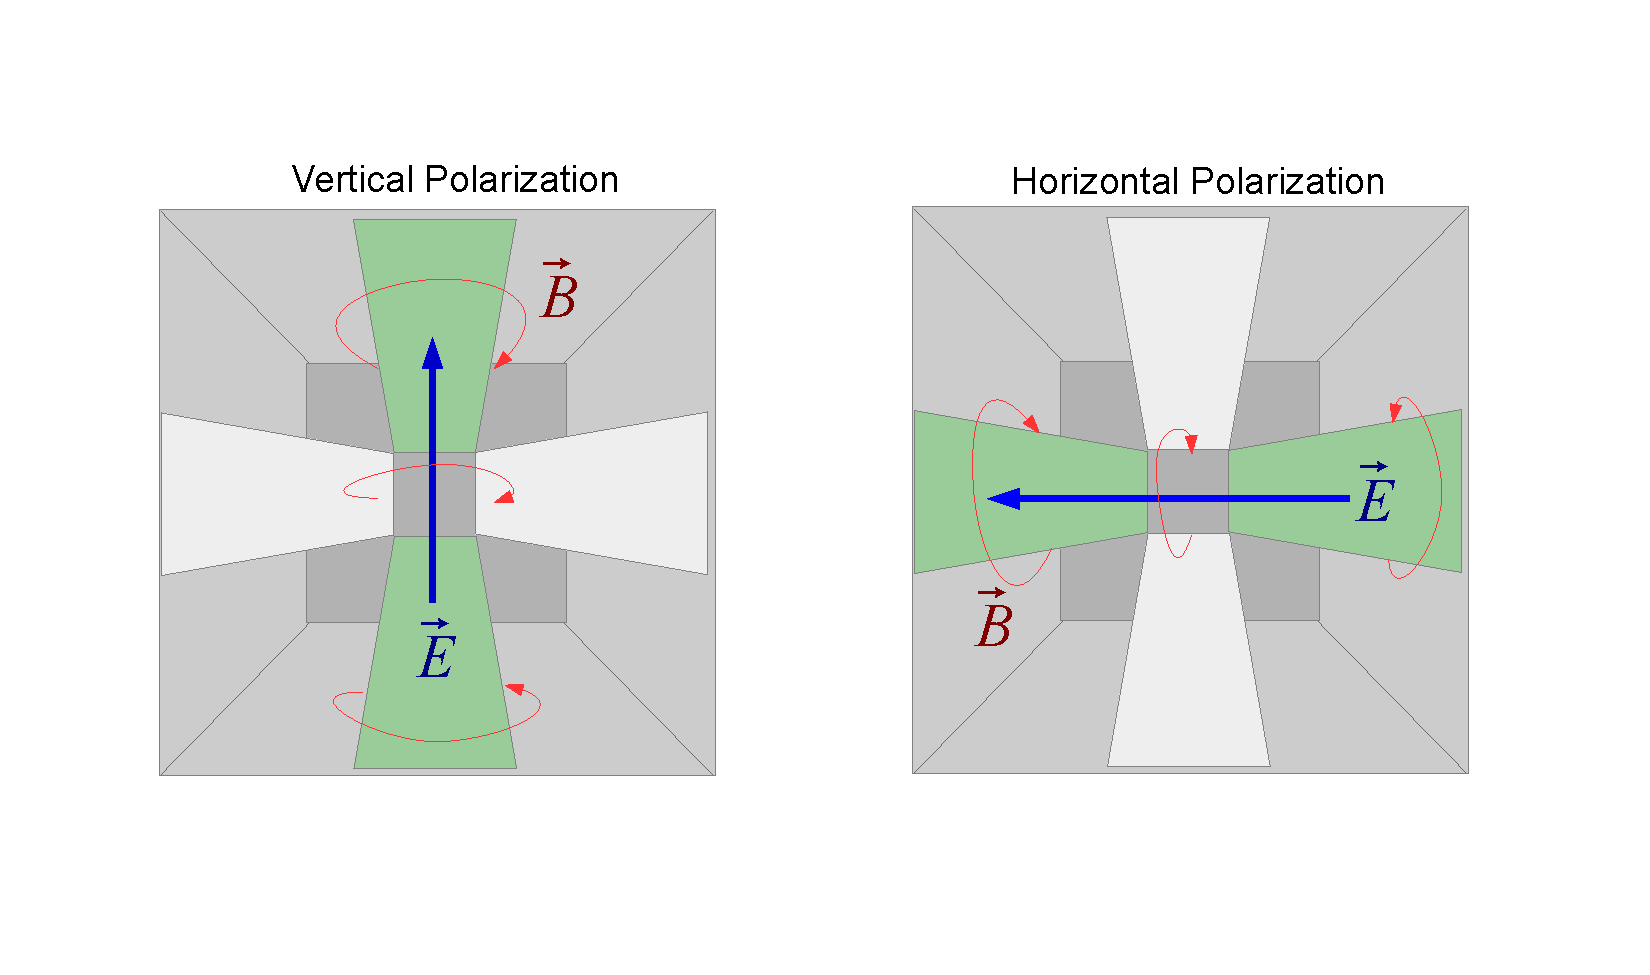
\includegraphics[width=\textwidth]{figures/AntennaPol}
	\caption{A diagram of the field line components for the Seavey dual polarization broad band horn antennas.  The E field is the principle measurement for each polarization, while the B field is the incidental cross-polarized measurement.  The antennas are specifically designed to minimize cross-polarized signal acceptance.}
	\label{fig:AntennaPol}
\end{figure}
		
	
%	Gain and directivity calibrations of the antennas was performed over a wide range of angles in multiple configurations in order to determine the full beam-pattern of the horns in both the E-field and B-field for each polarization. See Figure \ref{fig:AntennaPol} for relation between the physical antenna and measured field orientation.  These measurements were taken for the boresight of every antenna in order to determine stability of the manufacturing process.  These measurements and variations are discussed later in the Calibration chapter.
	
%	\subsection{Antenna Theory} %seems unnecessary here?  Maybe in calibration
%		An antenna is a physical object that couples the impedance of free space to that of a a coaxial transmission wire, thus effectively converting an electric field present in a medium into a voltage that can be measured.  The principle figure of interest is in this case the antenna height, which is a mathematical construct that describes the efficiency of an antenna coupling an incident electromagnetic field into a voltage on a wire.  

	\subsection{Antenna Directivity Justification}
		The ANITA instrument can utilize its geometric symmetry and full azimuthal coverage to restrict the response angle of the antennas. Increased antenna directivity improves signal response while keeping noise power constant.  ANITA is limited by thermal background noise created from the 250K surface of the Antarctic continent, the 3K CMB, and cascaded electronic amplifier noise.  Antenna thermal noise power is calculated by integrating the average temperature over the field of view of the antenna and amplifier noise is cascaded after the antenna, neither of which will vary with directivity.  However, signal power at the antenna port scales linearly with directivity. Assuming a constant efficiency, an increase in the directivity of an antenna is linearly related to its gain by Equation \ref{eqn:antGain}, where G is the antenna gain, $E_{antenna}$ is the efficiency and D is the directivity.
		
\begin{equation}
	\label{eqn:antGain}
	G = E_{antenna} * D
\end{equation}

		
		 Additionally, randomly placed and possibly unknown anthropogenic sources permeate ANITA's field of view.  Smaller antenna opening angles reduce the fractional effect that these small solid angle anthropogenic sources will have on the payload.  Maximizing antenna directivity comes at a cost of requiring additional antennas and digitization channels, increasing power consumption and complexity.
		
		There are two maximum directivity constraints that each antenna must satisfy.  First, each phi sector's response must overlap with neighboring phi sector pairs to establish azimuthal directionality from interferometric baselines. Second, their elevation must encompass both up-going reflected cosmic ray and neutrino signals, as well as have some sensitivity to earth-skimming and slight down-going air showers.  As each phi sector is $22.5^{\circ}$ separated from its nearest neighbor, a $60^{\circ}$ opening angle allows each sector to cover slightly over half the field of view of its neighbor.  For simplicity, each polarization of the antenna has symmetrical gain, which leads to a symmetric opening angle for both ridges.
		
	Measurements and calibrations of these antennas is explored further in the Calibration chapter.
	
	
	
	\subsection{ANITA Low Frequency Antenna (ALFA)}
		In addition to the quad ridge horn antennas, ANITAIII flew with an additional VHF deployable "quad-slot" antenna with an omni-directional azimuthal response (Figure \ref{fig:ALFA} mounted underneath the main structure, pictured in Figure \ref{fig:ALFA}.  The frequency response of the antenna was designed to sit below that of the main instrument, capturing waveforms from 40 to 80 MHz.  As many radio frequency EAS experimental measurements are done at lower frequencies, this antenna was added to allow direct comparison between ANITA's observed particle track radiation events and those at ground based observatories.  Due to a lack of additional digitization channels in the system, as well as on-board high-pass analog filtering on the SURF board, this antenna was heterodyned with a 900MHz Local Oscillator (LO) to up-convert the signal to a measurable frequency before being combined with channel 05TH.  05TH in turn was low-pass filtered to remove its signal and noise contribution in this signal region.  This non-symmetry in the system must be remembered in all analysis steps, and is discussed further in the calibration section.
		
\begin{figure}
\centering
	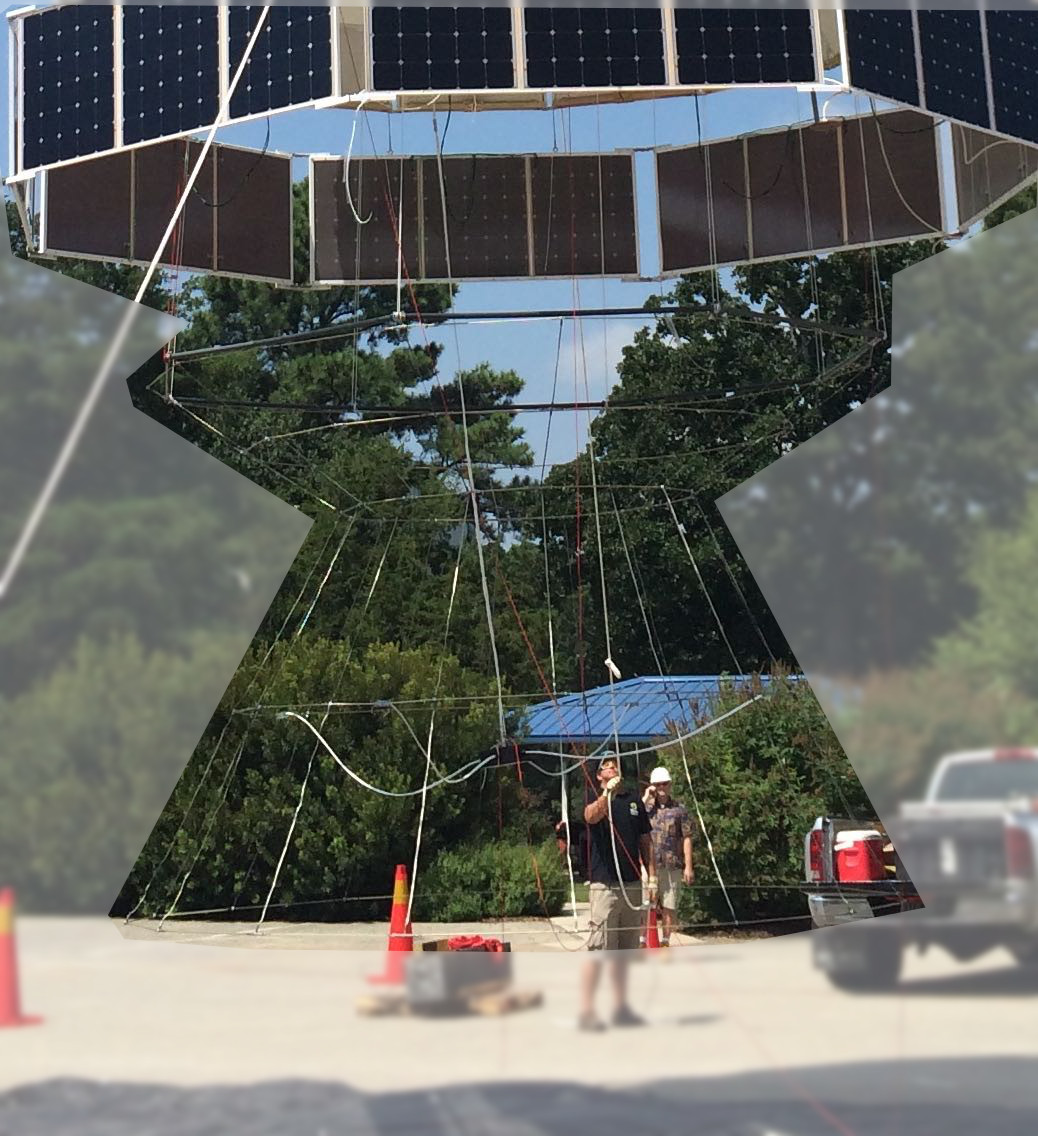
\includegraphics[width=\textwidth]{figures/ALFA_pic}
	\caption{Photo of the deployed ALFA antenna in the 2014 hang test of ANITAIII in Palestine Texas.  The photo has been modified to emphasize the outline of the antenna.}
	\label{fig:ALFA_pic}
\end{figure}


% I need a better quality image for this
\begin{figure}
\centering
	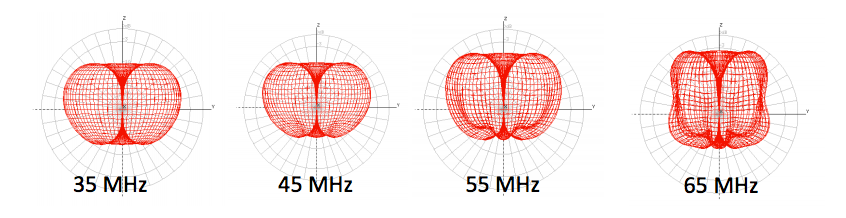
\includegraphics[width=\textwidth]{figures/ALFA_gainPattern}
%	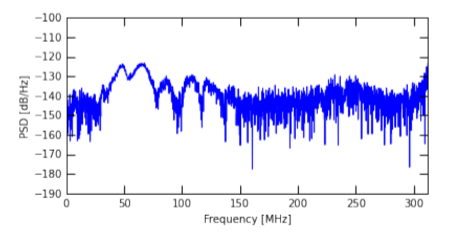
\includegraphics[]{figures/ALFA_gain}
	\caption{Top: Simulations of the expected antenna gain  pattern for the ALFA antenna.  Image provided by Andres Romero-Wolf.}
%	\caption{Top: Simulations of the expected antenna gain  pattern for the ALFA antenna.  Image provided by Andres Romero-Wolf.  Bottom: Measured in flight frequency response of the ALFA antenna.  Image provided by Stephanie Wissel}
	\label{fig:ALFA}
\end{figure}


\section{Filtering}
		The radiative power from an Askaryan or EAS geomagnetic signal both have a wide bandwidth, however there are a few considerations that require the signals read by the ANITA telescope be band limited.
		
		At the high frequency end of the spectrum, above 1.2GHz, the individual radiative particles in the shower core begin to be resolved, resulting in a loss of coherence of radiated power above that band.  This is visualized in Figure \ref{fig:CROffAngle}.  This effect is stronger at angles further from the peak Cherenkov angle away from the shower axis.\cite{PhysRevD.84.103003}  This lack of coherent signal power in the UHF region provides a high frequency suppression to the total signal bandwidth.


\begin{figure}
\centering
	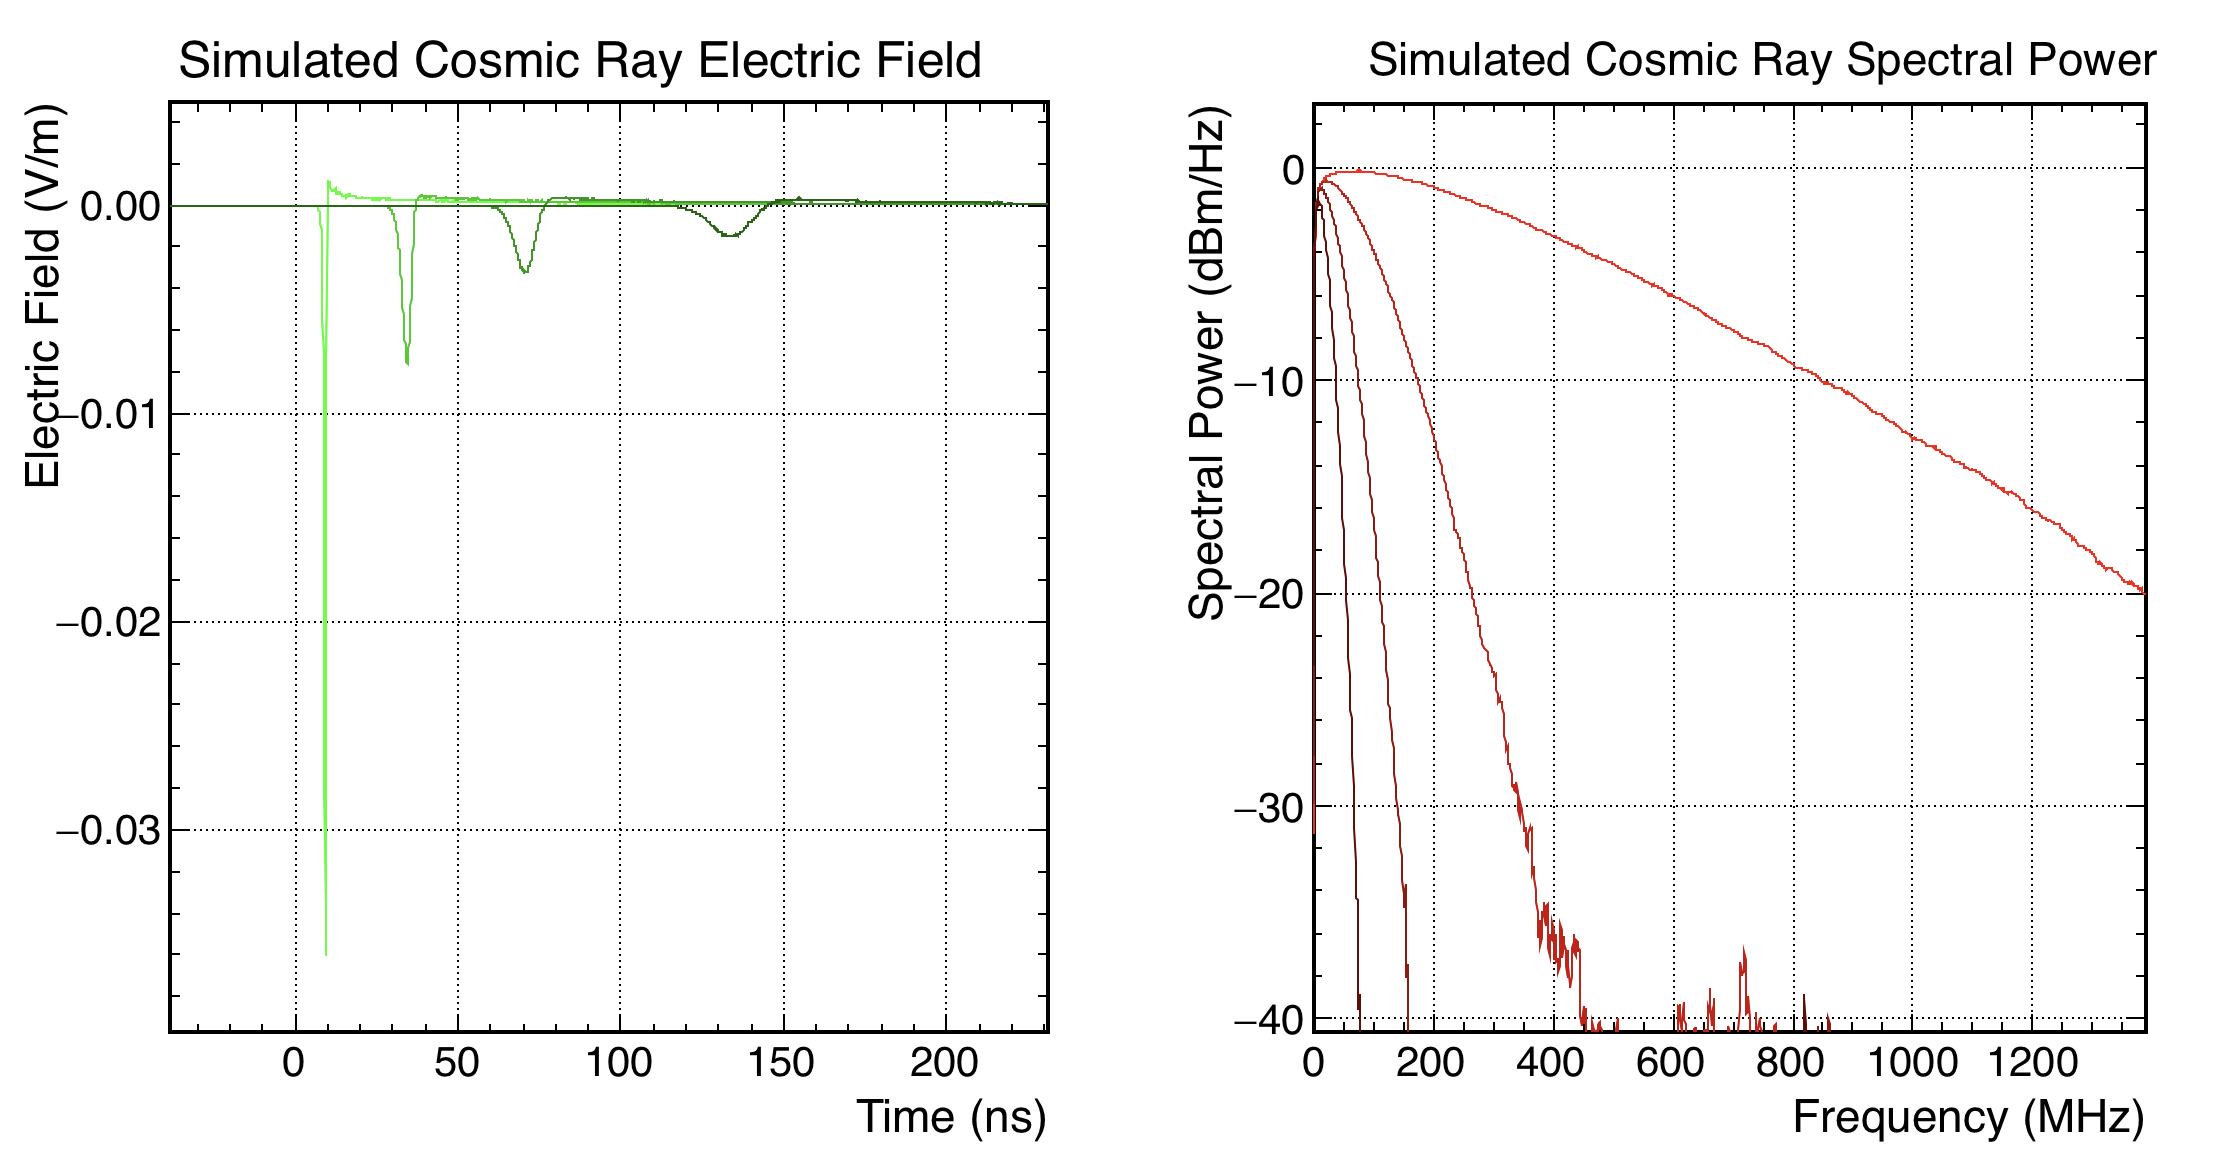
\includegraphics[width=\textwidth]{figures/CosmicRayOffAngle}
	\caption{ZHAires simulated UHECR electric field radiation transients at, and off, the critical coherence angle.  Left: The peak coherence angle of the shower radiation, with increasing distances offset from that peak in darkening hues.  The highest amplitude pulse bright green is the peak of the Cherenkov ring.  Right: The frequency power spectrums in corresponding hues of red.  As can be seen, high frequency power is significantly reduced while observed at locations away from the critical angle,  }
	\label{fig:CROffAngle}
\end{figure}	

		On the low frequency end of the spectrum, the radiated power from the shower is expected to rise as a function of frequency up to 1GHz.  Manufacturing and design limitations of a long wavelength antenna coupled with the high utilization of the VHF band by radio transmitters on satellites and ground stations lead to a requirement that lower frequencies, below 180MHz in the case of ANITAIII, be removed.
		
	\subsection{Multiple Stages}
		This band pass filtering is done in two stages, one immediately after the antenna, before the pre-amplifier in order to prevent saturation of the pre-amplifier from out of band signals, and one after the amplification chain in order to remove out of band amplifier noise.  The primary filter must have an extremely low in-band loss, as any loss introduced by the filter is observed as backfilled broad spectrum noise temperature, a value which is cascaded through the entire amplification chain.  This was accomplished with a custom made LARK band pass filter.  The secondary filtering was accomplished with two discrete low-pass/high-pass filters that do not require such a low in band loss characteristic due to their position in the signal chain.
		
	\subsection{Digitizer Bandwidth}
		The LABRADOR digitizer also influences the selection of the band edges.  The maximum sampling rate of 2.6GS/s yields a 1.3GHz Nyquist sampling frequency, however the 3dB analog bandwidth of the LABRADOR is limited to 800MHz\cite{LABASICPAPER}.  Any out of band power will be aliased into the signal band and present itself as increased in-band noise\cite{NyquistSampling}. 
		
\section{Amplification}
	The extremely low expected signal power incident on the payload must be significantly amplified in order to have a detectable amount of power.  The amplification for the ANITAIII instrument was accomplished with two stages, one close to the antenna within the custom built module, and one upon entering the instrument crate itself within the iRFCM (internal radio frequency conditioning module).  
	
	\subsection{First Stage Amplifier: The AMPA and DDAMPA}
		The front end amplification was accomplished by two similar custom built modules named the Antenna Mounted Pre-Amplifier (AMPA) and the (historically named) Drop Down AMPA (DDAMPA).  The internals for the AMPAs and DDAMPAs are diagrammed in Figure \ref{fig:AmpaDDampaBlock} and images of the modules are shown in \ref{fig:AMPAandDDAMPA}. Each enclosure contains components for filtering, amplification, and a bias network power trasmission component.  A summary of the gain and noise figure measurements for the ensemble of units is shown in Figure \ref{fig:AMPAandDDAMPA_std}.
		
\begin{figure}
\centering
	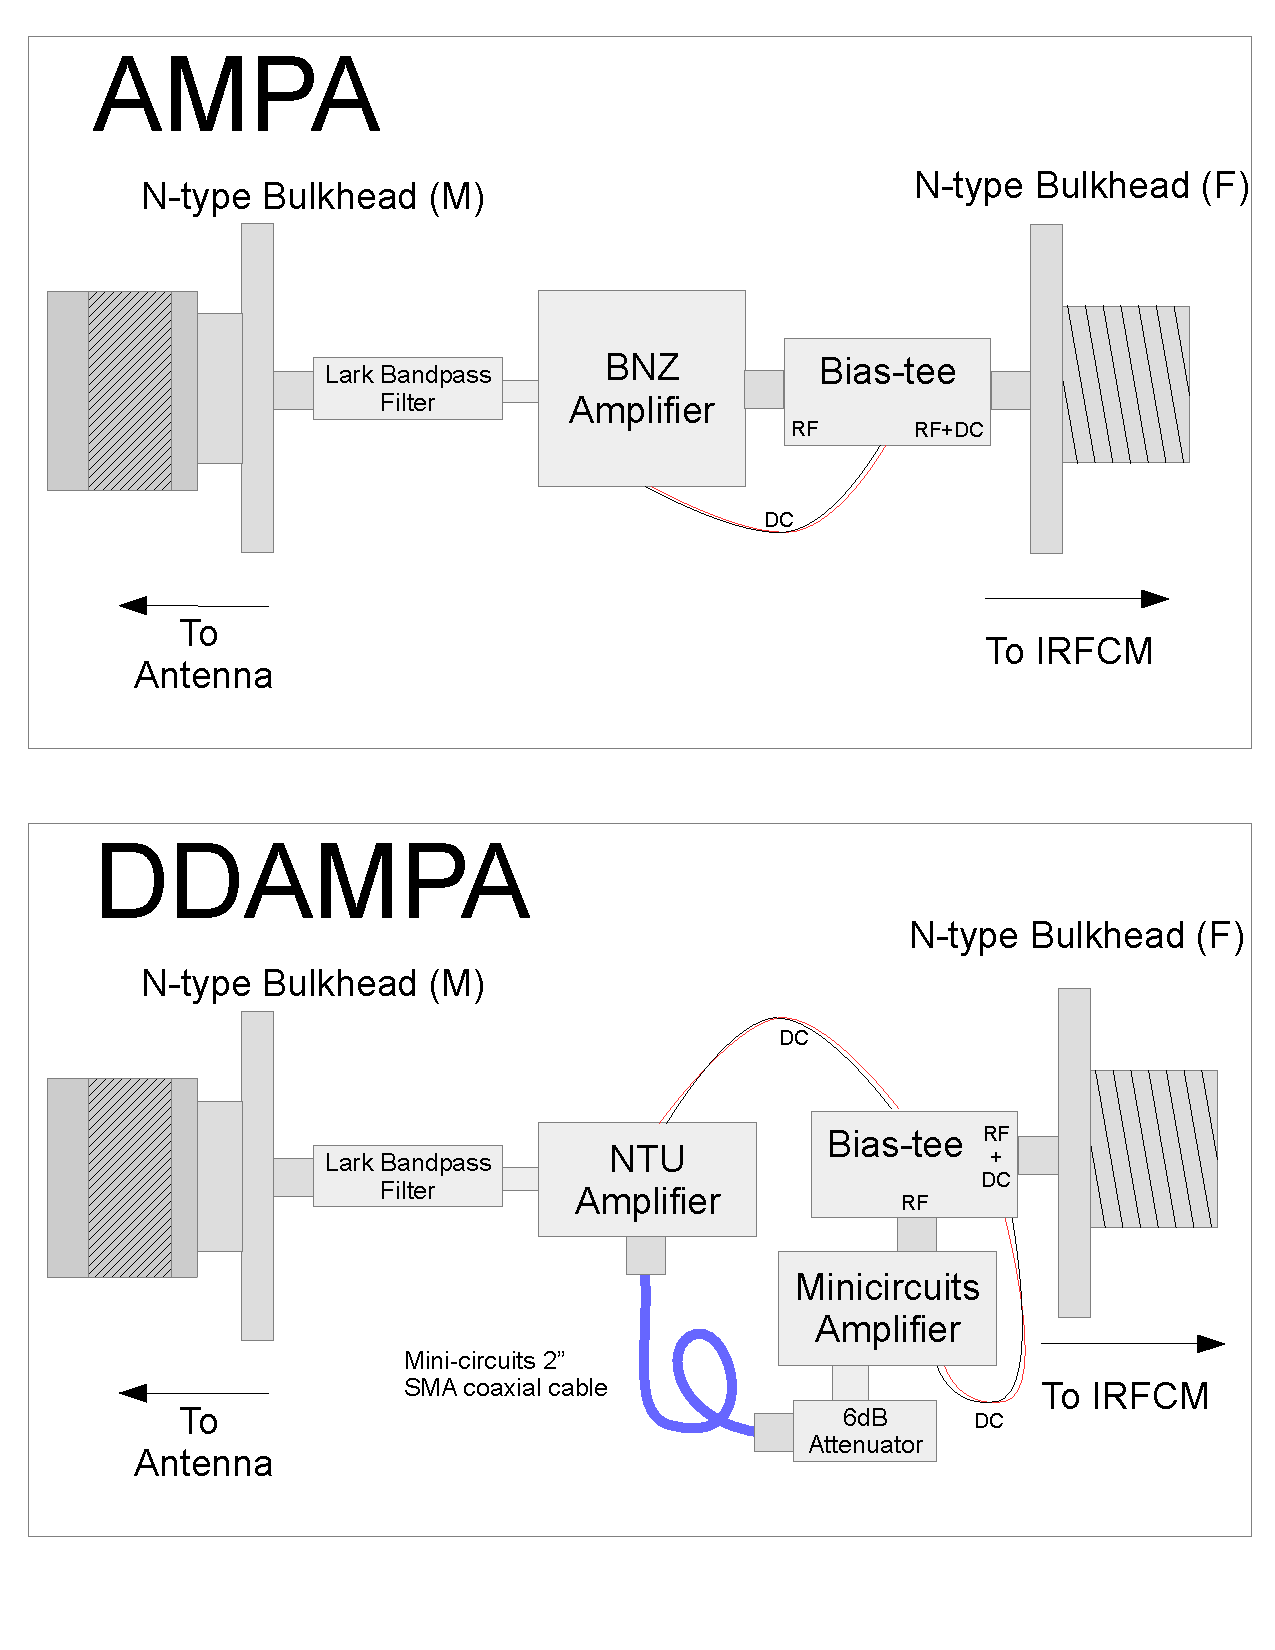
\includegraphics[width=0.85\textwidth]{figures/AmpaDDampaBlock}
	\caption{Block diagram for AMPA and DDAMPA front end amplification units}
	\label{fig:AmpaDDampaBlock}
\end{figure}

\begin{figure}
\centering
	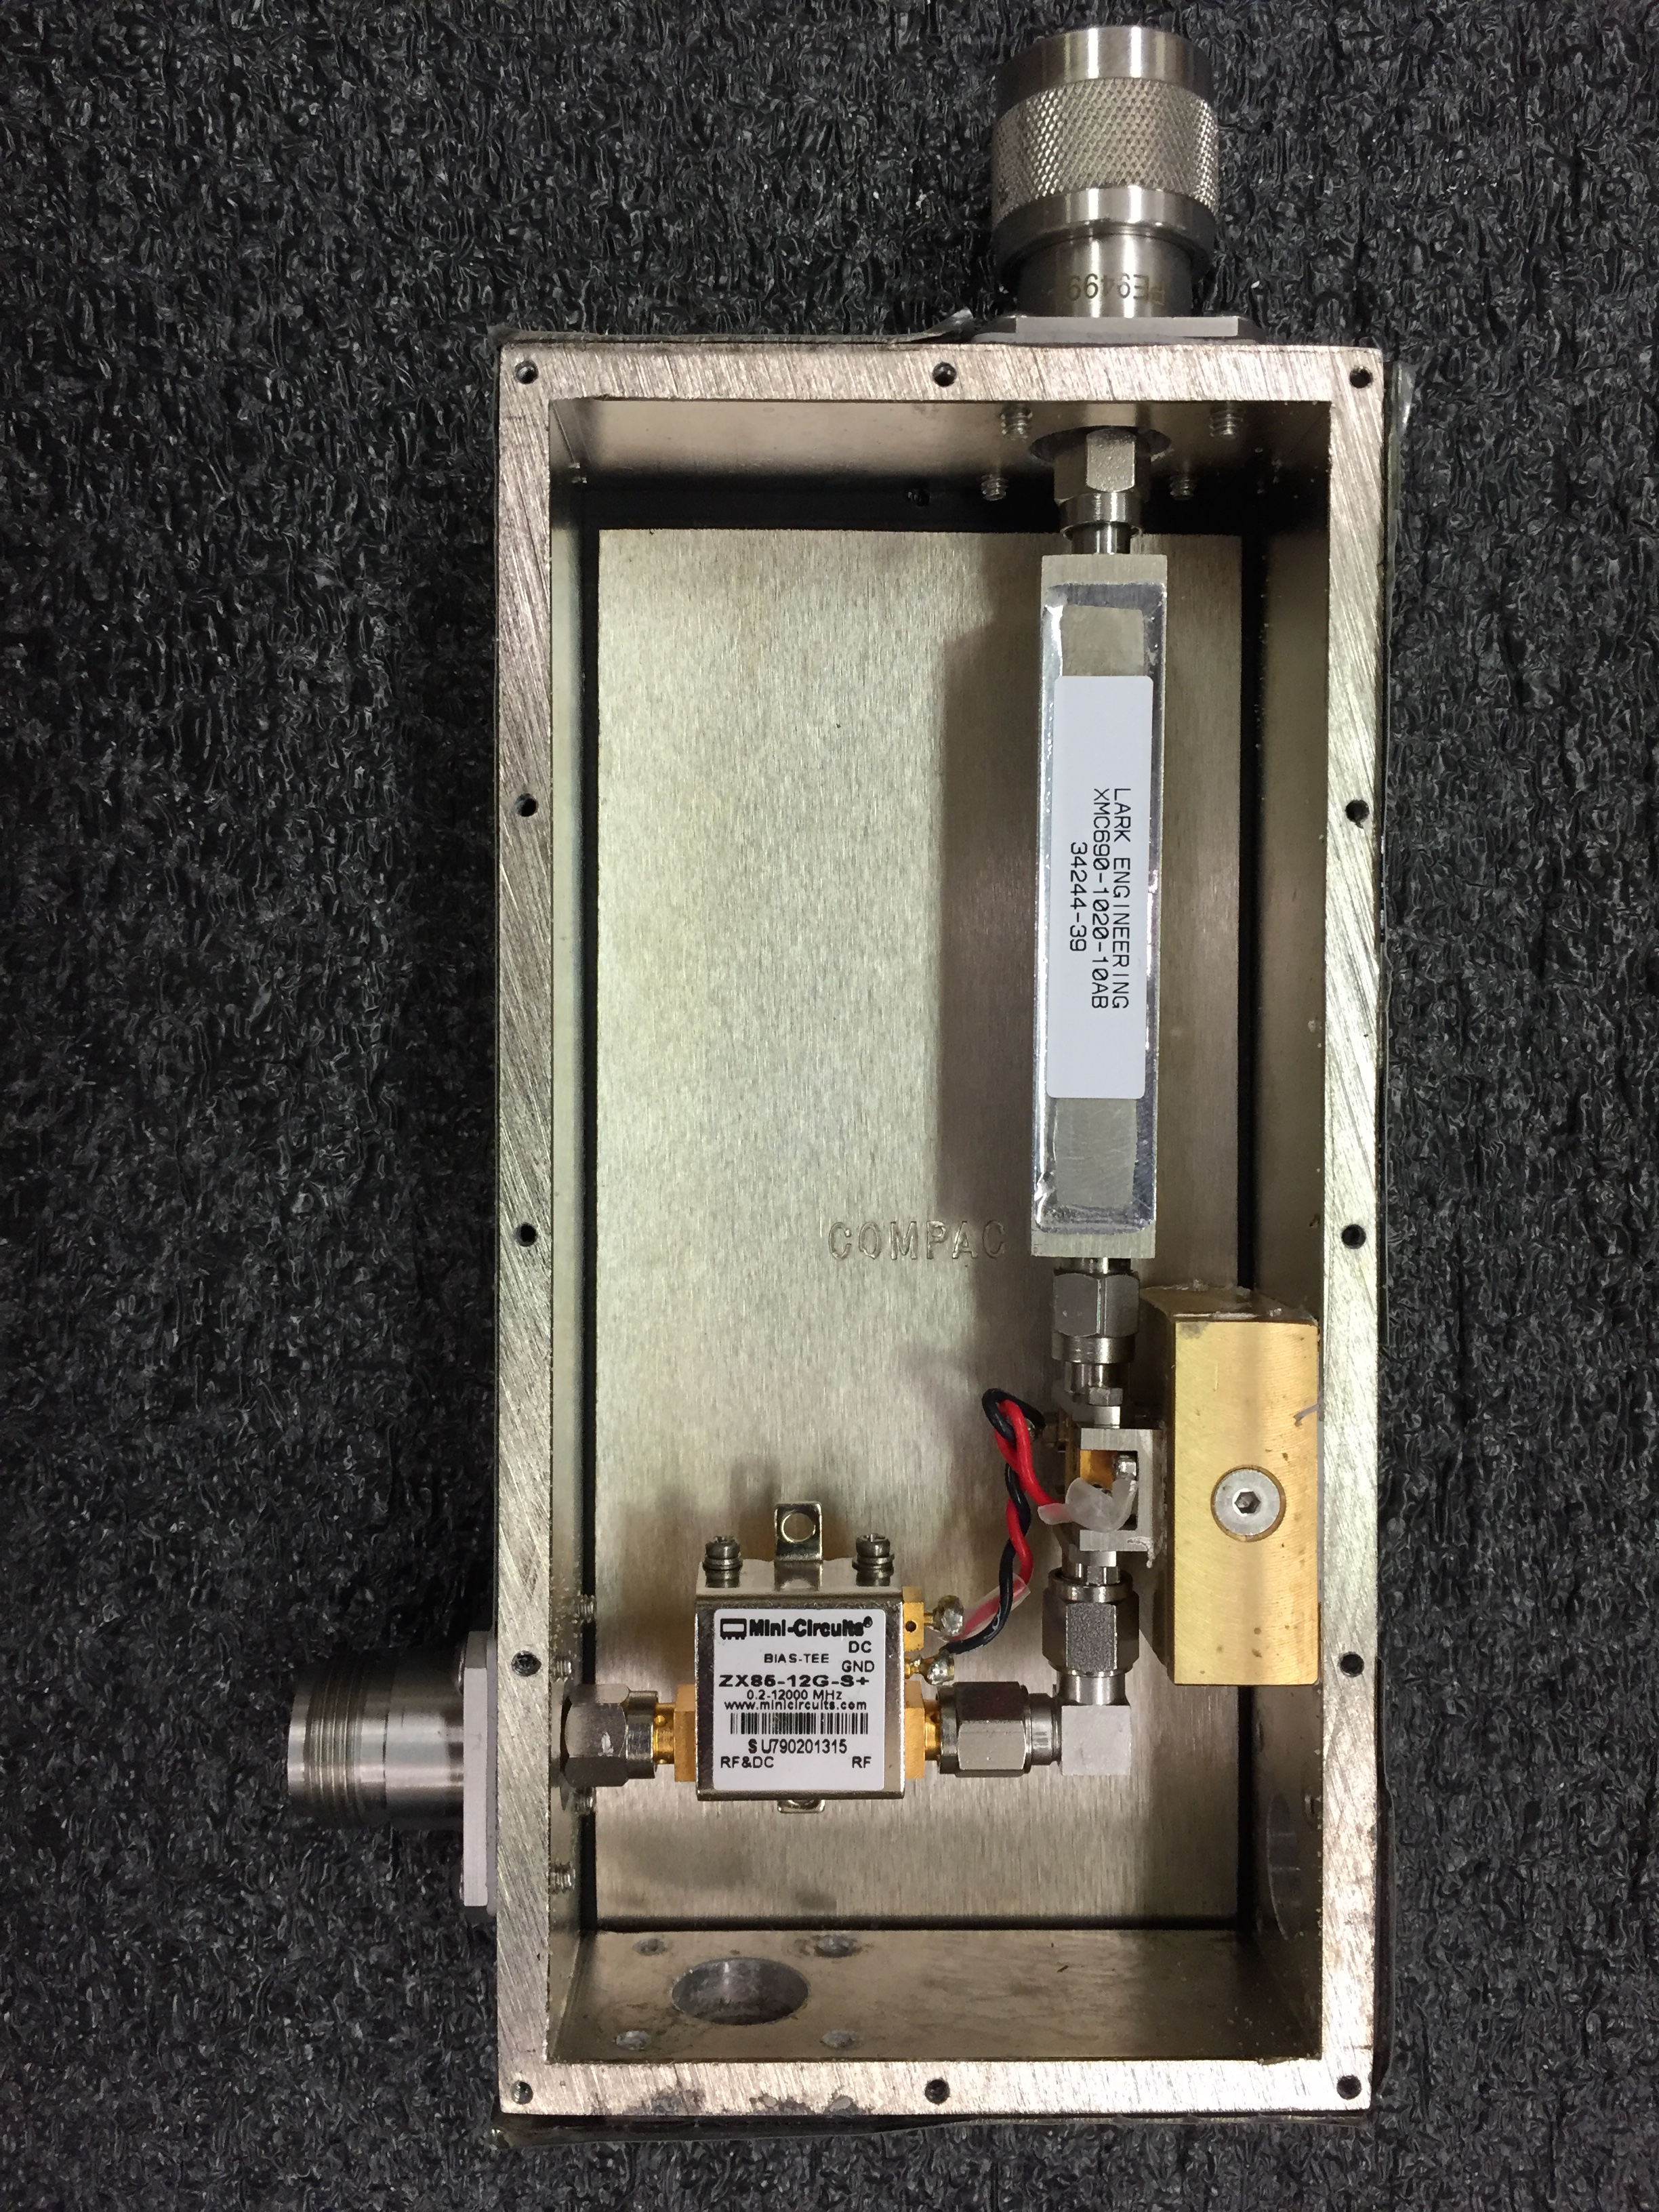
\includegraphics[height=0.45\textheight]{figures/AMPA}
	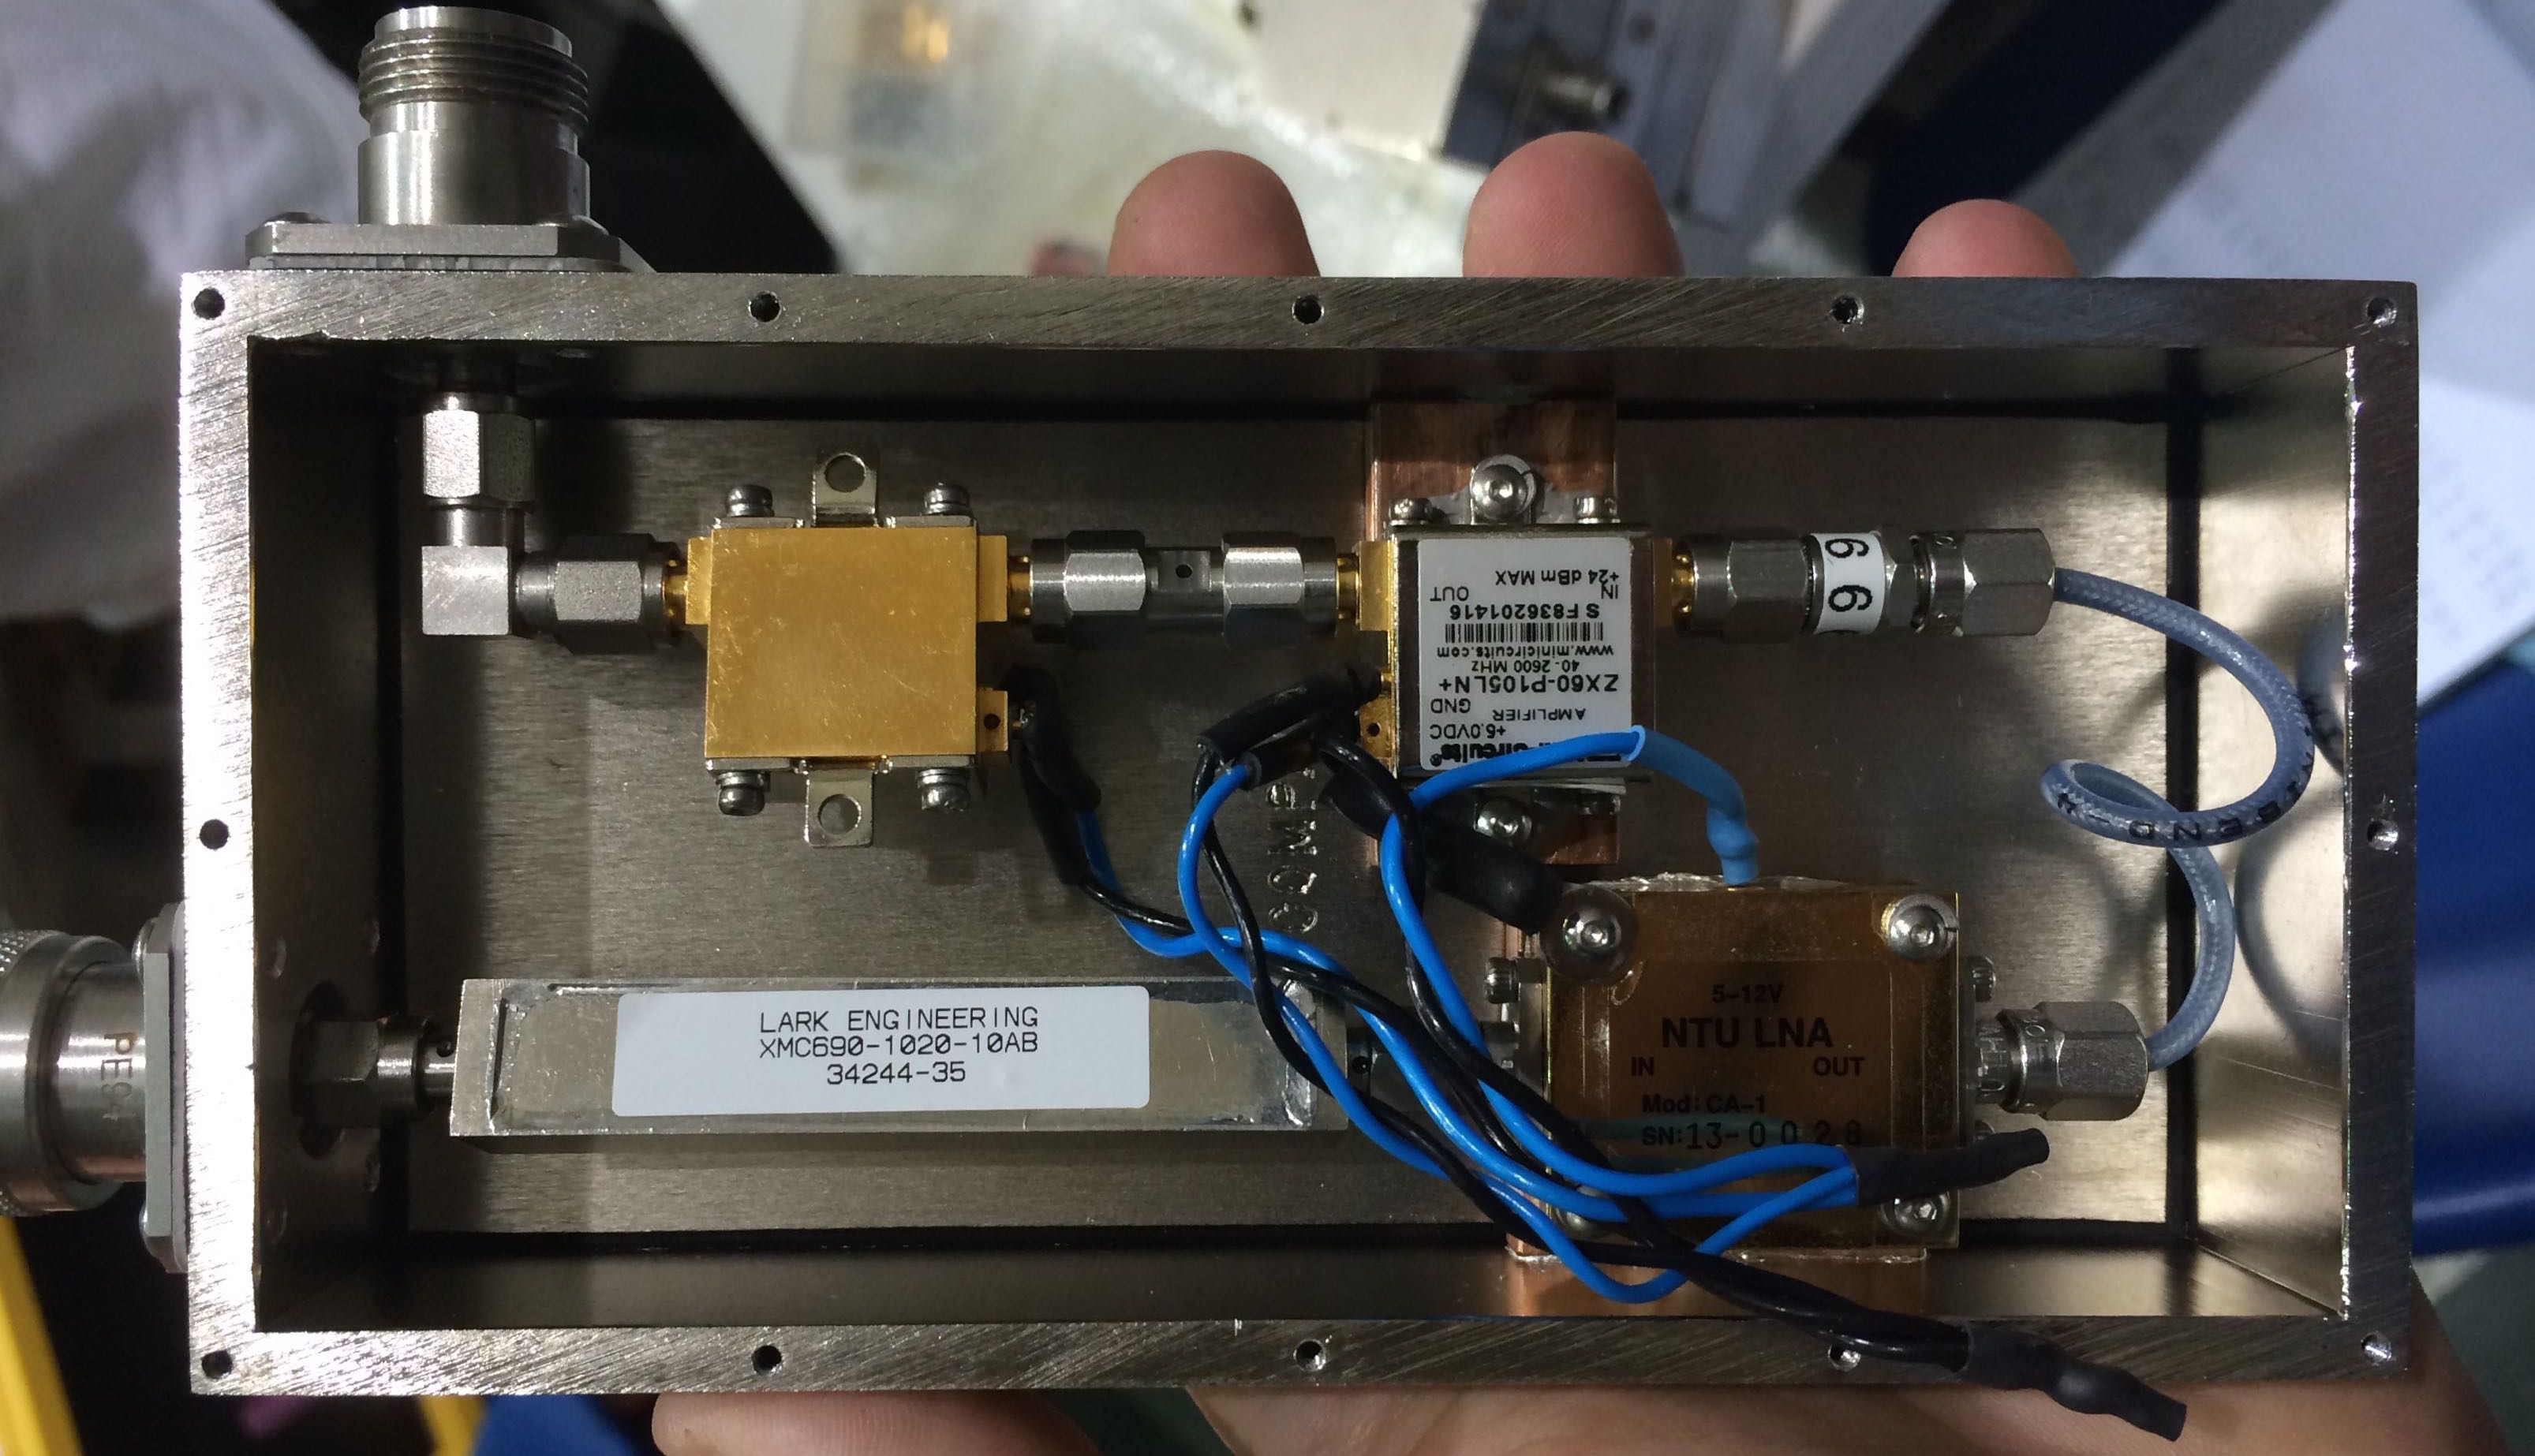
\includegraphics[height=0.45\textheight]{figures/DDAMPA}	
	\caption{The AMPA (top) and DDAMPA (bottom) internals.  AMPA photo courtesy of Jarred Roberts.}
	\label{fig:AMPAandDDAMPA}
\end{figure}	

\begin{figure}
\centering
	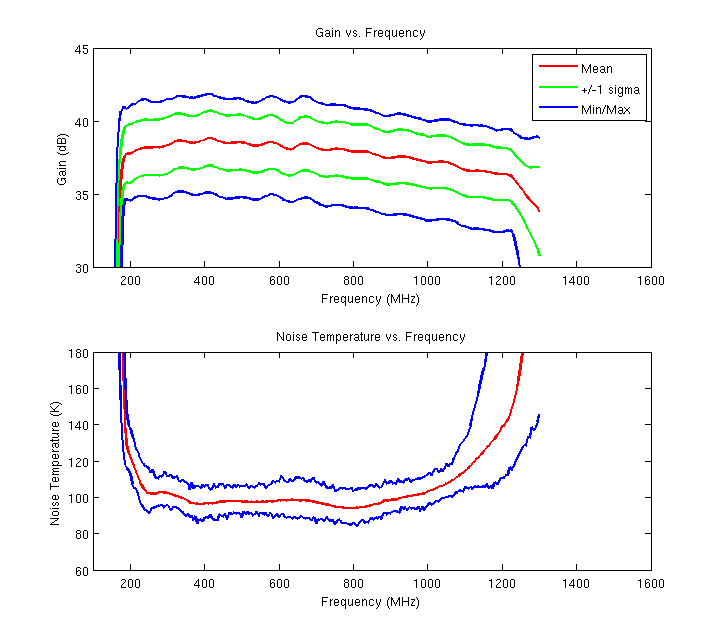
\includegraphics[height=0.45\textheight]{figures/ampas_std}
	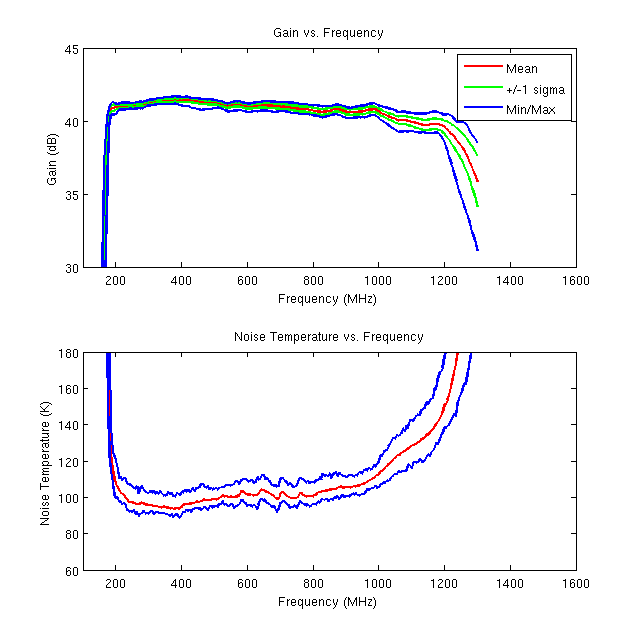
\includegraphics[height=0.45\textheight]{figures/ddampas_std}	
	\caption{Mean and standard deviation of gain and noise figure measurements for the AMPA (top) and DDAMPA (bottom) amplifier modules, as reported within ANITA}
	\label{fig:AMPAandDDAMPA_std}
\end{figure}	
	
	\subsection{iRFCM}
	The four custom built Internal Radio Frequency Condionting Modules (iRFCM), the internals of which can be seen in figure \ref{fig:IRFCMpic}, handle second stage amplification and bias network supply for 24 of the RF signal channels.  The block diagram for a single iRFCM channel is presented in Figure \ref{fig:IRFCM}.  There are three major active RF components for each signal chain present within the module. The AmpLite, a high gain, high dynamic range amplifier built by Patrick Allison of OSU, a tuning attenuator for gain balancing of the 96 different channels, and a bias-tee which, as its name suggests, adds a DC bias to the center conductor of the coaxial transmission cable between the AMPA and the iRFCM.  This bias is used to power the AMPA and DDAMPA amplifier modules.  The power gain for all 96 iRFCM channels is shown in Figure \ref{fig:IRFCMgain}.

\begin{figure}
\centering
	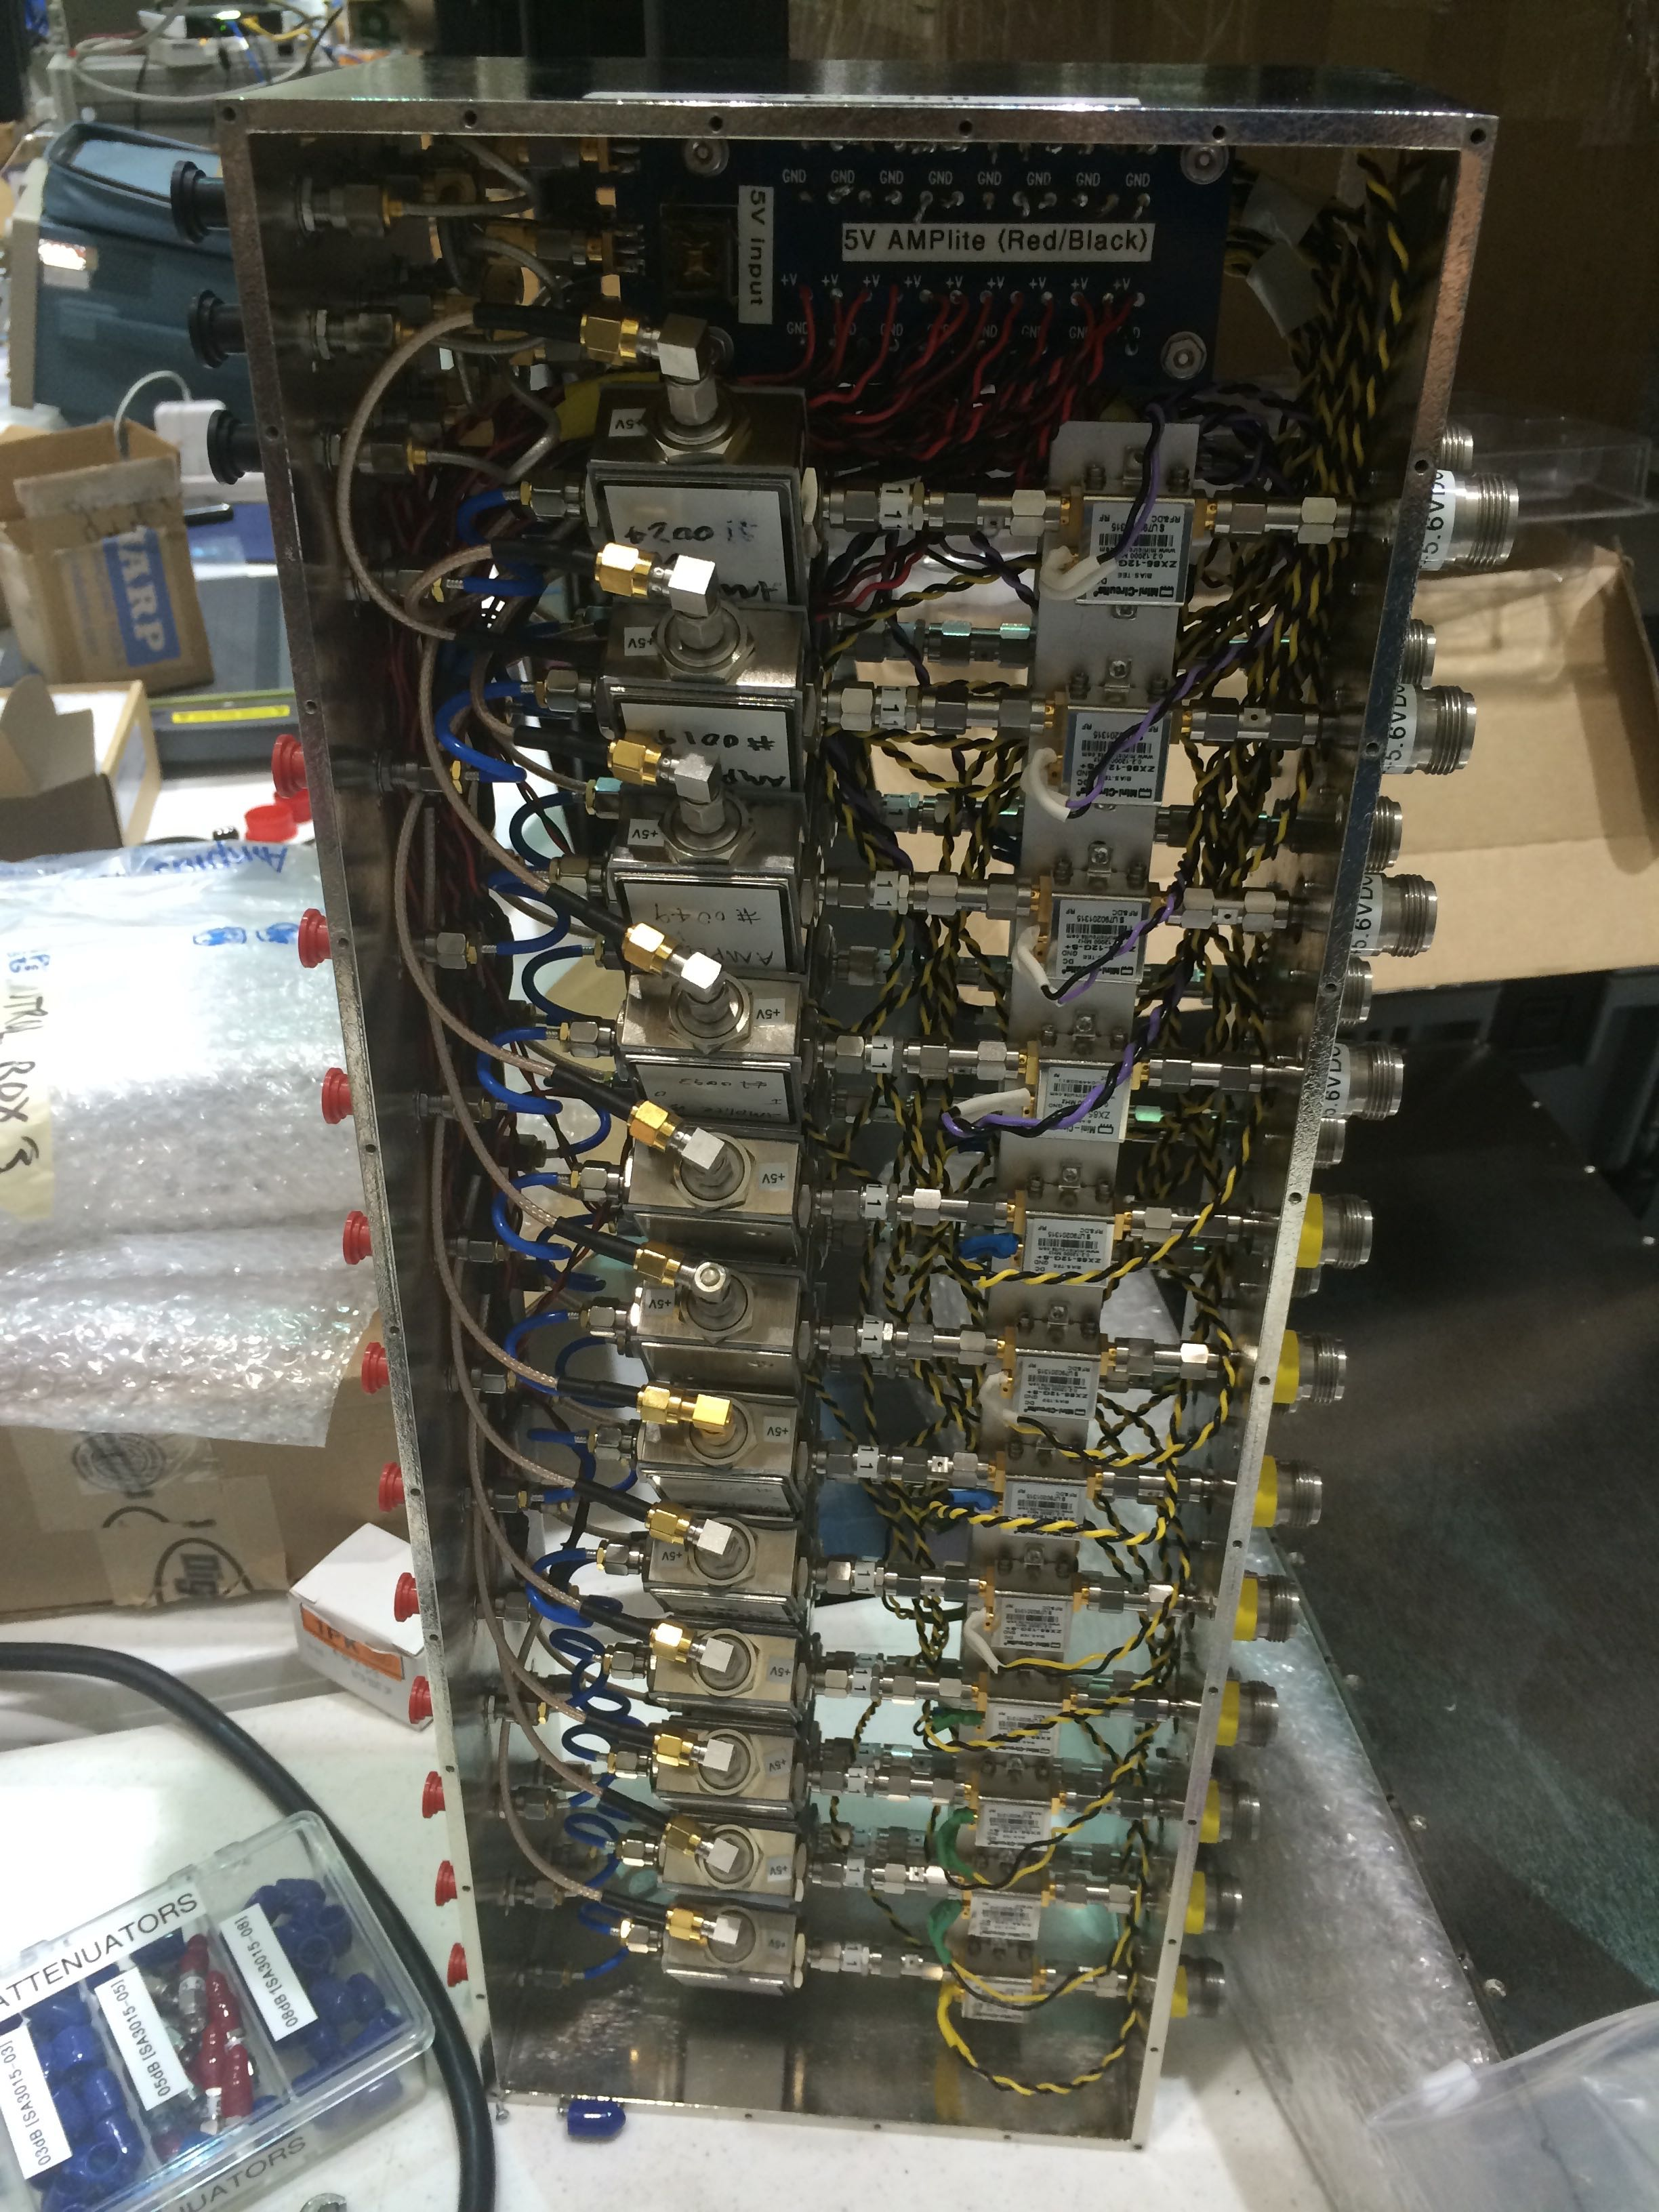
\includegraphics[height=0.9\textheight]{figures/IRFCMpic}
	\caption{An image of the internals of an iRFCM module after assembly}
	\label{fig:IRFCMpic}
\end{figure}

\begin{figure}
\centering
	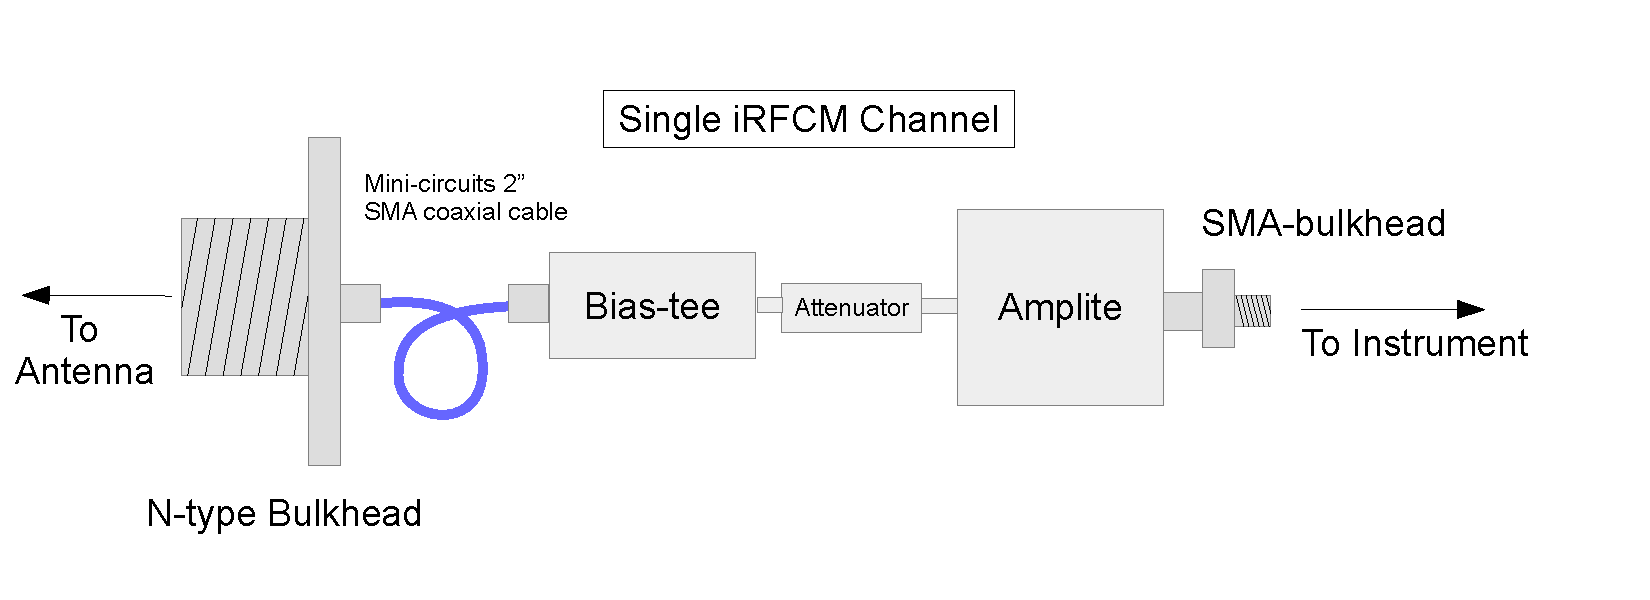
\includegraphics[width=\textwidth]{figures/IRFCM}
	\caption{A block diagram of a single iRFCM RF channel.  The bias-tee, as its name suggests, adds a DC bias to the signal in order to power the pre-amplifier modules.}
	\label{fig:IRFCM}
\end{figure}
	
\begin{figure}
\centering
	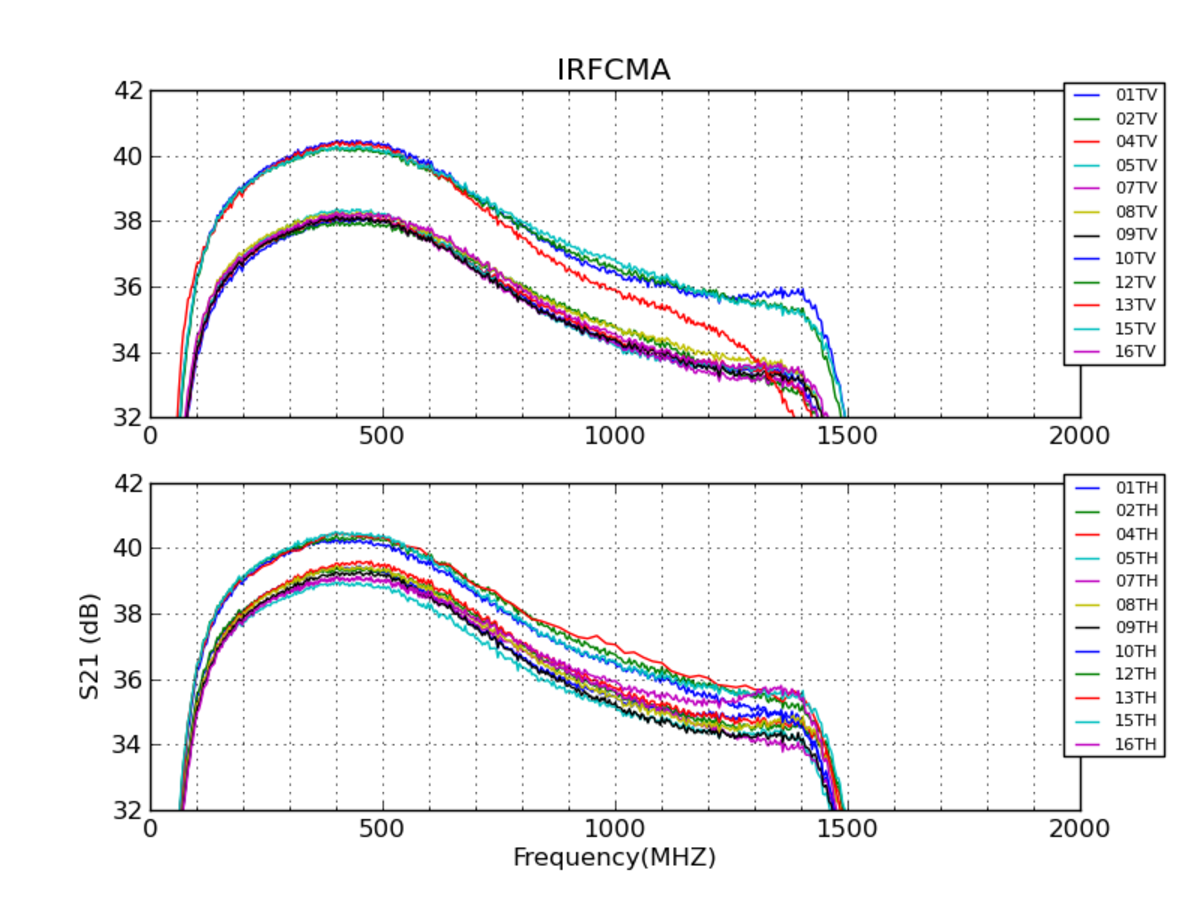
\includegraphics[width=0.45\textwidth]{figures/IRFCMA}
	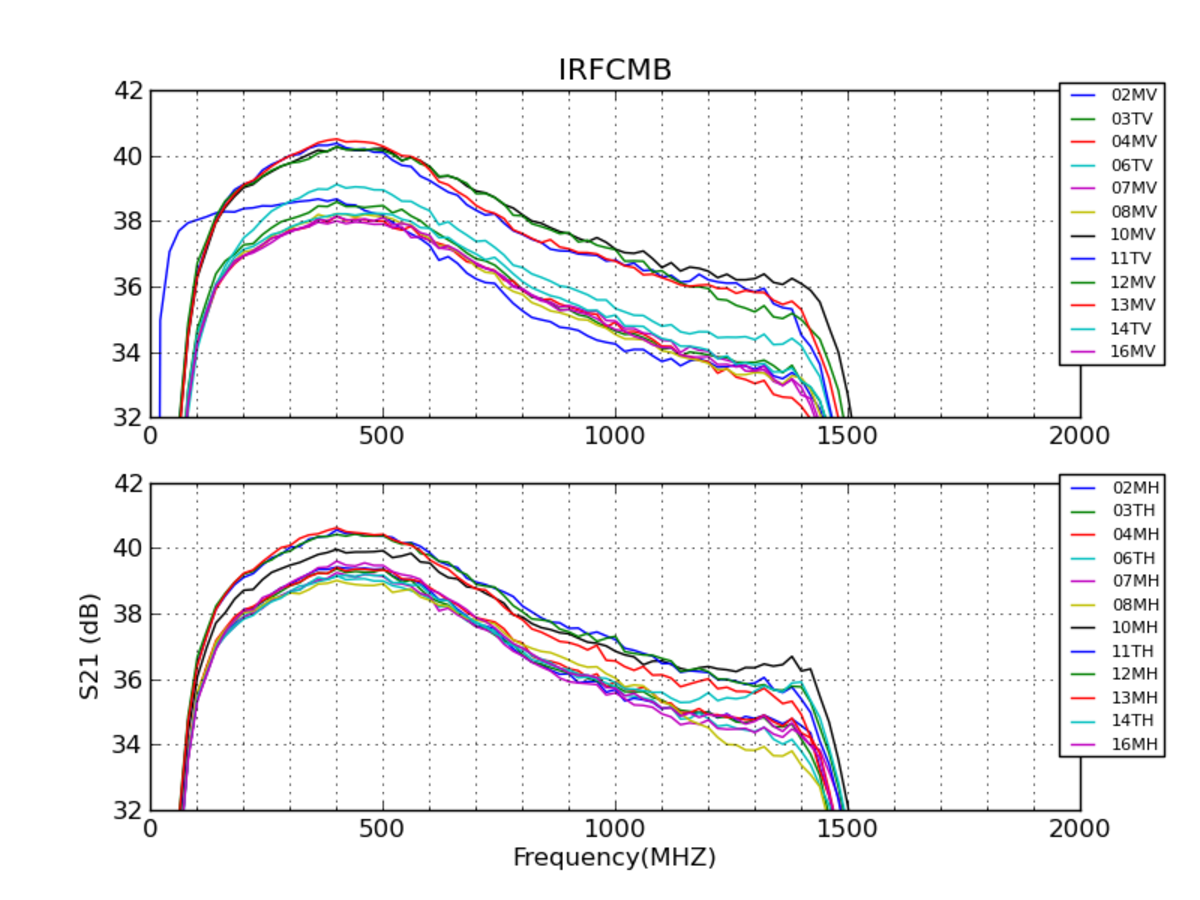
\includegraphics[width=0.45\textwidth]{figures/IRFCMB}	
	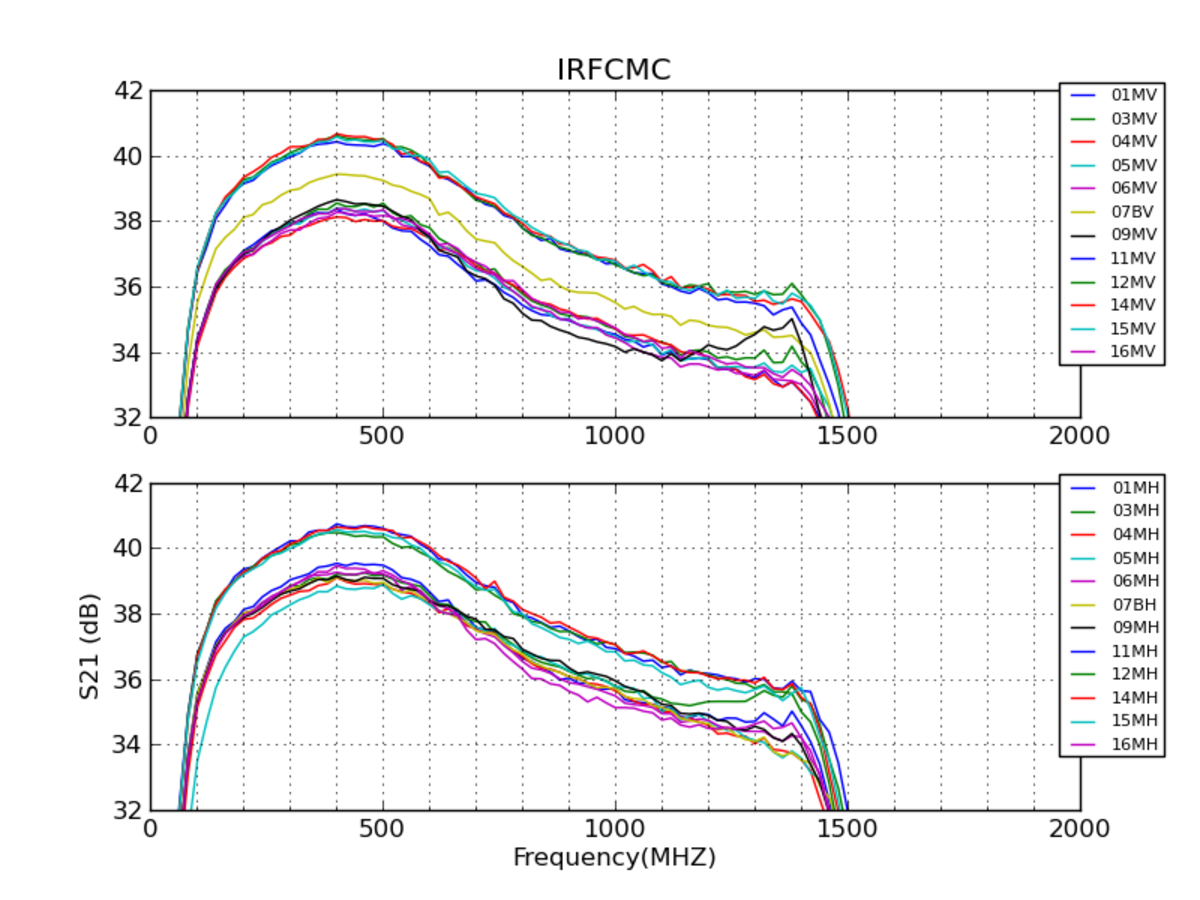
\includegraphics[width=0.45\textwidth]{figures/IRFCMC}
	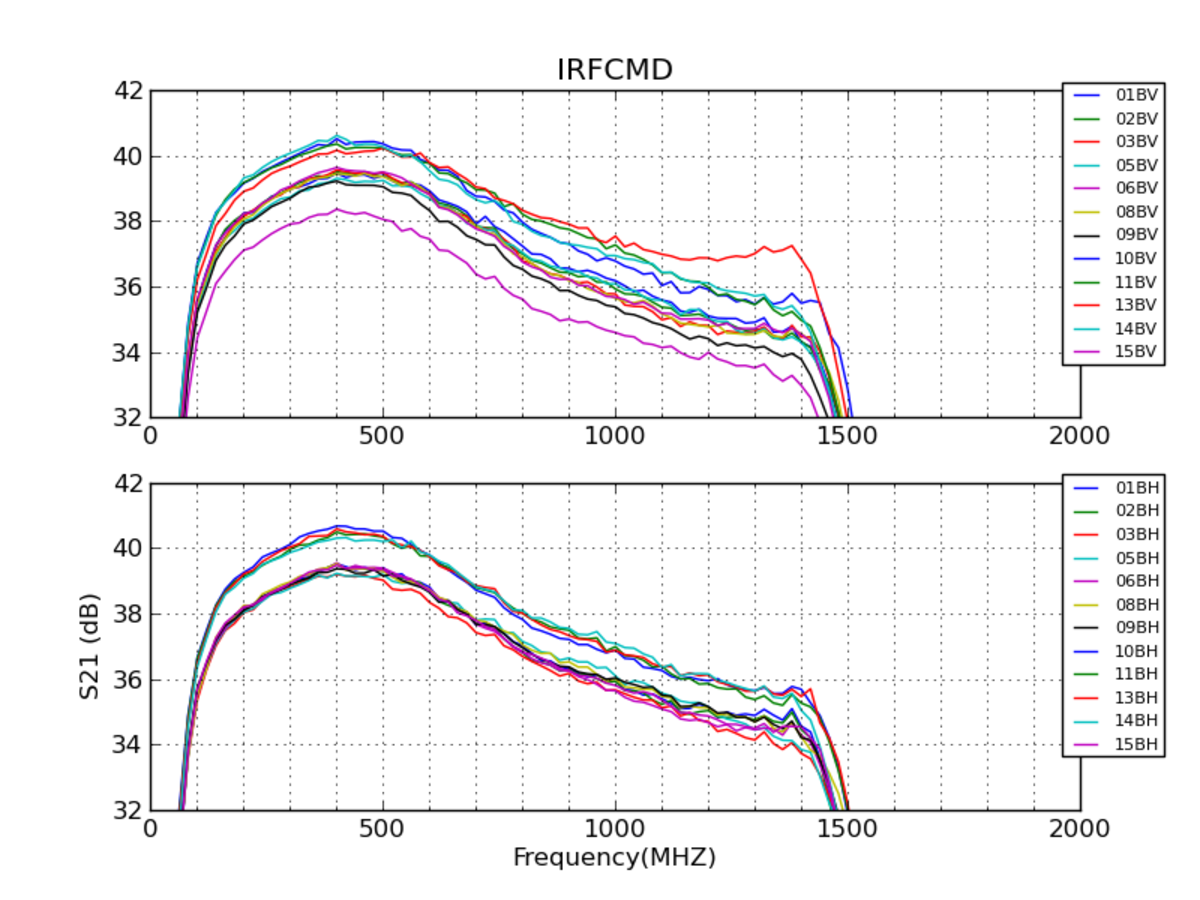
\includegraphics[width=0.45\textwidth]{figures/IRFCMD}	
	\caption{Gains for all 96 iRFCM channels.  The two distributions are intentional, used to equalize for the differences in gain between the AMPA and DDAMPA electronics. iRFCM channels were paired with specific pre-amplifier modules to equalize total system gain across all channels.}
	\label{fig:IRFCMgain}
\end{figure}		

	\subsection{Expected electromagnetic field variations}
		Depending on the radiation mechanism being observed, the power of an EAS signal measurable at the detector is proportional to the energy of the incident cosmic ray particle\cite{EnergyEstimator}.  This is shown in Figure \ref{fig:EASSignalPower} This signal power is convolved with the thermal and anthropogenic antenna noise present within the field of view of the detector.  The constant thermal emission of matter in the field of view of an antenna introduces a Johnson-Nyquist thermal noise component, which is calculated in Equation \ref{eqn:NyquistNoise},

\begin{equation}
	\label{eqn:NyquistNoise}
	P = k_{b}TB
\end{equation}

\noindent where $P$ is the thermal noise power observed across a termination resistor in Watts, $k_{b}$ is Boltzmanns constant, $T$ is the absolute temperature observed temperature in Kelvin, and $B$ is the frequency bandwidth in Hz.  The antenna, creating a smooth transition between the impedance of free space and that of the coaxial transmission network, has a noise temperature dictated by the integral of the temperature of objects in its field of view $(T(\theta,\phi))$, weighted by the gain pattern of the antenna $(G(\theta,\phi,\omega))$, as shown in equation \ref{eqn:antTemp}.

\begin{equation}
	\label{eqn:antTemp}
	\int_{-\pi}^{\pi}\int_{\theta}^{2\pi}\int_{0}^{\infty} G(\theta,\phi,\omega)*T(\theta,\phi)sin^{2}\theta d\theta d\phi d\omega
\end{equation}


\begin{figure}
\centering
	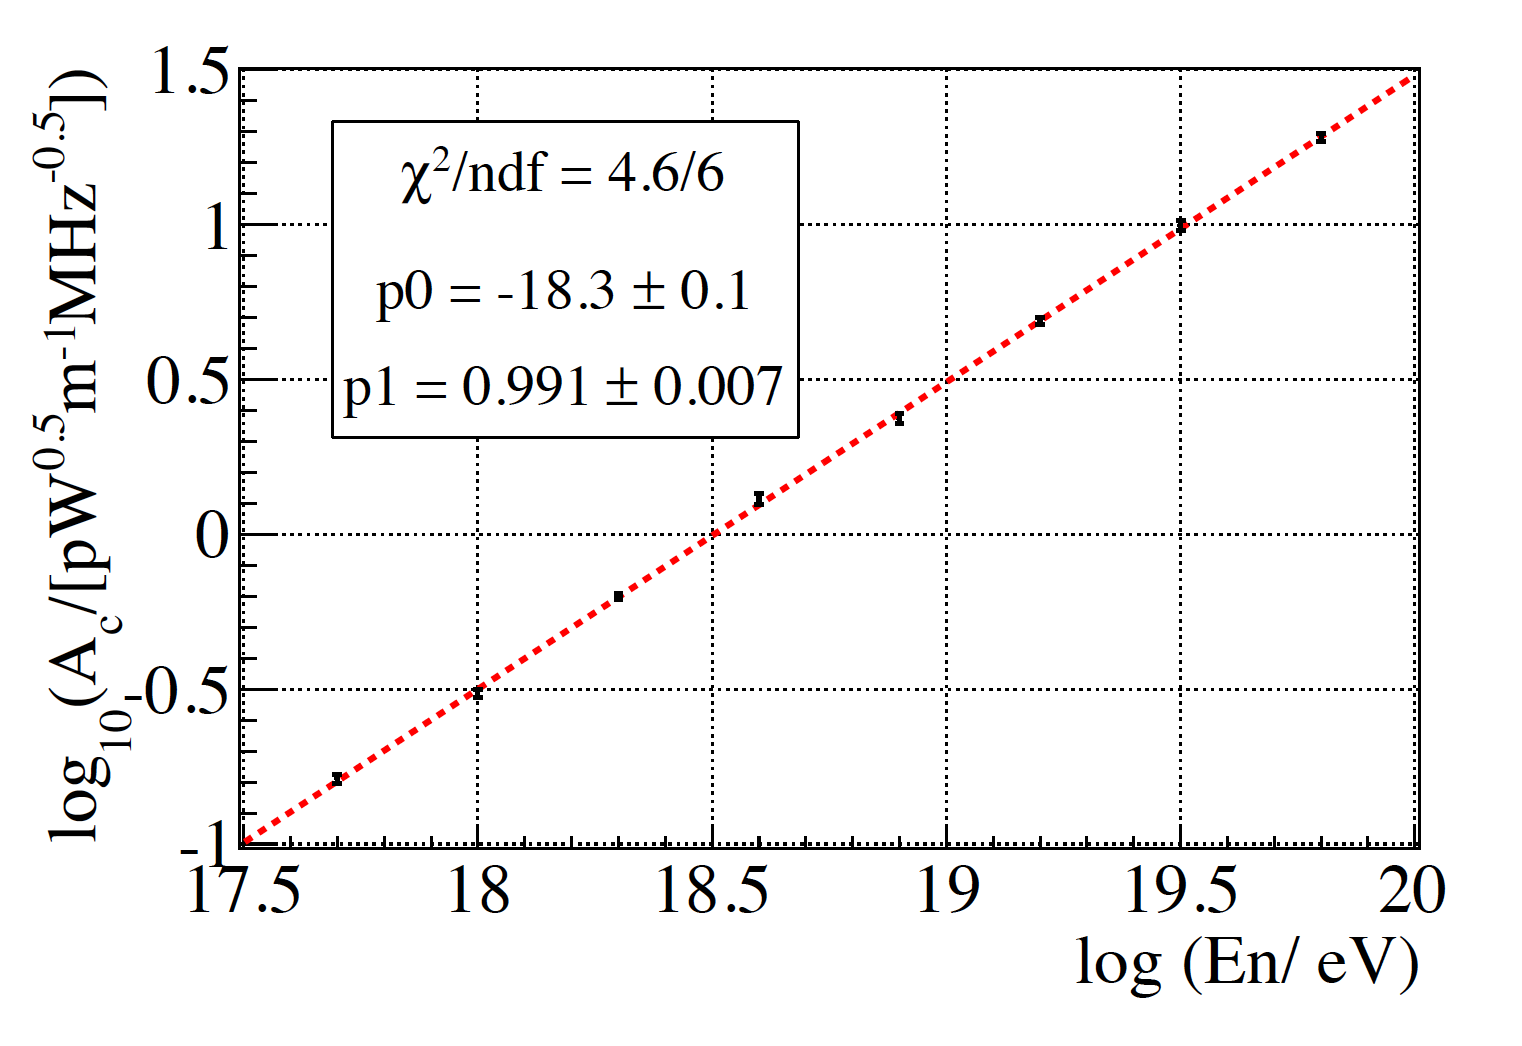
\includegraphics[width=\textwidth]{figures/EASSignalPower}
	\caption{The relationship between EAS signal power at the peak coherence angle and primary particle energy, from \cite{EnergyEstimator}.}
	\label{fig:EASSignalPower}
\end{figure}

	\subsection{Noise Figure} 
	Since amplification is required, a minimum of additional electronics noise introduced by the detector.  Besides a background of thermal noise, the dominant continuous noise source is electronics noise from the amplifiers. This noise, unlike the thermal noise incident on co-pointing antennas, is not coherent as each amplifier adds its own uncorrelated noise component.  The noise figure is additionally increased by any loss of power in front of the amplifiers.  Since the noise figure cascades through an amplifier chain, it is imperative to reduce any additional noise figure at the beginning of the signal chain, and less important in the subsequent amplifiers.  The cascading noise can be calculated using Frii's Formula (Equation \ref{eqn:noiseCascade}), where $T_{total}$ is the resulting noise temperature of the entire signal chain, $T_{n}$ is the noise temperature of a specific element, and $G_{n}$ is the gain magnitude of a specific element.
	
\begin{equation}
	\bar{v}^{2} = 4k_{b}BRT
	\label{eqn:JohnsonNyquistNoise}
\end{equation}

	
\begin{equation}
	\label{eqn:noiseCascade}
	T_{total} = T_{1} + \frac{T_{2}}{G_{1}} + \frac{T_{3}}{G_{1}G_{2}} + ... + \frac{T_{n}}{G_{1}G_{2}...G_{n-1}}
\end{equation}
	
	From this, one can see that the +38dB of gain from the first stage amplifier reduces any subsequent noise figure from components by a factor of $38dB = 10*log(G) \rightarrow 10^{38/10} =  6309 = G$, alleviating the requirement for low noise amplifiers in subsequent stages.


	\subsection{Dynamic Range and Gain}
		Each instrumental system measuring the electromagnetic field operates at a different optimal power level.  For example, the digitizer ASIC can cover an approximately 2V full dynamic range.  An observed voltage with peak to peak amplitude significantly below that level would never exercise the full range of the digitizer and allow bit level digitizer noise to become dominant over the antenna noise background.  Equally and oppositely, too high an input power signal would become distorted at high peak amplitudes, as near full scale voltages the response of the digitizer becomes nonlinear, or "compressed". 
		
		There are three systems measuring the signal on the coaxial feed line from the antenna, which will be discussed in detail later: the LABRADOR digitizer, the tunnel diode before the trigger circuit, and a broad spectrum RF power monitor.  The required gain of the system can be arrived at by determining their input power range, then calculating what amplification of expected signal is required so that the power sits within that specification.  The total system gain is driven by the instrument that requires the highest power, and any instruments that require lower input power are given in-line, flat spectrum, fixed attenuator components.  Table \ref{tab:rfLinkBudget} contains the three terminal components, their dynamic ranges, and the required gain necessary to put observed thermal noise from the antenna into a measurable power region.  The justification for components not yet mentioned in this thesis are covered in subsequent sections in this chapter.
	
\begin{table}
	\centering
	\begin{tabular}{| l | c | c |}
		\hline
		Component & Maximum Power & Gain Requirement\\
		\hline
		LABRADOR digitizer & 20dBm & 80dB \\
		RF Power Monitor & -10dBm & 50dB \\
		SHORT and Tunnel Diode & 0dBm & 60dB \\
		\hline
	\end{tabular}
	\caption{A description of the required input power and gain requirements for the three terminal instrumentation components of the ANITAIII system}
	\label{tab:rfLinkBudget}
\end{table}
	


	
\section{Digitization}
	The dynamic electromagnetic field variations incident on the payload are digitized using an array of custom designed fast analog to digital converter (ADC) application specific integrated circuits (ASICs).  The ANITAIII instrument utilizes the third iteration of the LABRADOR (Large Analog Bandwidth Recorded And Digital Ordered Readout), the LAB3, designed by Gary Varner\cite{LABASICPAPER}.  This chip was used on the first three ANITA flights because of its high precision, large dynamic range, Gigahertz of analogy bandwidth, and extremely low power requirements.   It is a 12-bit, 2.6GS/s, ~256 sample long ADC, yielding a window size of ~100ns.  Each chip has 9 channels, consisting of 8 RF analog inputs, as well as a 9th global clock channel propagated to all LAB chips for alignment.  The SURF (Signal Unit for Radio Frequency) Board consists of 4 LABRADOR chips in order to allow multi-hit buffering, as well as paths for the trigger signal to a Field Programmable Gate Array (FPGA), discussed later.

	\subsection{LABRADOR3 ASIC}
	The LAB3 converts the analog signals to digital values through means of a sample and hold switched capacitor array read out with a wilkinson clock comparing the stored charge in a storage capacitor against a ramp signal driven by a constant current source.  The sampling time base is driven by a square pulse that propagates through a starved transistor array internally to the chip, toggling each capacitor sequentially.  This continuous sampling is halted when a trigger is formed and a HOLD is issued to the chip. The LAB3 is  Wilkinson ADC, which measures the time to threshold of a constant current voltage ramp and converts the stored charge in each capacitor to a digital value, then read out in parallel to an FPGA for further storage (see Figure \ref{fig:LAB_Dig}.  The time to threshold circuit uses a 100MHz clock and a Gray code counter.  Due to the dead time related to the digitization process, four LAB3 chips are placed in parallel in order to allow for multi-hit readout capabilities.  When a HOLD is issued, the LAB3 chip returns both an estimate of which RCO phase it is in (which due to propagation latency is inverted near the wraparound region), as well as the locations of the "HitBus", or samples that were left in tracking mode (connected to the RF input) when sampling was halted. The procedure and results of calibrating this readout is detailed in the Calibration section.
		

\begin{figure}
\centering
	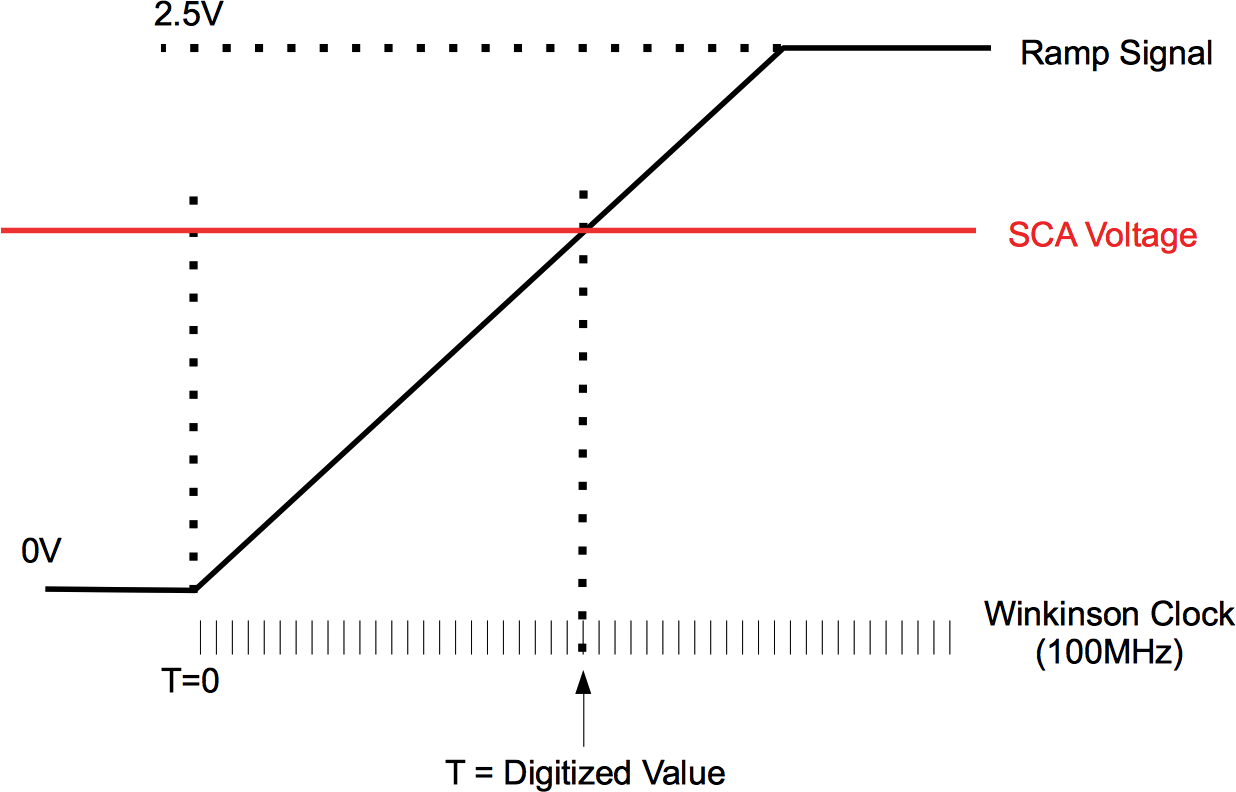
\includegraphics[width=\textwidth]{figures/LAB3_Dig}
	\caption{A simplified diagram of the LABRADOR digitization technique.  A linearly increasing voltage ramp signal is generated by driving a constant current into a set capacitance, which is compared versus the voltage present on each SCA capacitor.  At the beginning of the ramp signal, a 100MHz Wilkinson clock is started, which increments a 12 bit counter at every clock period.  At the time of the threshold crossing, the value is latched and read out as the digitized value.}
	\label{fig:LAB_Dig}
\end{figure}

		
\begin{figure}
\centering
	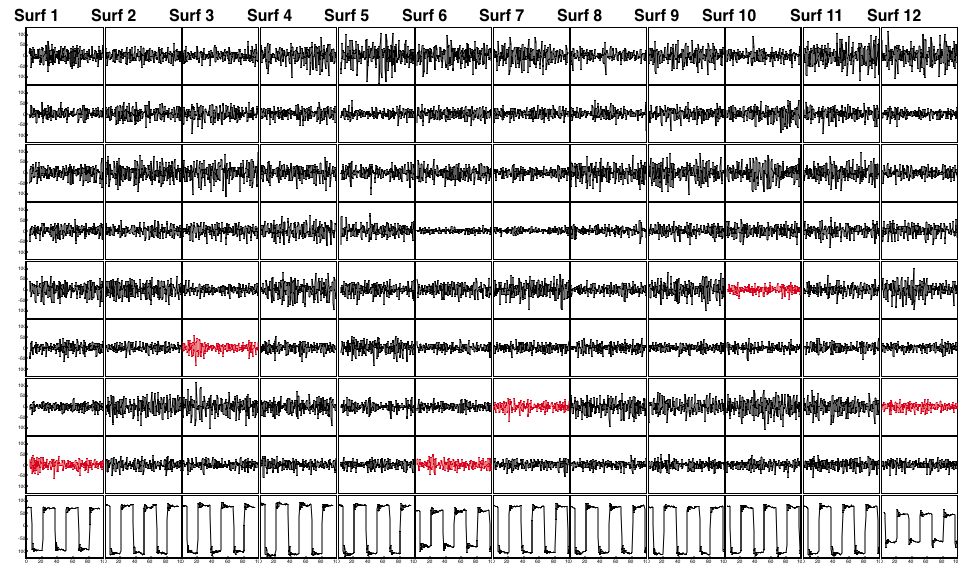
\includegraphics[width=\textwidth]{figures/waveformSnapshot}
	\caption{An example readout of all 96 channels of the full ANITAIII detector, organized by SURF (columns) and channels (rows).  Bottom row is the synchronization clock inserted into all LAB chips.  In red are phi sectors that triggered the event.  This particular waveform is low SNR, self-triggered, West Antarctic Ice Sheet (WAIS) calibration pulser (ev 61326092).  Image was made with MagicDisplay data visualization code.}
	\label{fig:waveformSnapshot}
\end{figure}
		
	
	
	\subsection{Limitations}
	After a hold is issued to a chip, the digitization freezes the ring buffer and yields the chip unable to sample until digitization is complete, a process that can take  many microseconds.  During a readout, no new data can be captured by the LAB3 chip.  To alleviate this, the RF input chain is split into four separate chips which are read out one at a time.  This provides a buffer depth of four, which allows the instrument to remain live even while reading out several concurrent events.
	
	The analog bandwidth of the LAB3B (used in the ANITAIII and ANITAII experiments) did not fully cover the full bandwidth of the antennas and signal chain, which yields a drop-off in sensitivity for high frequency signals.  The total system bandwidth is shown in the calibration Chapter, however a measurement of the analog bandwidth of the LAB3B specifically is shown in Figure \ref{fig:LAB3B_bandwidth}
	
\begin{figure}
\centering
    \textbf{LABRADOR3}\par\medskip
	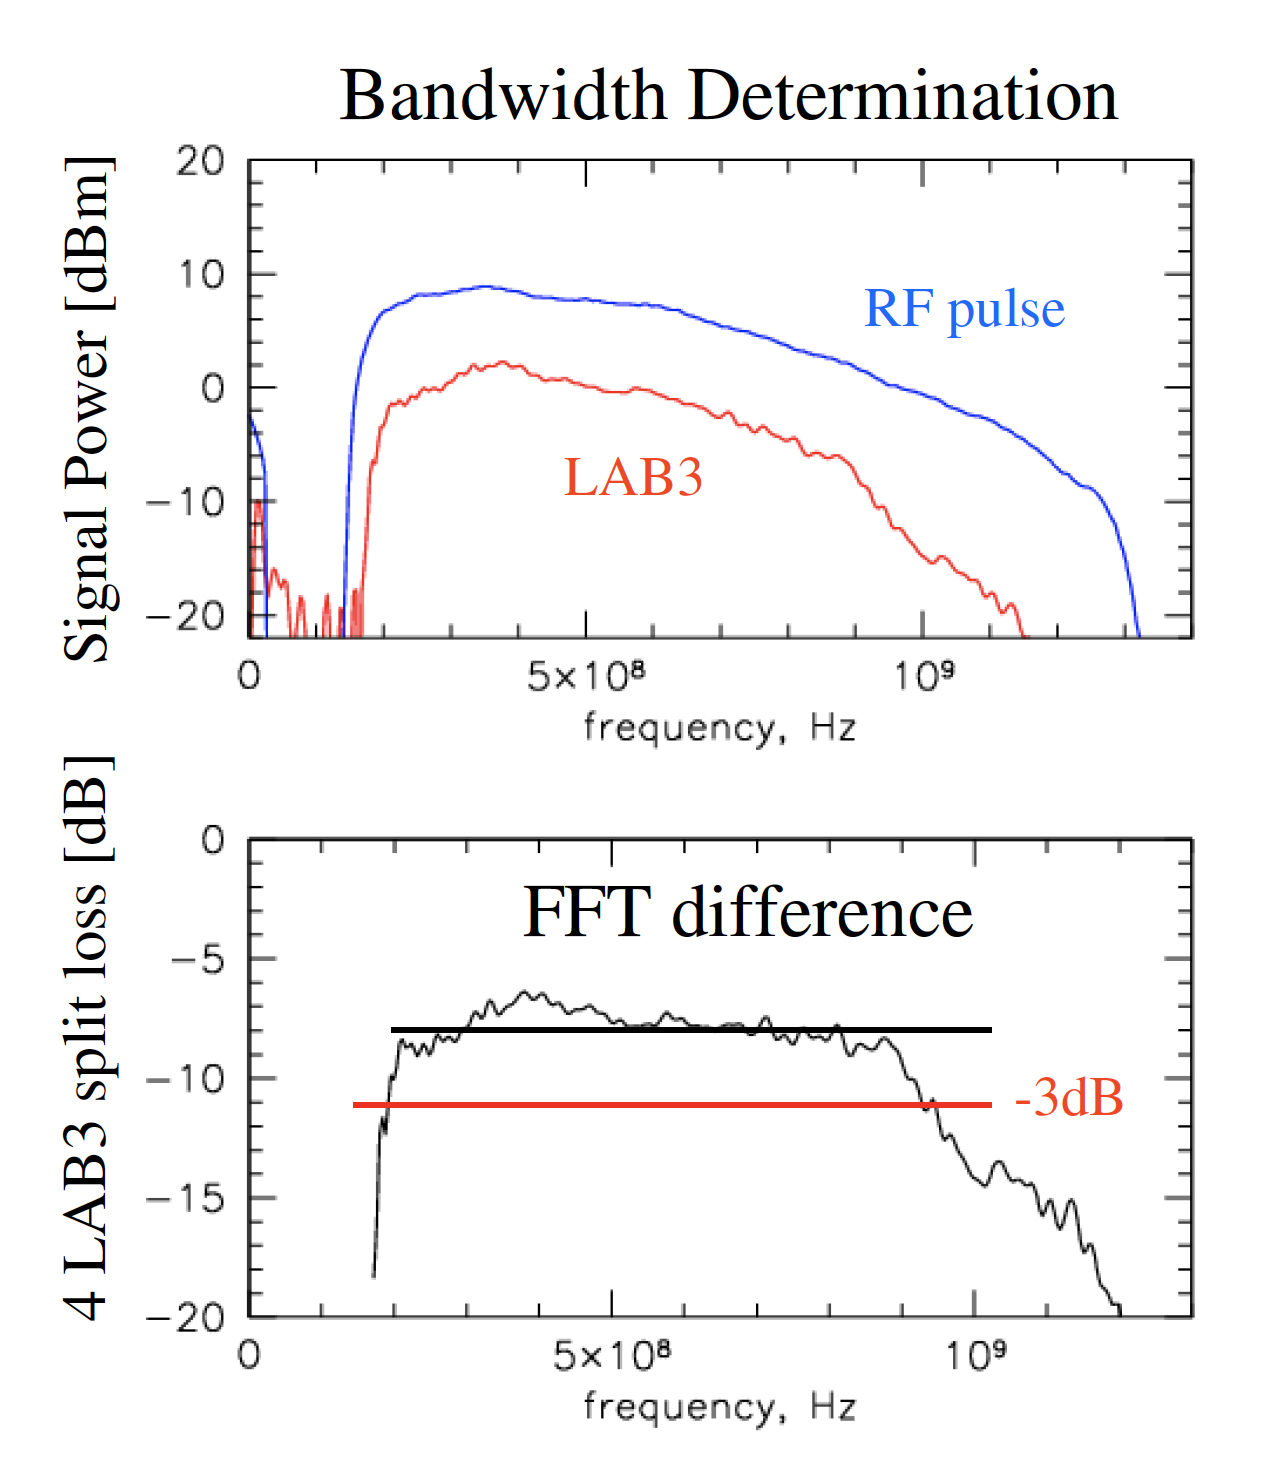
\includegraphics[width=0.8\textwidth]{figures/LAB3B_bandwidth}
	\caption{Bandwidth measurement of the LAB3 digitizer chip measured through injection of a impulsive signal to a test board.  The signal undergoes a 4-way split on the test board to emulate the SURF board.  In the top figure, the spectral power of a (blue) RF reference pulse and (red) LAB3 readout pulse are shown. At bottom is the difference, where a -6dB board loss would be expected with perfect coupling(black line). The -3dB point occurs several hundred MHz below the 1.2GHz desired instrument high frequency limit.\cite{LABASICPAPER}  }
	\label{fig:LAB3B_bandwidth}
\end{figure}
	
	The time between samples is controlled by a charge starved transistor chain that controls the connection between the sampling capacitor and the input RF signal.  Due to process parameter spread in the manufacturing of the ASICs, the timing between subsequent samples is not well controlled.  This yields an uneven time sampling that needs to be corrected in calibration of each chip individually.  In addition, it leads to an unevenly sampled time domain waveform which introduces a difficult to correct frequency response, and requires interpolation between points before creating interferometric maps.  Interpolation is CPU intensive, an issue that makes doing in flight interferometry more difficult.
	
 	Since each LAB chip can only digitize eight channels concurrently, a total of twelve total SURF boards are required to measure all 96 channels of each event simultaneously.  The propagation of the readout HOLD signal from the FPGA, and its subsequent latching within each LAB, adds jitter that needs to be corrected in analysis.  The ninth channel on each lab observes a single 33.3MHz analog clock signal propagated through the CPCI backplane to each SURF.  By measuring the relative phase of this clock between SURFs, this jitter can be corrected for interferometry.  This is discussed further in the Calibration section.
 	
 	 Additionally, the 100ns SCA buffer length  limits the minimum full period oscillation observation frequency to 10MHz, however this is below the antenna frequency cutoff.  The effect of the limited trigger window is however visible in the ALFA low frequency antenna.
	
	\subsection{Impulse Response}
	The filtering and amplification chain has a dispersive effect on the signal, which requires a calibration of the system impulse response in order to fully understand the incident electromagnetic field.  An impulse response is the phase and gain distortion created by the RF network to an input signal.  In the ANITA, a band-limited system, the phase shift increases as a function of frequency, which causes the signal power to be spread temporally.  As a cross-correlation between multiple channels is dependent on the full complex parameters of the signal, significant variation between the impulse responses of channels will result in a reduced maximum correlation value, regardless of the electromagnetic impulse present at the antennas.  The ANITA instrument is designed to be identical and symmetric across all 96 channels, making this effect small and constant.  Measurements of this response and calibration are done in the Calibration section, and the effect and deconvolution is detailed in the Analysis section.

	
	\subsection{Future development}
	Since the LAB3 was developed in 2005, there has been significant development in the LABRADOR architecture.  The most advanced generation of chip, the LAB4D, is a single channel readout that improves upon the previous generations by both vastly increasing the storage buffer which increases the record length, or buffer depth of the chip.  It also allows for the correction of dT offsets onboard the chip, minimizing the requirement for post-digitization correction of the waveform and the subsequent high-frequency signal loss.  The quantitative effects created from a large dT variance are discussed later in this thesis.
	
		
\section{Triggering}
	As the time domain digitization window is extremely small (100ns is one ten millionth (1e-7) of a second) and ANITA is limited to a 50Hz readout rate, it is necessary to selectively trigger on segments of time that have a high probability of containing a signal event.  The physics signal created by a UHE particle interaction within the field of view of, and directed towards, the instrument, exhibits itself as a picosecond duration impulsive electrical potential propagating as a plane wave.  The backgrounds are random incoherent thermal noise, and impulsive or single band constant wave anthropogenic sources.  As there is no digitizer buffering or analog delay lines, the triggering system must combine together information from several RF channels without full digitization and form a decision quickly, before the waveform is overwritten in the ring buffer of the LABRADOR digitizer.  For the ANITAIII system, these triggering decisions were made in the Triggering Unit for Radio Frequency (TURF), which receives trigger information for each channel from FPGA comparator electronics on each SURF through the CPCI backplane passthrough connectors.
	
	\subsection{SHORT square-law power integrator}
		A solution to triggering on fast impulsive signals while minimizing incidental background events is to utilize a square-law integrating power detector.  An Ezaki diode (or tunnel diode)\cite{Esaki}, is a nonlinear semiconductor circuit that, in a specific input power region, rectifies squares and integrates an incoming RF signal through the quantum mechanical effect of electron tunneling.  The square law response of the diode can bee seen in Figure \ref{fig:SHORT_square}.  The diode is capable of taking the extremely short duration impulsive signal, with a pulse width of under 1ns, and distributes the power over a longer time scale while simultaneously increasing the voltage signal to noise ratio.  The signal from the diode must be amplified to bring the power within the dynamic range of the FPGA comparator circuit.  The signal is then transformed from single ended to differential pair and travels over a high occupancy cable to the SURF board and FPGA.  A SURF High Occupancy RF Triggering (SHORT) unit consists the diode, amplifier, and transformer for 8 channels.  12 SHORTS are mounted to the top of the instrument box allowing all 96 channels to contribute to the trigger.
		
		A clocked comparator circuit on the FPGA run at 4ns/cycle latches and propagates a logic signal for any electrical signal from the diode that crosses a certain voltage threshold.  The first level L1 triggering rate can be tuned by altering the comparison voltage with an on board Digital to Analog Converter (DAC). With this capability, each channel's L1 rate can be stabilized, despite time and heading dependent power fluctuations, through a PID loop.  Comparing the timing of these L1 triggers between antennas with similar pointing directions allows a massive decrease in overall trigger rate dictated by combinatorics.
		
\begin{figure}
	\centering
	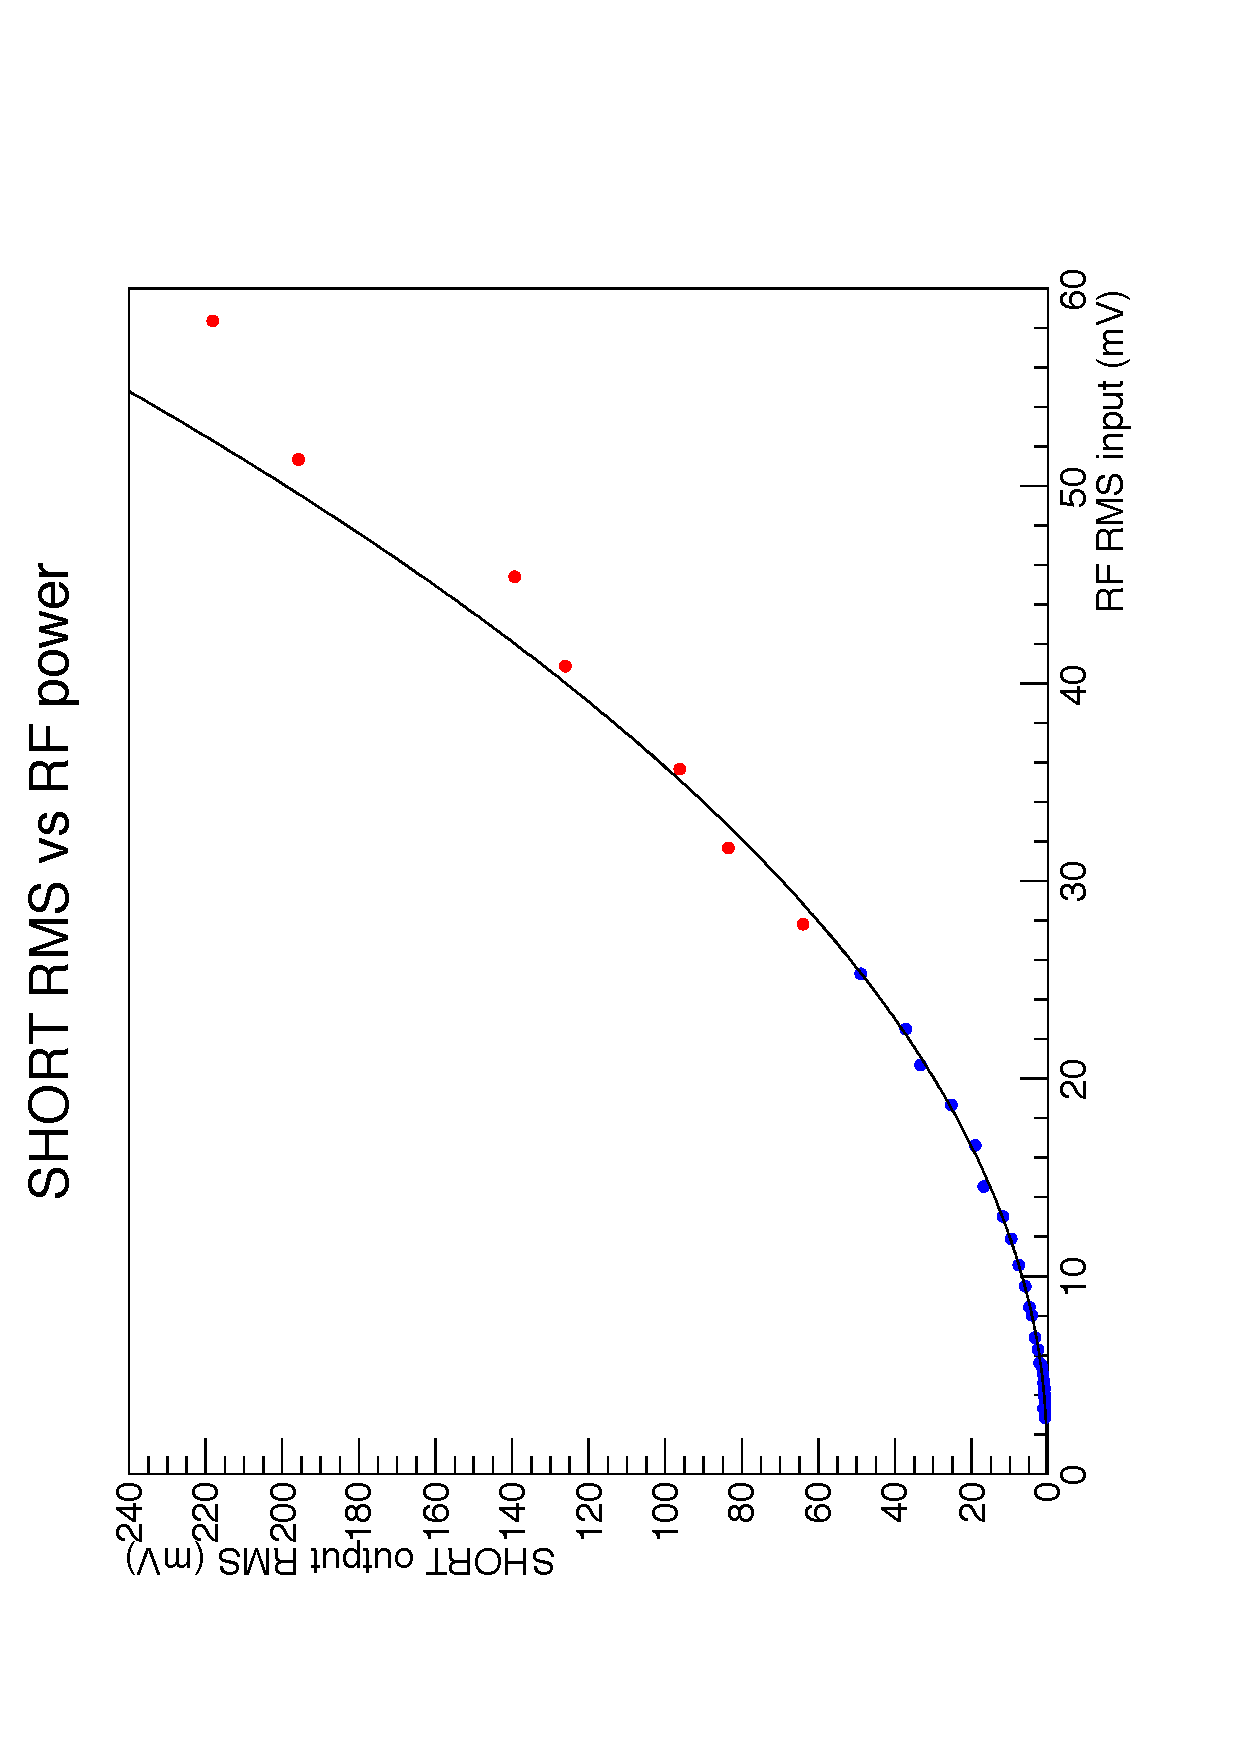
\includegraphics[width=0.9\textwidth]{figures/RMS_in_out}
	\caption{Measurements of the response of the SHORT tunnel diode "square law" RF power detector taken in Palestine TX in 2014.  Plot courtesy of Katie Mulrey.}
	\label{fig:SHORT_square}
\end{figure}
		
	
	\subsection{Trigger Hierarchy Overview}
		The triggering system is divided into several sub-triggers that layer hierarchically to arrive at a global trigger decision.   These range from the individual power law thresholding to a time windowed combinatoric trigger between multiple channels.  In ANITAIII, the trigger is split into a vertical (Vpol) and Horizontal (Hpol) trigger system, as the two differing particle shower sources (in ice neutrino interactions vs geomagnetically dominated air showers) will have mostly orthogonal observed polarizations.  These two trigger paths are identical and have equal weighting in the final global trigger decision.  
		
		The first L1 trigger level, is the comparator circuit on the FPGA between the output of the SHORT and a DAC. It is possible to adjust each channel individually to give an even weighting in the ultimate trigger decision.  This is accomplished by measuring the number of threshold crossing counts per time observed by each comparator circuit, called the pseudo-scalar rate, which is used as the input to a software Proportional Integral Derivative (PID) servo loop that controls the comparator voltage.
		
		The L2 trigger level is a phi sector specific time dependent windowing function that combines the L1 triggers from all three channels in a single phi sector.  A real plane wave signal incident on a phi sector will have a causal time separation between the physically separated antennas, while incidental noise threshold crossings will be uncorrelated in time.  To fire an L1 trigger, two causal signals are required to fall within this window.  The window is achieved by synchronously firing different length one shot pulses and logically combining them.  The bottom ring opens a 16ns window, the middle a 12ns window, while the top only opens a 4ns window. These timing offsets are used a a quickly determined metric for further discriminating on noise, and is limited primarily by the timing precision provided by the FPGA trigger electronics.  
		
		The final trigger, or L3 is a requirement that two neighboring phi sectors decide a L2 trigger within an 8ns window.  This leads to the ultimate requirement that four out of six like-polarized antenna channels with an overlapping field of view observe a transient power fluctuation.  There are two L3 triggers, one for each polarization, either of which firing issues a HOLD to a LAB3, beginning the digitization process.
		
		Additional information about the trigger is detailed below.  A diagram of the trigger hierarchy can be seen in Figure \ref{fig:trigPattern}.
		
\begin{figure}
	\centering
	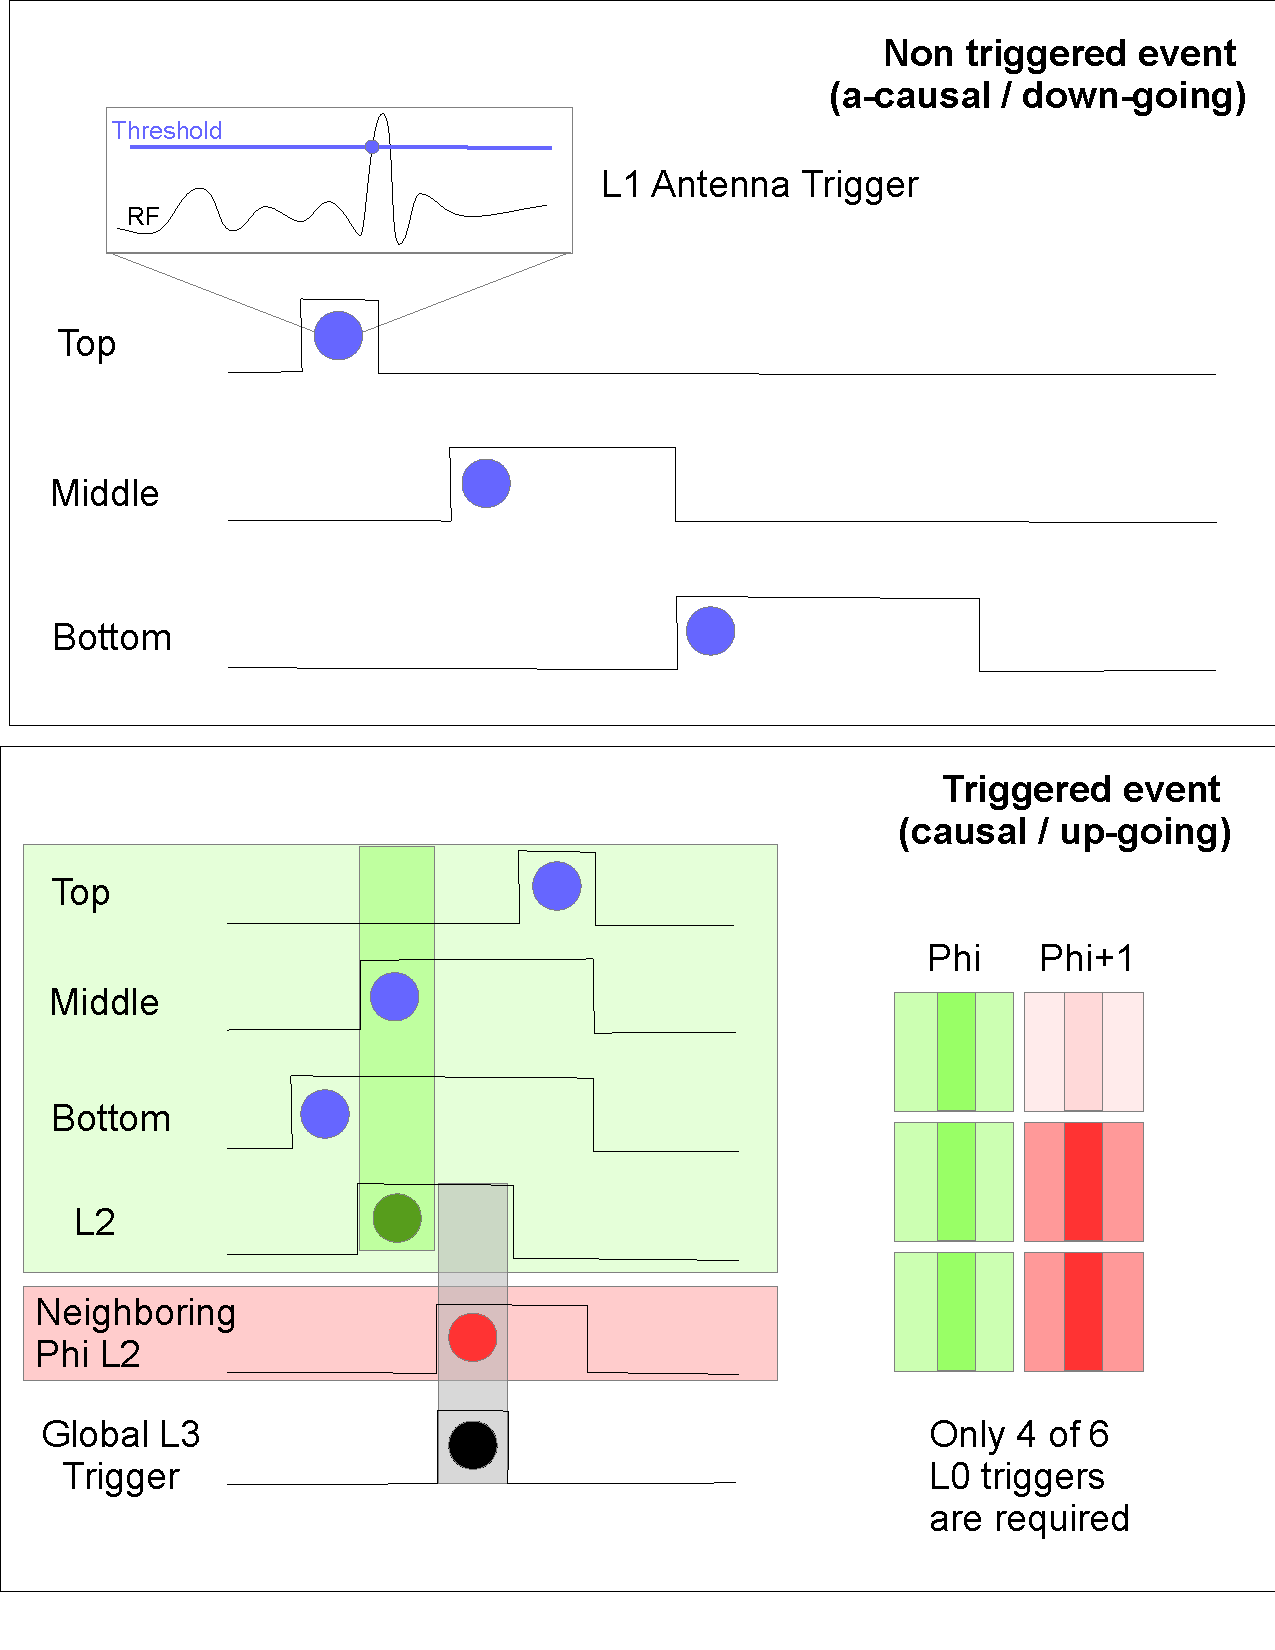
\includegraphics[height=0.8\textheight]{figures/triggerHeirarchy}
	\caption{A depiction of the trigger hierarchy for a non-triggered (top) and triggered (bottom) series of L0 triggers.  The blue dots denote an L0 trigger, and the green box represents the time of a L1  trigger.  Note the 4ns top ring window, the 12ns middle ring window, and the 16ns bottom ring window.  Two neighboring phi sectors with L2 triggers within a 8ns window cause a global L3 trigger (black).  Note also that, though not the case of depicted event, only two of the three rings are required to be in coincidence leading to a 4 out of 6 channel L1 trigger in two neighboring phi sectors}
	\label{fig:trigPattern}
\end{figure}


	\subsection{L1 Tiggering efficiency and quality}
		The trigger must make a trade off between efficiency and quality.  Efficiency is defined as the ratio of real signals selected for digitization over the total number of signals incident on the detector, and quality is the ratio of the number of true signal events over total selected events.  A perfect detector would have an efficiency of 1 and a quality of 1.  However in reality these values are both a function of the total maximum readout rate for the detector, which places a maximum limit on the number of events capable of being selected.  As an example, if the trigger constantly selected all moments in time it would be perfectly efficient, but the quality of the signal would be horrific.  Inversely, if the trigger was set to have perfect quality and only select extremely high power impulsive events, it would have poor efficiency for low Signal to Noise Ratio (SNR) signals.  The efficiency of the detector can be statistically measured by injecting signals of varying SNR at a known rate and observing the rate of measured signals.  The resulting characteristically shaped curve is shown in Figure \ref{fig:efficiency} of which the 50\% efficiency point. 3.5, is the defining metric.  This point will be directly related to the allowable accidental noise trigger rate, which was decided to be set at a rate where the payload would be "dead" for approximately 5\% of the time.
		
	\begin{figure}
	\centering
	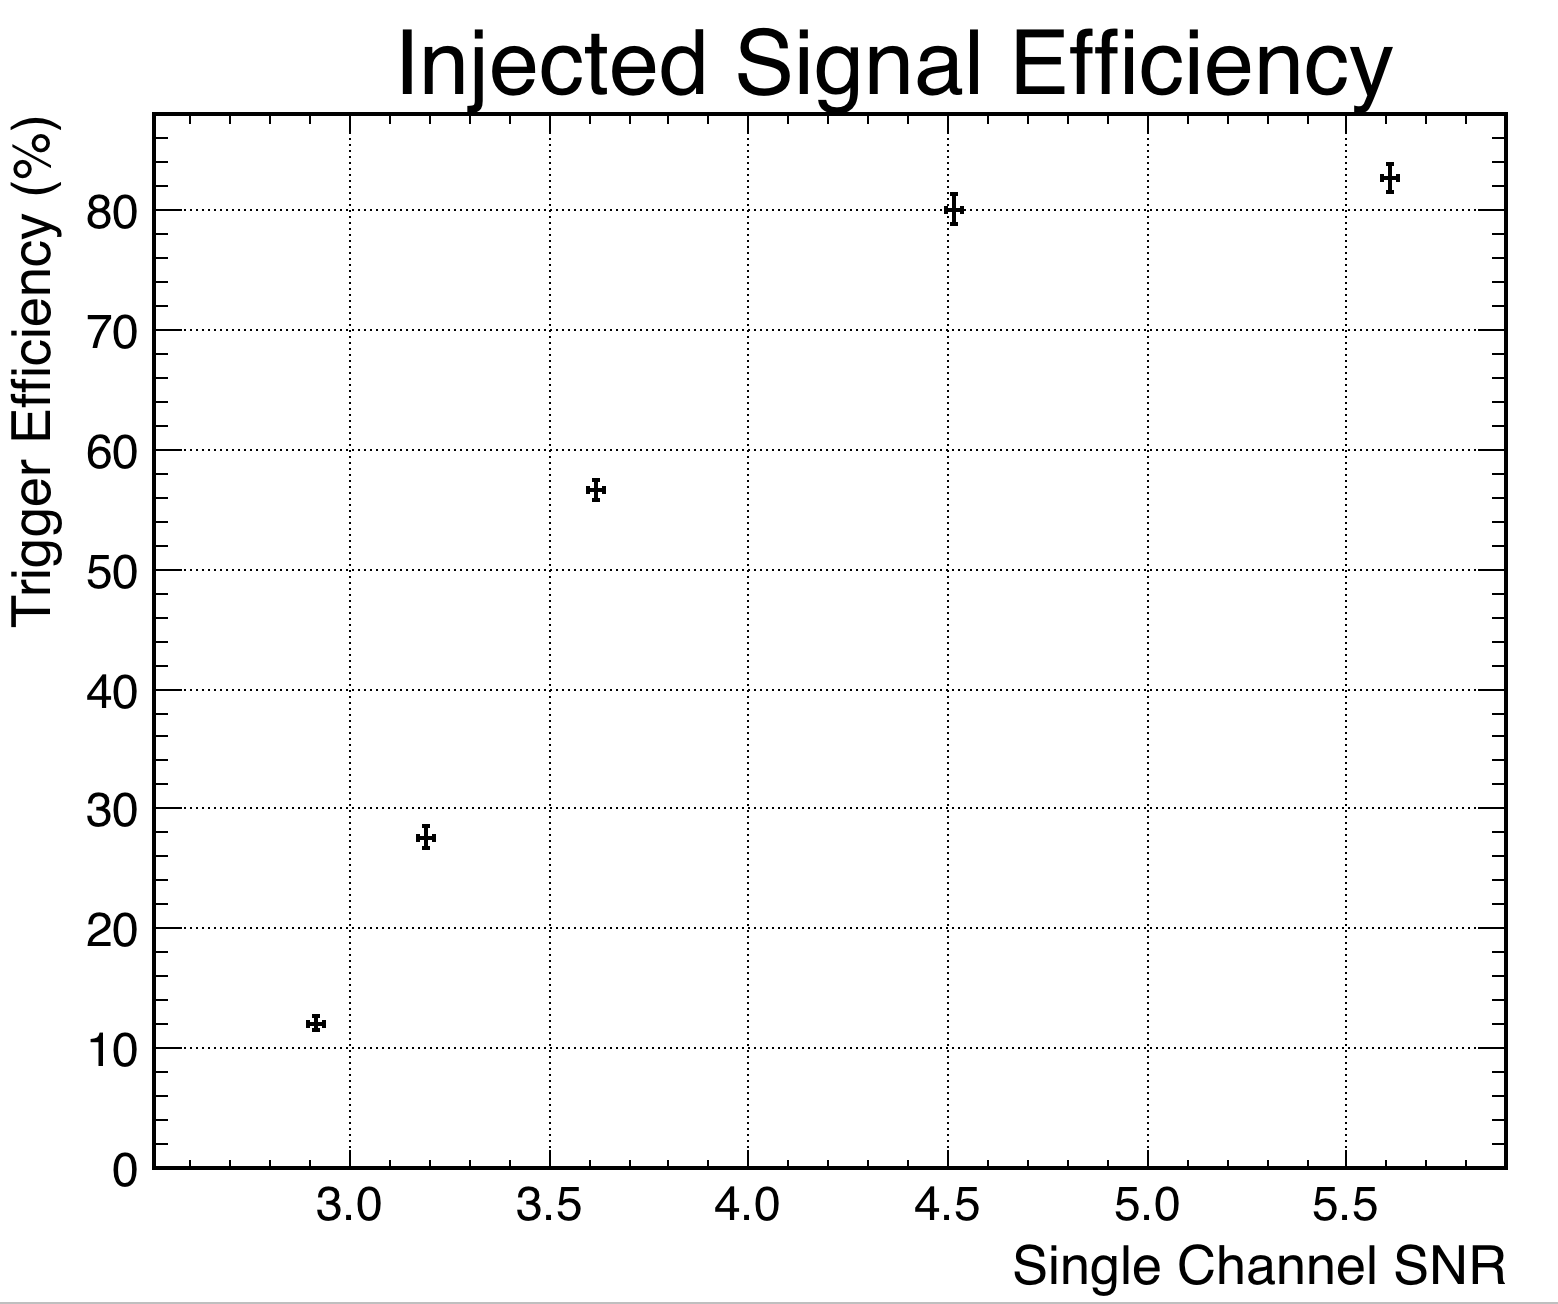
\includegraphics[width=\textwidth]{figures/palestineTrigEfficiency}
	\caption{The payload global trigger efficiency for injected impulsive signals, as measured in Palestine in the summer of 2014. Identical signals, each with the same SNR, were injected at a GPS stabilized 1Hz into all 6 channels in two phi sectors that share a polarization.  The signals pass through the entire signal chain and efficiency was calculated by averaging trigger rate.  The L1 PID rate goals for this measurement were 100kHz.  The 50\% efficiency point occurs at an SNR of roughly 3.5.  SNR is measured as averaged peak to peak signal voltage over noise RMS on a seventh signal propagated through an ANITA signal chain but measured on a laboratory oscilloscope.}
	\label{fig:efficiency}
	\end{figure}
		
		
	\subsection{L1 Optimization}
		What little room exists for optimizing the L1 trigger  lies in tuning the input power to the tunnel diode circuit.  The inverse-resistance region of the Esaki diode, where a decrease in voltage yields an increase in current flow, has a square law response which yields an output that is the square of the input.  This occurs at an extremely low power level, much below the minimum quantization level of the LAB3, and thus the power must be attenuated in the signal chain after the split between the trigger and digitizer paths.  If this attenuation is too great, changing the trigger threshold DAC setting a single bit for a specific channel would cause a large jump in the overall trigger rate of the system, and possibly allow a channel to dominate (or be excluded from) the global triggers.  However if the attenuation is too small, and the diode is pushed out of the inverse-resistance region, the response of the diode becomes linear, reducing its signal discrimination potential.
		
				
	\subsection{L2 Trigger Window Delay Limitations}
		As the physical offsets between the rings of antennas exceeds one 4ns FPGA clock period for most elevation angles of interest, it is possible to require a timing separation between the arrival of pulses between the separate antennas.  The expected delays between rings as a function of elevation angle, derived from photogrammetry, is shown in Figure \ref{fig:PhysicalDelays}.  This modification, made between the ANITAII and ANITAIII flights, decreases the incidental rate of the trigger, increasing the quality, while maintaining a low signal rate and high efficiency.  The requirement for an L2 trigger is that two windowing pulses overlaps (see Figure \ref{fig:trigPattern}).  This has the unfortunate side effect of allowing the bottom ring of antennas to unfairly bias the system. A noise L1 trigger generates a pulse with four times the time weight as one from the top ring, and is thus more likely to trigger the system.  
		
			
\begin{figure}
	\centering
	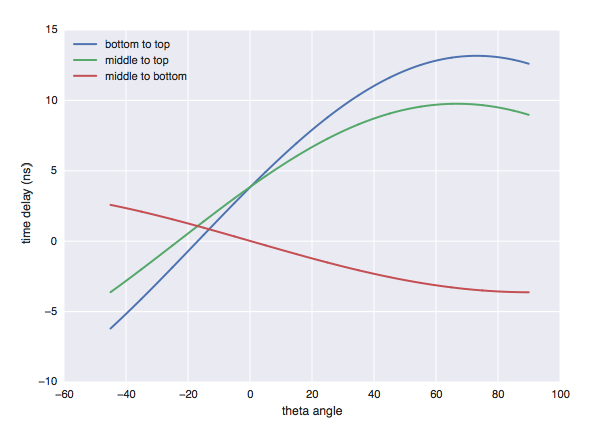
\includegraphics[width=\textwidth]{figures/PhysicalDelays}
	\caption{Propagation delays between antennas for an incident plane wave as a function of elevation angle.  Delays were derived using the antenna positions measured using photogrammetry.  These delays are used to determine the L2 trigger window locations.}
	\label{fig:PhysicalDelays}
\end{figure}	
		
	\subsection{Phi Sector Masking}
		In the ANITAI flight, it was discovered that noise sources on the continent and in the sky had the capability to dominate the trigger rate and effectively blind the entire payload despite a large fraction of the payload observing a thermal environment. To alleviate this issue, a system where an antenna or collection (phi sector) of antennas experiences a relative increase in trigger rate in comparison to the rest of the payload, those effected phi sectors will be excluded from participating in forming the global system trigger for a user adjustable time frame.  This allows the instrument to continue observing quiet areas of the continent and increasing the total livetime of the system.  There are additional nuances to this subsystem, including the possibility of very high power noise (or signal) events continuing to leak into the back and side lobes of the antennas from non-masked phi sectors, that need to be taken into account when making a measurement of the total instrumented area for a flight.  During the ANITAIII flight, several unexpected in-band satellite CW signals caused the phi masking to be heavily utilized, which is discussed further in the Cosmic Ray Search chapter.
		
%	\subsection{Differences between previous ANITA flight trigger systems}
%		In addition to changing the number of antennas, each ANITA flight has made modifications to the trigger subsystem in an attempt to increase the efficiency and purity of measured events.
		
%		The ANITAI instrument 
		
%		The ANITAII instrument separated each signal channel into 3 frequency sub-bands and one full banded trigger within the SHORT boards, before the tunnel diodes.  The reasoning for this was that neutrino signals are full band; a signal with power dominating a single band would be enough to disqualify an event from being a true signal event.  The requirement for a global trigger was several (how many?) bands, in addition to the full band.  It was decided after the flight that this did not did not decrease the quantity of triggers by a significant amount, and the banding scheme was removed in favor of accommodating additional channels (ANITAII did not trigger on Hpol and had 8 less antennas than ANITAIII, so 56 additional trigger channels were required).  This had the unwanted effect of allowing CW signals from northern satellites to overwhelm the detector during the ANITAIII flight.
		
	\subsection{Unbiased triggers}
		Any waveform readout caused by a global trigger has the systematic bias that it passed the trigger selection parameters.  To measure the thermal noise environment during the flight, two triggers that were uncorrelated to the trigger circuit were employed.  These were a software trigger (also know as the soft-trig) that was issued by the CPU at a frequency of 1Hz, as well as a GPS synced 1Hz trigger controlled by the Pulse-Per-Second (PPS) output of the G12 GPS unit.
		
		All events captured by the payload were marked with a trigType integer that described the source of their trigger decision.  The GPS and soft-trig signals can be easily selected in this way by excluding RF triggers.
		
		
\section{RF Power Monitor}
	An additional measurement of the RF signal is done by a broad band radio frequency power detector circuit.  The fast waveform data only provides 200ns of non-triggered, unbiased noise data per second (a 1Hz software trigger and a 1Hz GPS trigger), so a monitor that digitized a larger fractional percentage of time was desired.  This was accomplished on the SURF board using a commercial RF power monitor IC that converted the RMS voltage of the input signal into a log-magnitude proportional DC output that was digitized by an ADC and read out with the housekeeping diagnostic data.  This system, and the additional physics it provides, is discussed at length in Appendix A.

	
\section{GPS and orientation sensors}
	The payload is attached to a freely floating balloon with no control over rotational orientation or geographic location. This requires that the attitude be constantly monitored.  Multiple GPS systems, including two co-located ADU5 GPS heading receivers in conjunction with a single G12 GPS system, recorded the location of the payload throughout the flight.  The nine total GPS antennas, read out once per second, provide an absolute reference for the location and orientation of the payload with a resolution of a fraction of a degree.
	
	\subsection{Magnetometer}
		In addition to the heading information provided by the GPS systems, a magnetometer was attached to the payload and used to measure the vector components of the magnetic field throughout the flight.  This system, coupled with a model for the geomagnetic field, could be used as a functional compass, assuming an accurate position, that would corroborate the pointing information returned by the GPS systems.  As the GPS system remained functional throughout the flight, the major contribution from the magnetometer is as a validation of geomagnetic models in comparison to the GPS attitude measurement.
		
	\subsection{Sun Sensors}
		Many space borne experiments that require very high pointing and location precision are above the altitude where GPS begins losing accuracy and precision.  Their nominal orientation information is provided through the use of star sensors.  ANITA's flight path over Antarctica during the austral summer, when there is continual daylight, is able to use just one star to obtain accurate heading information.  With an accurate time and knowledge of the earth's rotation around the sun, one can use the four mounted angular sun sensors to determine the heading information for regions of time when the GPS is unavailable or unreliable.  As the sun is a single source, the full attitude of the payload can not be determined with this measurement alone. However for brief GPS outages, where payload location does not change dramatically, sun sensors can be used to reconstruct payload heading, which has a much faster time scale.  As the GPS system remained functional throughout the flight, the sun sensor data was not used.
		
\section{CPU, CPCI, and Data Readout}
	The custom LABRADOR digitizer ASICs and various control and command FPGAs are located on custom designed Printed Circuit Boards (PCBs) connected to a central processing unit (CPU) over a compact Peripheral Component Interconnect (cPCI) bus interface.  An image of the conductively cooled cPCI crate, in which all digitizing and readout electronics were housed, is visible in Figure \ref{fig:CPCIcrate}.  The Triggering Unit for Radio Frequency (TURF) board, which communicates with the SURFs to form the global trigger and propagate hold signals, is mounted to the back of this crate, connecting to the front mounted boards through cPCI Rear Transition Modules (RTMs).  Present within the cPCI crate is the CPU, a Line Of Sight (LOS) telemetry board, a digital and analog Acromag sensor readout board for reading various diagnostic subsystems, the 8 SURF boards,  and a TURF Input/Output (TURFIO) board, which provides access to the TURF from the front panel.
	
\begin{figure}
	\centering
	\includegraphics[width=\textwidth]{figures/cpciCrate_annotated}
	\caption{An annotated image of the cPCI crate prior to integration into the ANITAIII instrument box.  Labeled positions from left to right: the CPU, LOS board, Acromag boards, SURF boards, and TURFIO board.  Additional protective faceplates have yet to be installed in image.}
	\label{fig:CPCIcrate}
\end{figure}
	
	
\section{Data Storage and Telemetry}
	The most important piece of any experiment is the storage of the measurements for later analysis.  The rate at which data is taken during flight is designed to maximize the throughput of the electronics used to read out and store it.  It is not feasible to downlink the entirely of the stored information during flight due to limited bandwidth.  This necessitates the recovery of the payload, or at least the storage vaults, immediately preceding the flight.

	\subsection{Redundant data storage}
		The storage requirements for the flight were met by three separate digital storage form factors, each utilizing different methods.  This redundancy ensured that even in the event of a single failure the data from the flight would be preserved.  The first storage method was two identical Helium filled conventional spinning hard disk drives written to by the flight CPU over SATA.  The second method was a separately housed array of six Solid State Drives (SSDs), written to by a dedicated single board computer which received the flight data over an Ethernet link.  The third storage method, which ended being flown in an inactive state, was the RIFFRAFF handheld flash drive array; a complex system of microcontroller steered multiplexed commercial USB flash drives visible to the flight CPU.  During flight, a failure of the Ethernet link lead to the loss of the SSD array subsystem, leaving only the He Drive storage format intact.  Both drives survived the flight however, and two identical copies of data were recovered.
		In ANITA-III, the NTU device was a standalone CPU that connects with the flight CPU over ethernet and connected to six 1TB SSDs.  When one filled up, it would flip to the next.  It stopped communicating roughly a third of the way into the flight (probably because the ethernet power cable wiggled loose and all ethernet connectivity ceased), and was not needed due to the success of the He drive system.
		
	
	\subsection{Telemetry}
		Downlink of data taken during flight and uplink of commands to change flight configuration are transmitted to and from ground receivers over several systems.  In order of decreasing data trasmission speed, they are the Line Of Sight (LOS) transmitter, an Iridium Pilot$_{\text{\textregistered}}$ Openport UDP link, a NASA Tracking and Data Relay Satellite System (TDRSS), and an Iridium$_{\text{\textregistered}}$ low rate downlink.  These systems allow in-flight diagnostics of the ANITAIII instrument, as well as an ability to make pre-defined alterations to instrument control configurations, depending on need.  Shortly after flight, the Iridium Pilot$_{\text{\textregistered}}$ Openport link failed for unknown reasons.  However, the remaining systems were successful in allowing flight operators to debug and fix several issues that cropped up during the flight.  %The specified downlink rates for each of these systems can be seen in Table \ref{tab:telemRates}.
		
	\begin{table}
	
	\end{table}
		
	\subsection{GPU prioritization}
		The data limitations of the various telemetry downlink systems allow only a fraction of the total data rate to be transmitted.  This limitation motivates a prioritization system in order to only send down events that pass a limited set of post-digitization analysis cuts.  This would allow a limited set of analyzable signals in the event of a catastrophic system failure or non-recovery of the payload.  The two major figures of merit for discriminating between incidental thermal noise events and impulsive signal-like events is the normalized peak height of an interferometric pointing map, and the peak of the Hilbert envelope of the coherently summed waveform for the respective map peak incidence angle.  These time-consuming, computationally intensive, physical baseline dependent, multiple channel correlation processes are nominally done offline in the analysis phase of the experiment, and is likewise further discussed in the analysis chapter of this thesis.  However, to accomplish the task in real time, as events are being logged by the instrument, a Graphical Processing Unit (GPU) linked with the flight CPU, was utilized to parallelize the computations and reduce any specific event readout's required processing time to that of the minimum instrument readout time.  These values were then used to determine a priority for each event and assigned a priority for telemetering.  The main work on this system was done by Ben Strutt of University College London, and details on its operation and results can be found in his doctoral thesis \cite{BenSThesis}.  Since the instrument was recovered, these computations are re-done for this thesis, and the priority value was not used.
		
\section{Balloon and Flight}
		The ANITA instrument is suspended from a NASA zero pressure, long duration high altitude balloon over the continent of Antarctica.  The partially inflated balloon and launch team immediately before launch of the ANITAIII payload can be seen in Figure \ref{fig:Launch}.  The 34 million cubic liter balloon, when filled with Helium gas, has a nominal float altitude of 130kft (40km) and has been rated to survive for up to 60 days.  As the balloon ascends, it expands as the gas equilibrates to the surrounding atmosphere, which decreases in density with altitude. The balloon can be seen, partially expanded, in Figure \ref{fig:Balloon}.  The balloon floats freely after launch, with no aeronautical controls with the exception of a ballast hopper which can be dumped as Helium escapes from the balloon. The circumpolar winds present in Antarctica provide a circular trajectory around the continent.  The requirement of a balloon recovery for a complete physics dataset necessitates terminating the flight when the balloon heads northwards towards the ocean.  
		
		The ANITAIII flight launched on December 17th 2014 at 19:23 UTC and flew for 22 days before being terminated near Australia's Davis station as it moved close to the coast.  The flight path of the payload is shown in Figure \ref{fig:A3FlightPath}.

\begin{figure}
\centering
	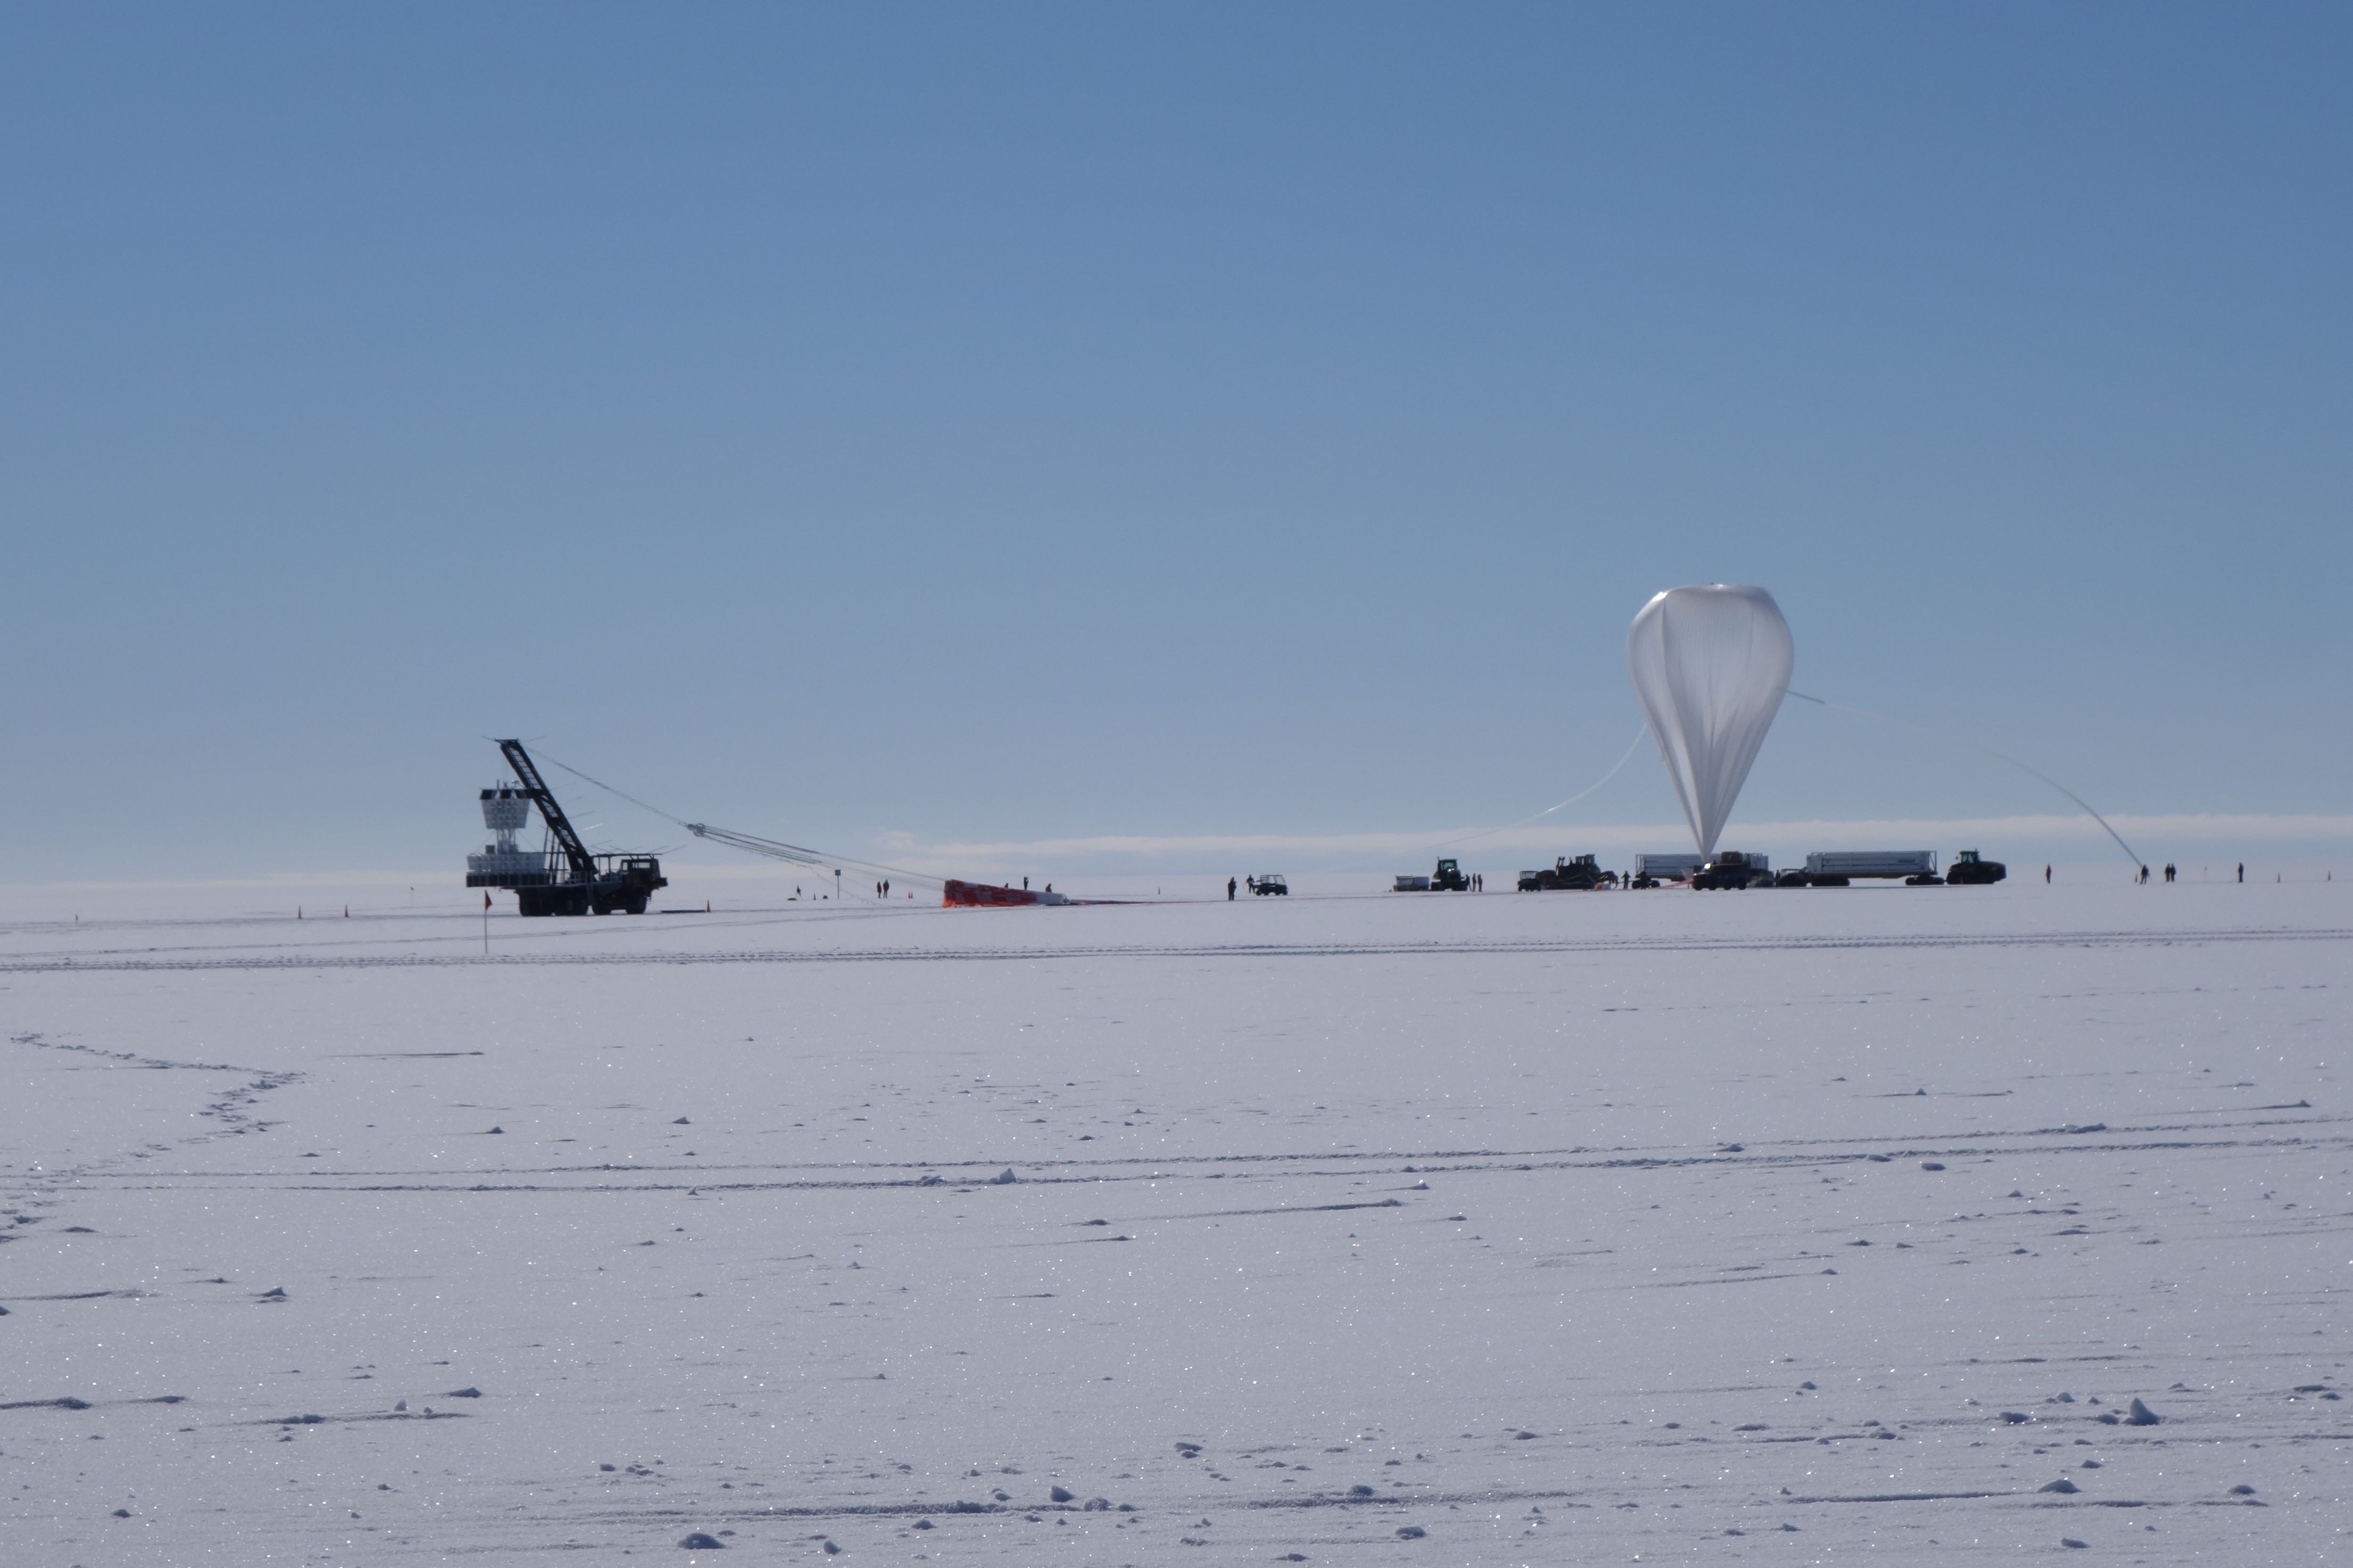
\includegraphics[width=\textwidth]{figures/Launch}
	\caption{Image of the launch vehicles, the balloon, and the ANITAIII instrument immediately proceeding launch on December 17th, 2013.  On the left of the image is the LDB launch vehicle, named The BOSS, suspending ANITA.  Attached to ANITA and the launch vehicle laying across the ice is the termination package, including a parachute for decent, and balloon.  The tanks in the background are transportation canisters for the Helium gas, which is filling the balloon through the transparent hoses attached on the sides.}
	\label{fig:Launch}
\end{figure}
			
		
\begin{figure}
\centering
	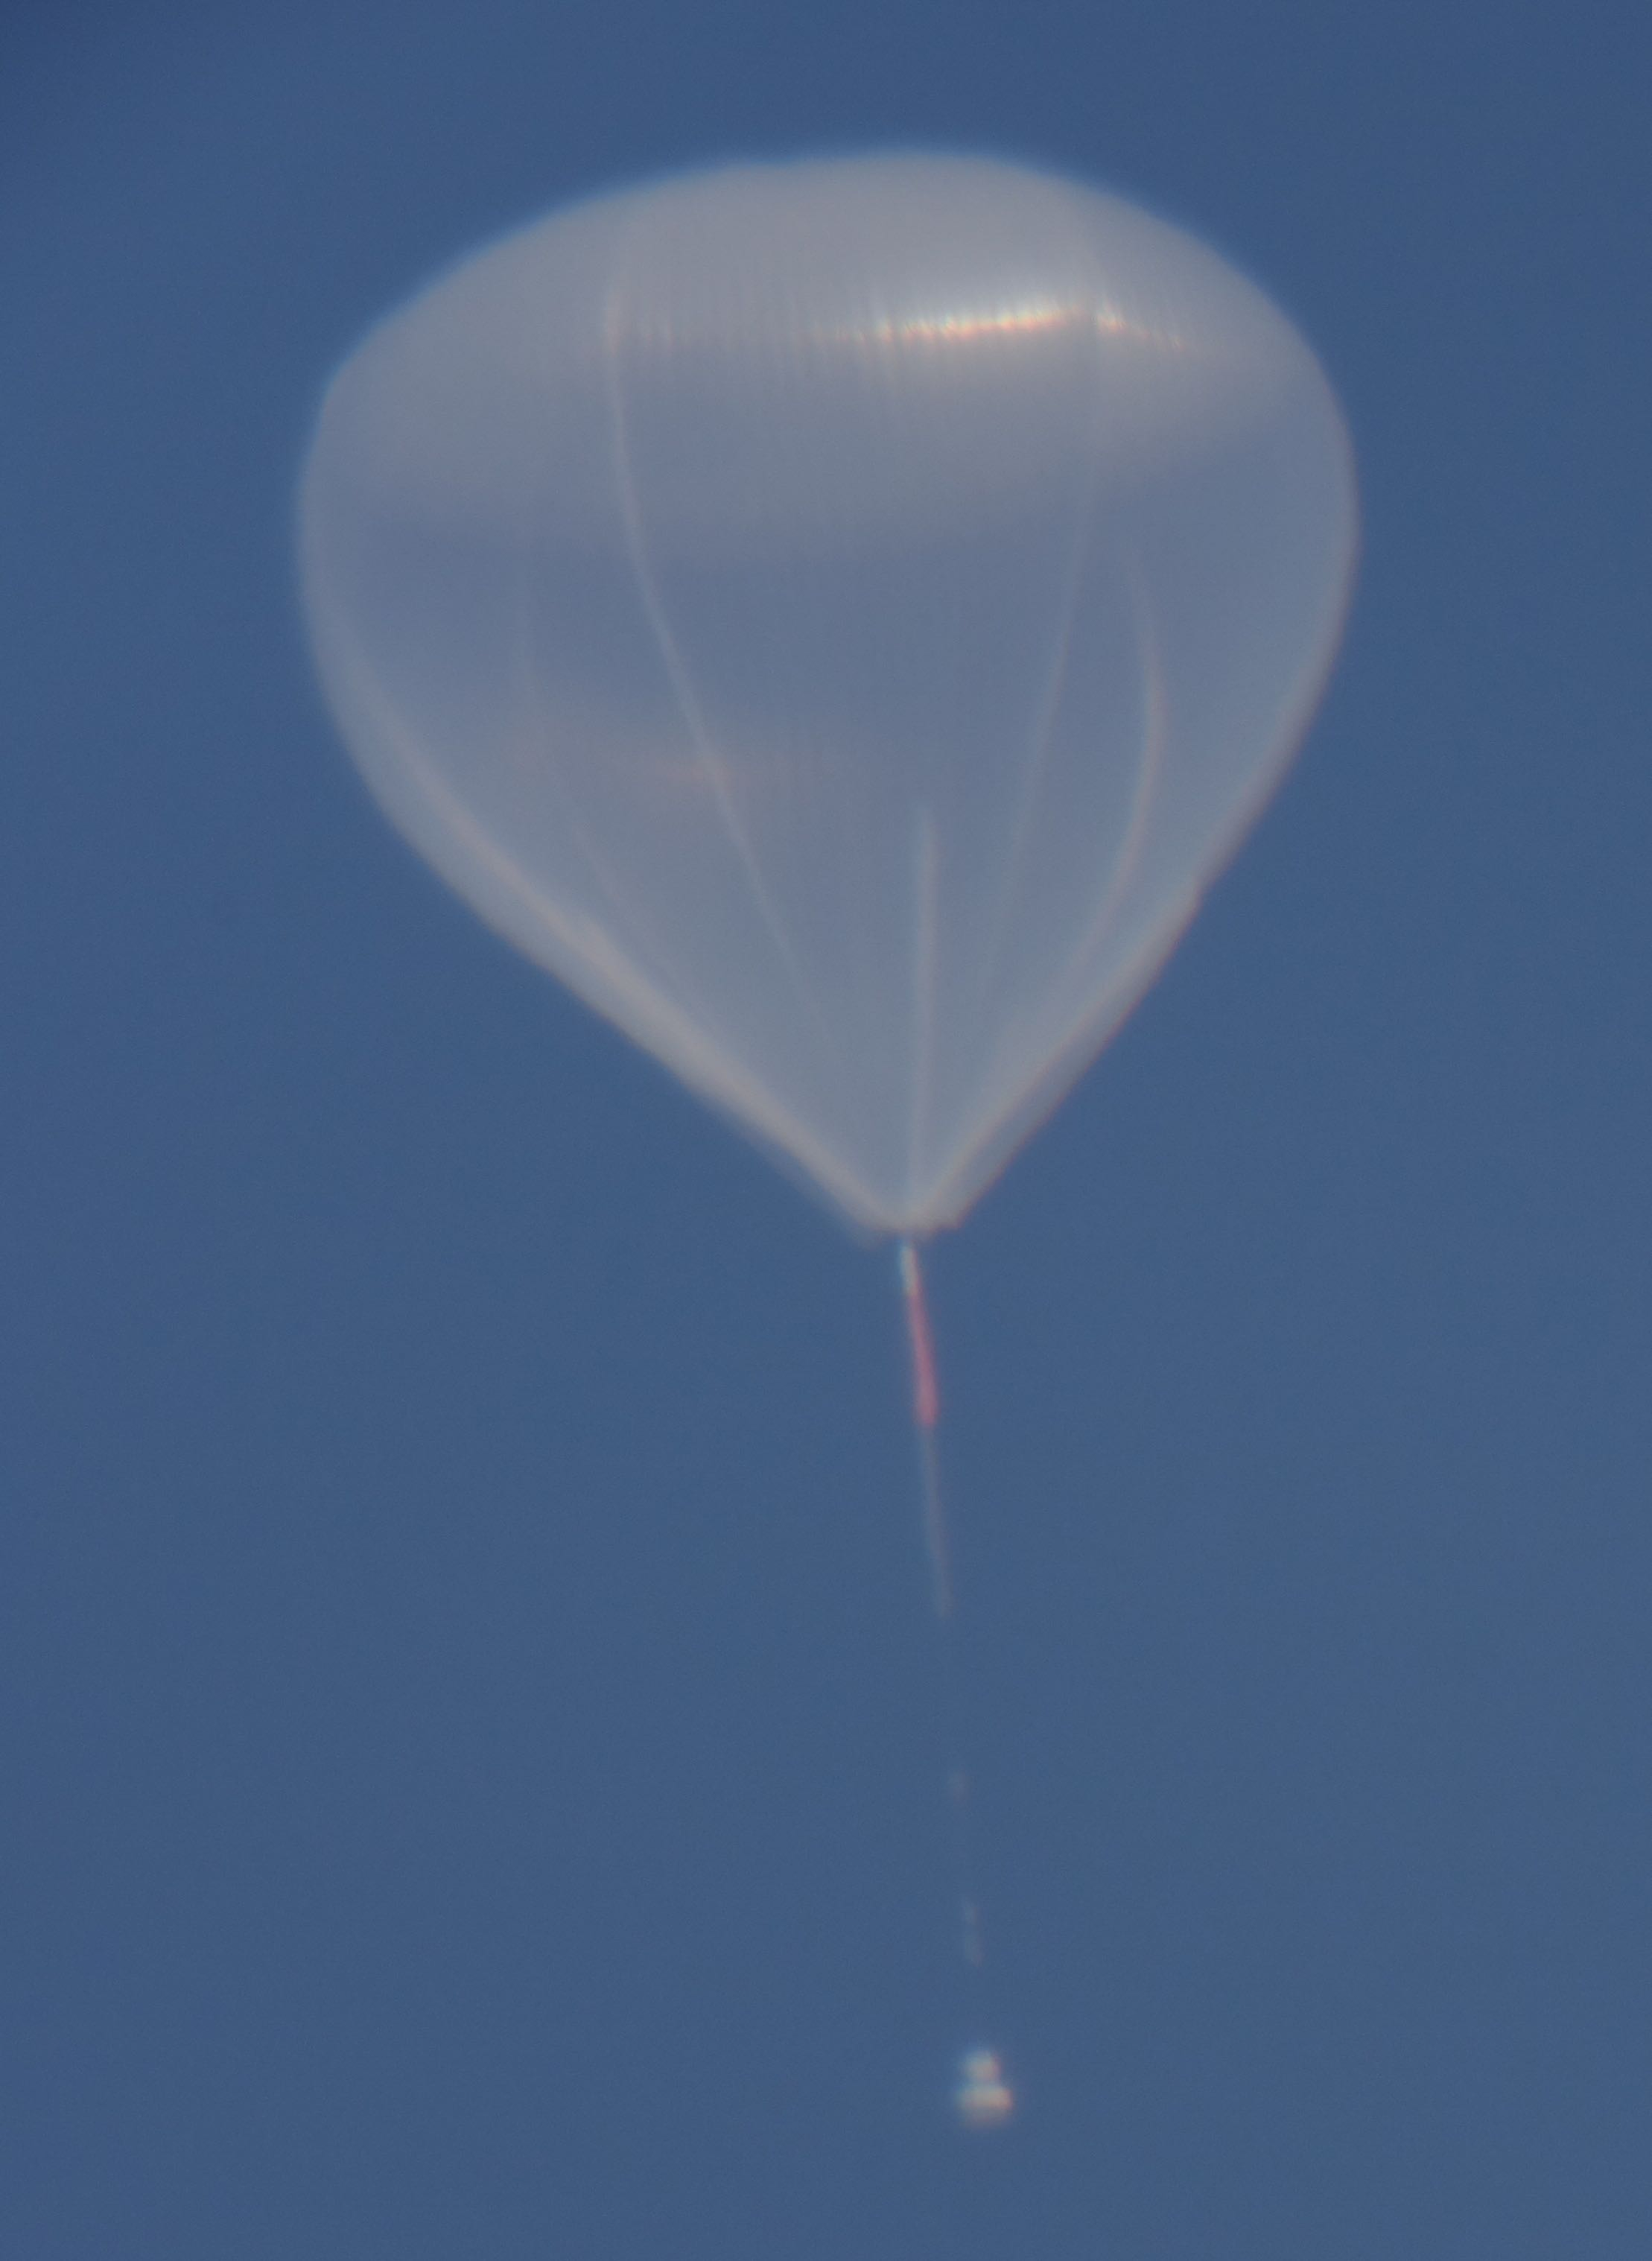
\includegraphics[height=0.9\textheight]{figures/CelestronBalloon}
	\caption{Image of the ANITAIII payload approximately 5 hours after launch. Image was captured with aid of a Celestron telescope and captured from the LDB facility. }
	\label{fig:Balloon}
\end{figure}

\begin{figure}
\centering
	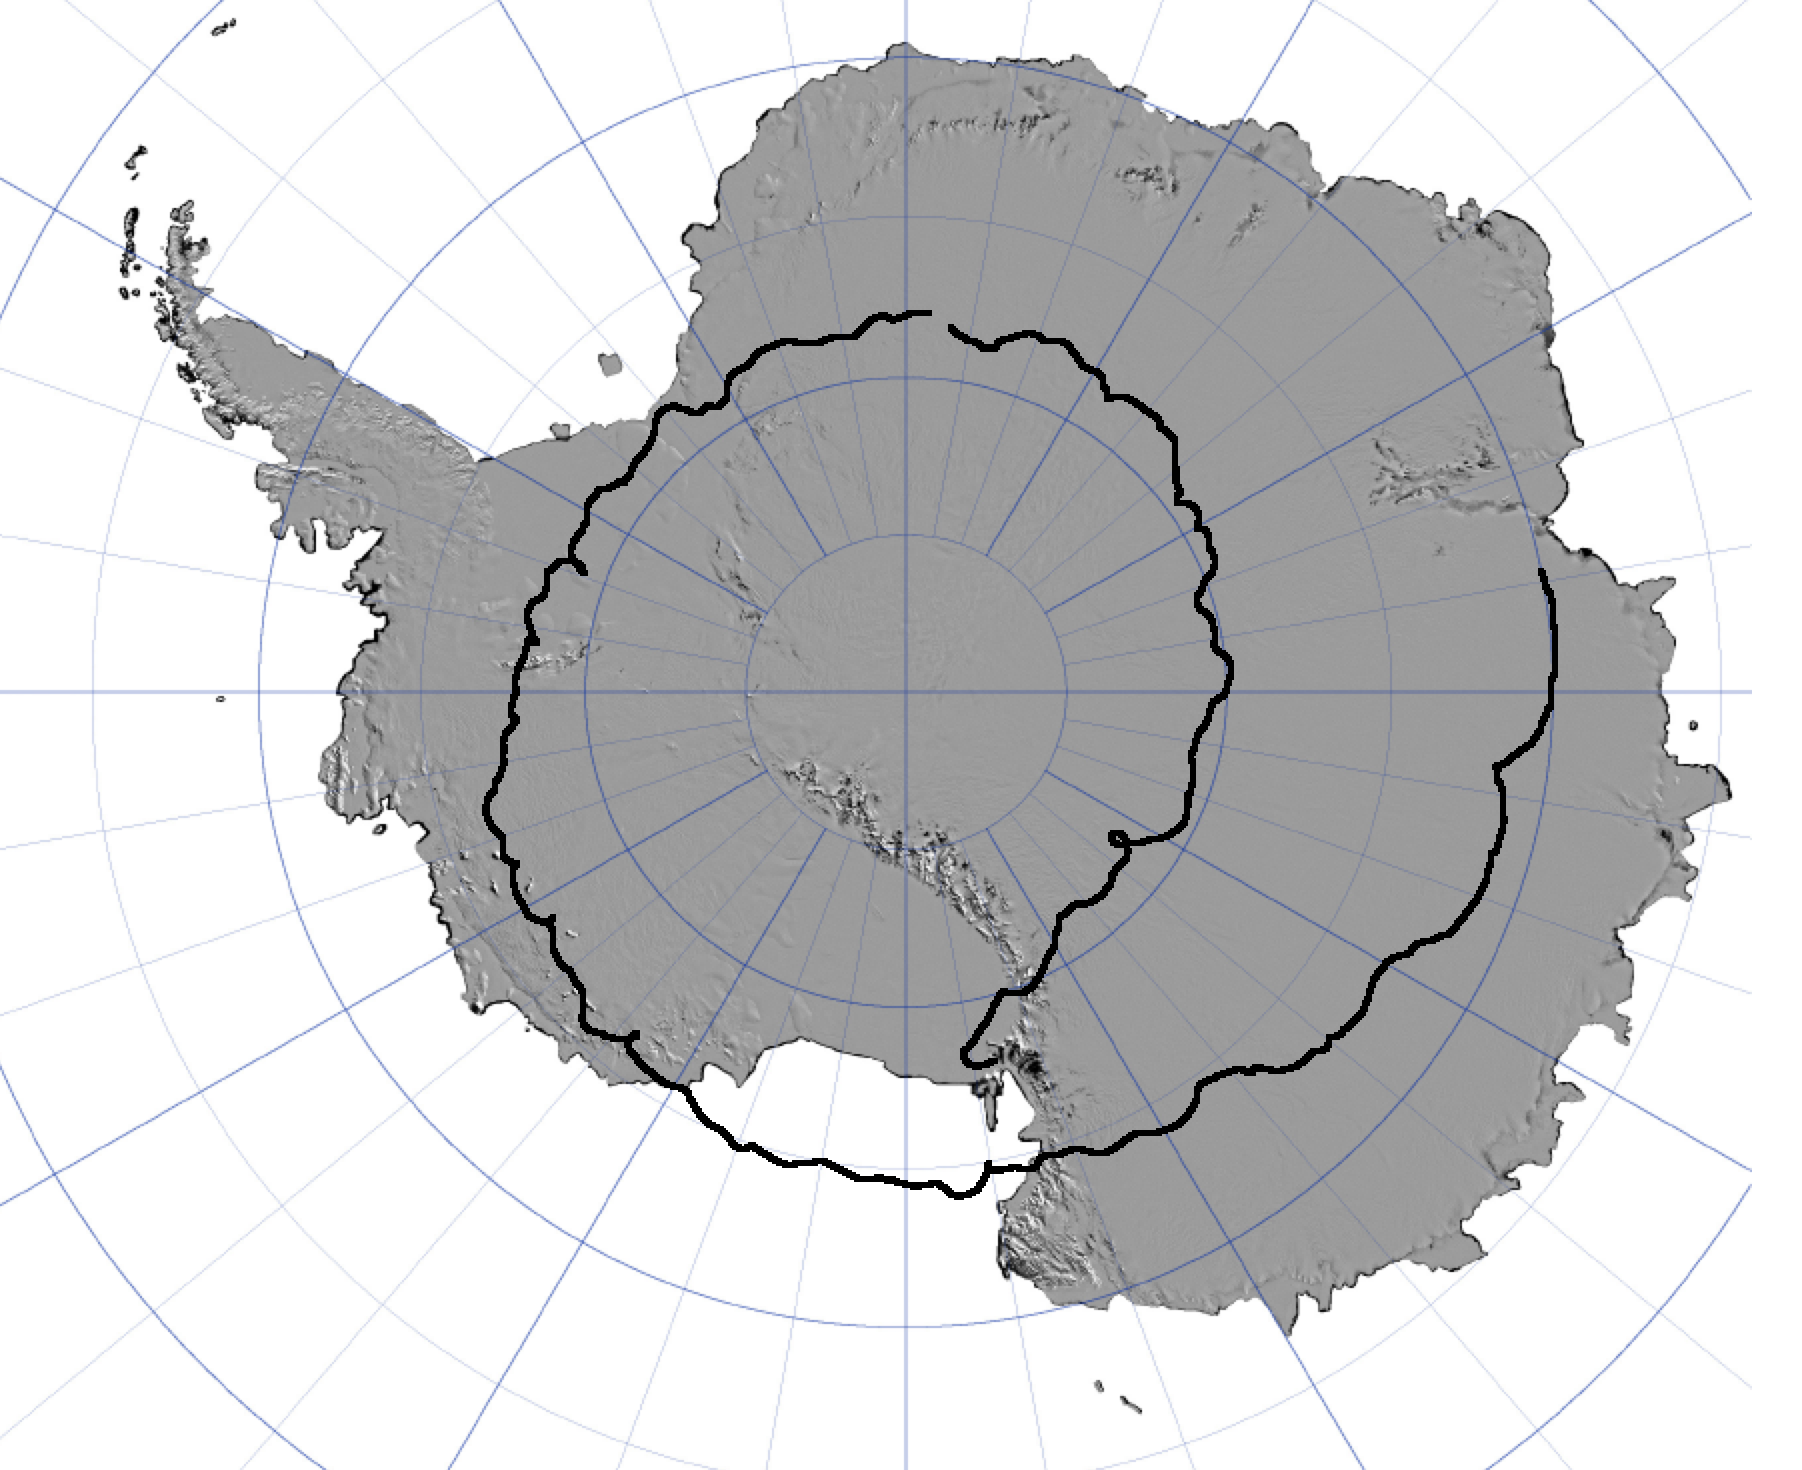
\includegraphics[width=\textwidth]{figures/A3FlightPath}
	\caption{Flight path of the ANITAIII instrument as recorded by the onboard GPS.  The gap at the ``top'' of the arc (grid north) corresponds to a 11 hour downtime experienced by the payload (discussed in the Analysis chapter)}
	\label{fig:A3FlightPath}
\end{figure}


		

%	\subsection{In Flight Modifications}
%		The majority of the ANITA3 flight required very little input from ground operators.  However there were some minor issues in the beginning of the flight that required fixing, and one in the middle of the flight that resulted in lost data.
		
%		At the beginning of the flight, the default time persistance values for phi masking were set too high, resulting in the entire payload becoming masked as it rotated.  The solution to this was to lower user configurable time persistance values via ground operator commands pre-programmed into the payload.  This was tuned so that phi masking would be correctly cycled off as scalar rates dropped back to manageable levels.
		
